\documentclass[12pt]{article}

\usepackage{pdflscape}
\usepackage[left=2.5cm, right=2.5cm, top=2cm, bottom=3cm]{geometry}
\usepackage{mathtools}
\usepackage{amssymb}
\usepackage{tikz} \usetikzlibrary{calc, arrows.meta, intersections, patterns, positioning, shapes.misc, fadings, through,decorations.pathreplacing}
\usepackage{amsthm}
\usepackage{subfig}
\usepackage[sc]{mathpazo}
\usepackage{ragged2e}
\usepackage{setspace}
\usepackage{xcolor}
\usepackage{tikz}
\usepackage{tcolorbox}
\usepackage[dvipsnames]{xcolor}
\usepackage[colorlinks=true, allcolors=blue, pdfstartview=FitH, pdfpagelayout=OneColumn]{hyperref}
\usepackage{calc}
\usepackage{tabularx}
\usepackage{multirow,bigdelim}
\usepackage{enumitem}
\usepackage[margin=10pt,font=small,labelfont=bf,labelsep=space,format=plain]{caption}
\usepackage[authoryear, longnamesfirst]{natbib}
\usepackage{datetime}
\usepackage{float}
\usepackage{graphicx}
%\usepackage{pgfplots}
\usepackage{tikz}
\usepackage{titlesec} % Add this line
\usetikzlibrary{positioning,shapes}
\usepackage{threeparttable}
\newdateformat{monthyear}{\monthname[\THEMONTH] \THEYEAR}
%\setlength{\parindent}{0cm}
\usepackage{booktabs}
\theoremstyle{plain}
\newtheorem{theorem}{Theorem}
\theoremstyle{plain}
\newtheorem{proposition}{Proposition}
\theoremstyle{plain}
\newtheorem{assumption}{Assumption}
\theoremstyle{definition}
\newtheorem{definition}{Definition}
\theoremstyle{plain}
\newtheorem{corollary}{Corollary}
\theoremstyle{definition}
\newtheorem{condition}{Condition}
\theoremstyle{plain}
\newtheorem{lemma}{Lemma}
\theoremstyle{remark}
\newtheorem{remark}{Remark}
\theoremstyle{definition}
\newtheorem{example}{Example}
\theoremstyle{definition}
\newtheorem{result}{Result}
\theoremstyle{plain}
\newtheorem{observation}{Observation}
\newcommand{\ubar}[1]{\text{\b{$#1$}}}
\DeclareMathOperator*{\argmax}{argmax}
\DeclareMathOperator*{\diff}{d}
\def\citeapos#1{\citeauthor{#1}'s (\citeyear{#1})}
\onehalfspacing
\usepackage{graphicx} % Required for inserting images
\usepackage{todonotes}

\usepackage{lmodern} % Add this line

\title{\normalfont \LARGE Another Brick in the Wall? The Educational Effects of Repurposed Mafia Properties} 
\vspace{0.5cm}
\author{Victoria Biagi\thanks{University of Liverpool, Liverpool L69 7ZH, United Kingdom; \texttt{Victoria.Biagi@liverpool.ac.uk}. I would like to thank Giuseppe De Feo, Jakub Lonsky, and Balazs Murakozy for their guidance in the project. I thank Michaela Sviatschi and Noemi Mantovan for their important suggestions. This paper has also benefited from the suggestions from Sonia Balhotra, Jacopo Bregolin, Ian Burn, Enrico Cavallotti, Anand Chopra, Gianmarco Daniele, Giacomo De Luca, Ruben Durante, Rema Hanna, Abhinav Khemka, Gema Lax-Martinez, Giovanna Marcolongo, Olivier Marie, Bruno Martorano, Giovanni Mastrobuoni, Christian Morabito, Paolo Pinotti, Zachary Porreca, and several presenters met at the Women in State Capacity Conference (Oxford, 2025), NWSSDTP Doctoral Conference (Lancaster 2024), and the 9th Workshop on the Economics of Organised Crime (Edinburgh, 2025). Special thanks go to the confiscated assets director from the association Libera Tatiana Giannone and the NGO Centro Studi Pio la Torre which gave me great knowledge about the practices of reuse of Mafia properties, the context of Mafia strongholds, and allowed me access to their survey data. I thank the Italian Ministry of Education which helped me through the collection of my data as well. All the mistakes are mine.}}
\normalsize
\date{September 2026}

\begin{document}      
\maketitle
\justifying

%%%%%%%%%%%%%%%%%%%%% ABSTRACT %%%%%%%%%%%%%%%%%%%%%%%%
 \begin{center}
    \textbf{\large{Abstract}} \\ 
 \end{center}
 Italy's anti-Mafia legislation allows confiscated Mafia properties to be converted into educational, cultural, and welfare facilities where local NGOs offer various social activities specifically targeting the youth and other vulnerable groups. This study provides the first causal evidence on how exposure to these repurposed spaces affects students' dropout rates by changing their attitudes toward educational and criminal pathways. Using school-level geo-referenced data from 2015 to 2022 and exploiting the staggered timing of property repurpose, I investigate changes in local dropout rates. Results find a significant reduction in dropout rates of approximately 36\% for students living near repurposed properties. I show that this policy reshapes students' beliefs, reducing the appeal of Mafia networks while increasing the value of formal education. The effects are not explained by gentrification, additional educational support, or civic engagement levels.  \par


%%%% KEYWORDS %%%
\textbf{Keywords:} Mafia; property; Italy; education;  NGOs; perception; State. \\
\textbf{JEL Codes:} R23, H72, I25, K42.  \\
\textbf{Conflict of interest:} None.
% Start writing your thesis here:
\newpage
\titleformat{\section}{\normalfont\Large\bfseries}{\thesection}{1em}{}
\titleformat{\subsection}{\normalfont\large\bfseries}{\thesubsection}{1em}{}
\titleformat{\subsubsection}{\normalfont\normalsize\bfseries}{\thesubsubsection}{1em}{}


\FloatBarrier
\section{Introduction}
\label{sec:jmp_intro}
%\normalfont \section{ Introduction}


The detrimental effects of organised crime on education are well-documented, particularly in areas controlled by Mafia-type groups where these effects are highly localised. Juveniles can be directly recruited by Mafia affiliates, but they can also be affected by criminal social norms and behavioural codes \citep{van_dijk_children_2019, kleemans_criminal_2008}. In Italy, Mafia groups have been shown to systematically distort youth's aspirations about investing in education versus pursuing criminal alternatives \citep{acemoglu_weak_2020,coniglio_organized_2010, caglayan_organized_2017}, prompting policymakers to develop targeted interventions for Mafia-affected communities. Among these interventions, the most significant is the Mafia Confiscated and Reallocated Assets Reuse Policy (CRR) implemented nationwide since 1996. Under this policy, the confiscated Mafia properties, former symbols of territorial control and criminal activity, are converted into educational, cultural and welfare facilities, where local NGOs offer various social activities specifically targeting young people and other vulnerable groups. These repurposed spaces aim to transform former Mafia strongholds into community assets that foster legitimate social bonds and provide alternative role models \citep{falcone_beneitalia_2016}. The question remains, however, whether this symbolic transformation translates into measurable social and economic benefits for the youth. Existing case studies document positive effects on communities' social participation \citep{nazzaro_il_2021, martone_politiche_2020}, while establishing that Mafia social bonds may prove resilient to these policy efforts. I address this empirical gap by documenting the evolution of repurposing practices and their subsequent impacts on educational outcomes. \par
\medskip
In this paper, I construct a novel dataset and leverage the quasi-experimental variation in the timing and use of repurposed Mafia properties to provide the first empirical evidence on their impact on local education. Moreover, I investigate the mechanisms driving these effects by examining several potential channels. I focus on the ten main urban centres in historically Mafia-ridden regions, which concentrate the majority of confiscated Mafia properties\footnote{The cities I investigate include Naples, Salerno, Bari, Taranto, Foggia, Reggio di Calabria, Palermo, Messina, Catania, and Siracusa. Focusing on the major Mafia-ridden urban centres allows me to leverage the necessary variation in Mafia real estate reallocation and repurposing practices.}. Young people's educational outcomes tend to be especially low in these regions, with dropout rates reaching concerning levels: 14.6\% in Campania and Apulia, and 18.8\% in Sicily against a national average of 12.7\% \citep{save_the_children_alla_2022}. Local NGOs and municipalities manage these repurposed properties to operate programs focused on education, culture, skills training, and social services, with 45\% of them explicitly targeting the youth. In this setting I exploit the staggered repurpose of Mafia properties, conditioning on neighbourhood and municipality-level attributes. \par
\medskip
I construct a novel database combining information scraped from the website \emph{\href{https://www.confiscatibene.it/}{Confiscatibene}}, internal surveys from the anti-Mafia Association \emph{Libera}, municipal records, and administrative data on the precise locations of confiscated properties. I digitised Antimafia Investigative Directory maps measuring the baseline Mafia presence, and I draw on Ministry of Education records covering high school enrolment, graduation rates, and student ages. I further collect NGO location data from the Ministry of Labour, survey data about the students' perception of the Mafia, and the 2011 census data to account for baseline socio-economic characteristics. \\
To estimate the effect of this policy on educational outcomes, I employ a DiD design that compares educational outcomes in areas where Mafia properties have been repurposed to those located in unaffected areas over the same period. My main outcome variable tracks dropout rates by following the same student cohorts across high school grades. This allows me to focus on students older than 16, which corresponds to the end of compulsory schooling age in Italy. This exercise allows me to measure students' dropout decisions when continued schooling becomes voluntary. Given the absence of official high school districts in Italy, I construct school catchment areas based on the distance between high schools and census blocks\footnote{Census blocks are defined by the Italian Institute of Statistics and typically contain on average 200-400 inhabitants.}, defining them as treated if they contain at least one repurposed Mafia property and as control otherwise. In this setting, I estimate the average treatment effect on the treated (ATT) with traditional TWFE models as well as modern DiD estimators following \citet{sun_estimating_2021}. \par
\medskip
The effective repurpose of former Mafia properties significantly reduces dropout rates by approximately 36\% relative to the mean among students who have reached the age when formal education is no longer compulsory. This effect is  consistent with previous research on the effect of the Mafia on education. \citet{caglayan_hindering_2021} find that Mafia presence reduces graduation rates by 25\% in Northern Italy.  Additionally, I test the intensive margin of the treatment, finding that the results are particularly strong where more than 1 property has been repurposed in the area. I use the count of reused properties rather than the binary treatment indicator and I employ the \citet{de_chaisemartin_difference--differences_2024} estimator to account for dynamic treatment effects; I find that each additional confiscated property repurposed is associated to a 12\% decrease relative to the mean\footnote{Given that treated municipalities have an average of 2.22 confiscated assets, these estimates are remarkably consistent $(12\% \times 2.22 \approx 27\%)$, providing strong evidence for a linear dose-response relationship where the intensity of reused activities matters proportionally for the magnitude of effects.}. The consistency across binary and continuous treatment specifications reinforces confidence in the validity of the main results.  \\
Moreover, the heterogeneity analysis reveals several important patterns. First, the effects I estimate are particularly strong in schools underperforming across multiple domains at the baseline, including students’ performance in national standardised assessments, citizenship competences, the quality of the learning environment, and the local engagement with families and local community. This suggests that repurposing interventions are most effective in contexts characterised by institutional weaknesses, where the visible reclaiming of a formerly Mafia-owned property might send a particularly strong signal of the State's presence and the community's capacity to reclaim its own space.
Second, technical high schools emerge as the primary beneficiaries of the repurposing interventions, exhibiting sustained reductions in dropout rates that become statistically significant between years 2 and 4 post-treatment and persist throughout the observation period. This contrasts sharply with academic and vocational high schools, which display mixed and statistically insignificant effects. This heterogeneous pattern aligns with the distinct institutional contexts and student populations served by each educational track. Technical schools serve students who often come from backgrounds that value practical skills alongside academic preparation, making them particularly sensitive to localised improvements that enhance educational engagement. Unlike vocational students, who can enter the workforce when they turn 16 with a professional certificate, technical high school students are expected to complete the full five-year program, exposing them to a longer period of risk during which dropout becomes increasingly likely. Last, the estimated effects are entirely driven by the repurpose of \emph{operational Mafia properties}, namely villas and apartments that symbolised the local control of the Mafia family. Across activity types, the point estimates are of broadly similar magnitude; the effect reaches significance only for cultural activities, so the distinction reflects greater precision rather than a categorically larger effect. This is consistent with the interpretation that what drives the reduction is less the specific activity offered than the signal the reclaimed space itself sends. 
Together, these heterogeneous effects point to a common mechanism:by signalling the retreat of criminal influence and the return of legitimate institutions is particularly effective in supporting students who face the greatest structural barriers to completing their education. \par
\medskip
My empirical analysis suggests that the key mechanism is that the repurposing of formerly Mafia-owned properties provides a signal that the Mafia is weaker, redirecting youth preferences from illegal to legal pathways for career development. Survey data on student perceptions reveal that after their area receives treatment, students are less likely to rely on Mafia or political connections to find a job, and place greater value on legal channels such as investing in education and applying for the civil service.
The timing of the effect indicates that students revise their views about the nature and instrumentality of the Mafia around three years after treatment, precisely when dropout rates also decline. This suggests students may be adjusting their perception of the returns to criminality in their local area\footnote{I cannot observe the realised returns to education or to criminal activity, which would require following these cohorts into the labour market. What I observe instead is what students believe about their prospects at the point they decide whether to stay in school: students' beliefs about which pathways lead to employment. Students who previously expected to secure work through Mafia or political connections come to expect that education and formal application processes will do so instead. Since the dropout margin depends on perceived rather than realised returns, a shift in these beliefs is the proximate mechanism through which any change in returns would operate, and the coincident timing of the belief shift and the dropout response is consistent with this interpretation.}. 
I also test whether students perceive a higher cost of joining the Mafia through a renewed perception of State capacity. Students are less likely to think that the State does too little to fight the Mafia, and less likely to think that the Mafia infiltrates the State. At the same time, I find reduced distrust in the police and in local politicians. Both effects are visible in the first year of treatment and then fade, consistent with repurposed properties providing a short-term local signal of State capacity. \\
I test the robustness of these results against several alternative explanations. First, I address social desirability bias, since the surveys are administered by teachers in school. Sentiment analysis of students' written definitions of the Mafia shows an increase in negative terms, in both quantity and intensity. These effects are strongest among students from lower socioeconomic backgrounds, consistent with the interpretation that repurposed properties alter the trade-off facing youth who would otherwise encounter greater barriers to legitimate career advancement. These findings complement anecdotal evidence gathered through interviews on the effects of repurposing activities on young people \citep{nazzaro_il_2021, falcone_beneitalia_2016}. I also test whether students' answers simply reflect a change in the views of their households, and find null effects. Second, I test whether the effect operates through incapacitation. Confiscation of Mafia properties follows the arrest of the controlling family, removing them from the local area. If students are simply facing reduced recruitment opportunities, the response should appear at confiscation rather than at repurposing stage of the policy. I find a null effect on dropout at the confiscation stage: the decline appears only once the property gets repurposed, which is difficult to reconcile with incapacitation but consistent with the visible repurpose of these properties. This is also consistent with the fact that a share of confiscated assets are left vacant for years before any reassignment, and many are never reassigned at all \citep{falcone_beneitalia_2016}; seizure alone therefore leaves little visible trace in the neighbourhood, whereas repurposing sends a distinct signal.
Finally, I test whether the results reflect a change in the perceived cost of education. I do this in two steps. Given that the effect is not driven by properties specifically offering after-school and homework-support activities, I first test whether additional educational or social programmes at the municipality level absorb part of the effect and whether the effect is visible on students' graduation grades, finding null results. Second, I find that the treatment effect does not vary with neighbourhood rental prices, making it unlikely to be driven by concurrent gentrification in specific areas. \par
\medskip
Estimating the effects of repurposing former Mafia properties poses non-trivial challenges. The primary endogeneity concern is that repurposed properties are not randomly assigned across schools and neighbourhoods: their allocation may systematically reflect pre-existing differences in educational outcomes or local institutional capacity. Second, the multi-stage nature of the policy, spanning confiscation, reallocation to local authorities, and eventual repurposing, raises the question of whether the estimated effects capture repurposing itself or earlier stages of the process. A third concern is that the effect may reflect the provision of a local amenity rather than anything specific to the property's history, in which case any facility run by an NGO would produce the same result. To address these concerns, I conduct a battery of robustness and placebo exercises. I first show that there is no evidence of differential pre-trends between treated and control schools, ruling out mean reversion as an alternative explanation. I then show that the effects are not driven by confiscation or reallocation prior to repurposing. I further verify that treatment is not endogenous to the presence of NGOs, which leaves the main treatment coefficient unchanged. \\
Finally, I address selection and spillovers. The results are robust to alternative catchment area definitions, the inclusion of municipality-level time trends, and corrections for spillovers between neighbouring catchments. Placebo tests using future reuse and pre-16 dropout rates yield null effects. \par
\medskip
To the best of my knowledge, this is the first paper providing causal estimates on the effects of the repurpose of Mafia properties on local education and social outcomes. Prior research established that the confiscation of Mafia properties increases the prices of commercial real estate located nearby as well as firms' performance, turnover and local market competition \citep{calamunci_closed_2022, calamunci_economic_2020, ferrante_mafia_2021, operti_tough_2018}. Moreover, the reallocation of such properties increases both market and electoral competition \citep{ferrante_mafia_2021, ferrante_shall_2021}.  \citet{boeri_localized_2023}  examines neighbourhood-level effects of Mafia properties' confiscation and reallocation on housing prices. Their findings indicate that while confiscations lead to a decline in nearby housing prices, reallocation drives their increase. I take a step forward from these works in two key directions. First, I leverage the staggered effect of the reuse of Mafia properties, demonstrating how this process translates policy into action by providing social activities, unlike reallocation, which remains a purely bureaucratic step. Second, I explore the impact of these activities on educational outcomes and the students' social outcomes, an area that has been entirely unexplored until now. For this purpose, the creation of a novel database of the reuse practices of Mafia properties represents an essential contribution. Furthermore, this paper builds on the insights of \citet{nazzaro_il_2021} and \citet{martone_politiche_2020}, who offer qualitative case studies on the social effects of reusing Mafia properties in Apulia and Campania, respectively. These studies focus on outcomes related to education and the labour market, enabling me to identify credible mechanisms behind the effects I estimate.\par 
Second, I contribute to the extensive literature investigating the relationship between neighbourhood-specific factors and human capital accumulation. Previous studies from \citet{ludwig_long-term_2013},\citep{chetty_impacts_2018}, and \citep{bergman_creating_2024} show that community environment profoundly shapes children's educational trajectories and life outcomes. These studies have been typically focused on poverty, segregation, or physical neighbourhood quality. My contribution shows that public policies reshaping the institutional and social environment can make education a more viable pathway for the local youth. This extends our understanding of neighbourhood effects to contexts where criminal governance is a key social barrier to human capital investment. \par
Last, this study provides new evidence on how educational and social activities shape juveniles’ perceptions of future opportunities, ultimately influencing their choices and life trajectories. Prior work in experimental economics shows that localised, tailor-made programs can play a transformative role not only in improving educational outcomes but also in reducing crime \citep{heller_thinking_2017, garcia_early_2019}, as well as in strengthening students’ interpersonal trust and self-esteem \citep{kenney_countering_2002}. Other studies highlight how targeted policies can counteract parental incentives to involve children in illegal markets, thereby reducing pathways into criminality. For instance, Conditional Cash Transfer (CCT) programs increase the opportunity cost of a criminal career and enhance the relative benefits of pursuing education \citep{sviatschi_making_2022, sviatschi_spreading_2022}. This study advances the literature by focusing on Mafia-ridden areas as a novel setting, showing how educational and social programs can alter juveniles’ beliefs about the trade-offs between illicit involvement and educational opportunities. \par
\medskip

This paper offers policy implications for young people in Mafia-affected communities. First, the results show that repurposing operates through information rather than through service provision. The effects are not driven by properties offering after-school or homework support, nor absorbed by other educational programmes at municipality level. What changes is what students believe about local order in their area: reliance on Mafia and political connections falls, while education and formal application processes are valued more highly. In contexts where the Mafia holds long-standing social influence, visible evidence that legitimate pathways exist may do work that additional educational support alone does not.
Second, the timing of these effects carries a distinct implication. The signal of State capacity is short-lived, appearing in the first year of treatment and fading thereafter, whereas the shift in beliefs about the Mafia's role emerges around three years after repurposing and coincides with the decline in dropout. The behavioural response therefore depends on the sustained visible repurpose of the property rather than on the announcement of its repurpose. This suggests that one-off interventions, or properties reassigned and subsequently left inactive, are unlikely to produce lasting effects.
Third, the paper underscores that confiscation is insufficient on its own. I find no effect on dropout at the confiscation stage; the decline appears only once the property is repurposed. Given that a substantial share of confiscated assets remain vacant or are never reassigned, the binding constraint is not seizure but the capacity and funding to bring these properties into active community use. Greater support for the local organisations undertaking this work would contribute directly to educational outcomes.
Finally, the heterogeneity results indicate that the policy is most effective where it is most needed: among students in technical and underperforming schools, and in more deprived areas. The sentiment analysis shows the same pattern, with the strongest effects among students from lower socioeconomic backgrounds. This is consistent with the interpretation that repurposed properties alter the trade-off facing youth who would otherwise encounter the greatest barriers to legitimate advancement, and suggests the policy might be operating as an equalising force. \\

The remainder of the paper is structured as follows: Section 2 illustrates the relevant institutional background, while Section 3 frames the conceptual framework that informs the key mechanisms. Section 4 describes the data, while the empirical strategy is developed in Section 5; in Section 6, I present the results articulated in the main results and robustness checks. The mechanisms are detailed in Section 7. Finally, Section 8 summarises the conclusions and introduces the policy implications related to the main findings. \par

\section{Institutional background}
\label{sec:jmp_inst_bg}
In this section, I first introduce the institutional framework of the Mafia Confiscated and Reallocated Assets Repurpose Policy (CRR) in Italy; second, I provide an overview of the current repurpose practices of Mafia properties in Italy, their scope, and their main beneficiaries. \par
\FloatBarrier
\subsection{The Mafia Confiscated and Reallocated Assets Repurpose Policy (CRR) Policy}
\label{sec:jmp_crr_policy}
Mafia groups have been playing a substantial role in affecting Italy's economy and social development for more than a century. As criminal syndicates, Mafia groups mainly reinforce their power through the accumulation of both economic resources and social consensus \citep{sciarrone_il_1998}. 
The economic sources of Mafia power were historically neglected until 1982,\footnote{Some preventive measures against people connected to Mafia groups have been previously introduced in 1965 through the Bill 575/1965: \emph{Provisions against mafia-type criminal organisations, including foreign ones}. These measures only targeted criminals without addressing the management of their economic assets.} when the politician Pio La Torre and the Ministry of the Interior Virginio Rognoni drafted a Bill to target the Mafia's economic assets. In 1976, Pio La Torre  described the purpose of their effort stating that \par
\vspace{0.3cm}
\small % Change the font size here
The path of simple repression - which strikes at the outgrowth, but does not change the economic, social and political humus in which the mafia has its roots - did not and could not lead to definitive results.
\vspace{0.3cm}


\normalsize
In September 1982, after Pio La Torre was murdered by the Sicilian Mafia, the Bill he proposed passed and became the main turning point in the Italian fight against the Mafia. The law introduced two key innovations: first, it established Mafia association as a crime under the article 416-bis, making Mafia groups directly liable for specific criminal activities\footnote{The Rognoni-La Torre bill (n. 646 in 1982) stated that \emph{"Anyone who is part of a Mafia-type association consisting of three or more persons shall be punished by imprisonment from three to six years. Those who promote, direct or organise the association are punished with imprisonment from four to nine years."}}; second, since Mafia families' economic assets serve to reinforce their criminal sovereignty \citep{operti_tough_2018, mosca_social_2017}, the La Torre-Rognoni law strategically enforced the confiscation of these symbols of power. By targeting criminal assets, this Bill was intended to send a clear message to local populations: the State is stronger than the Mafia and can hinder its economic resources.  \par
\medskip
Yet, the Rognoni-La Torre law did not provide any regulations for the management of the confiscated Mafia assets, especially real estate and land properties \citep{menditto_quale_2013, nazzaro_il_2021}.
In 1995, after an intense period of Mafia killings, several CSOs reacted against Mafia groups by joining a new Italian network to counter the Mafia: \emph{Libera. Associazioni, nomi e numeri contro le mafie.} \emph{Libera} proposed a new law - the Law 109 of 1996 - to allow confiscated Mafia properties to be repurposed for urban and social recovery, specifically targeting the most Mafia-infiltrated areas \citep{nazzaro_il_2021, falcone_beneitalia_2016}. This proposal represented a significant shift from repression-oriented anti-Mafia policies toward policies aimed at compensating local communities and providing alternative role models for the local population. This way \emph{Libera} and the NGOs part of such a network put into practice the beliefs of the Sicilian judge Paolo Borsellino, who was murdered by the Sicilian Mafia in 1992: \par
\vspace{0.3cm}

\small % Change the font size here
The fight against the Mafia must first and foremost be a cultural movement that accustoms everyone to smell the beauty of the fresh scent of freedom, which is opposed to the stench of moral compromise, indifference, contiguity and therefore complicity.

\vspace{0.3cm}\par
\medskip
\normalsize
Following the formulation of Law 109/1996, a standardised procedure for repurposing confiscated Mafia properties was established under the CRR policy. As shown in Figure~\ref{fig:jmp_crr_timeline}, such policy consists of three main phases. It is useful to distinguish them, as this paper treats them as conceptually and empirically distinct. Through \emph{Confiscation}, the State removes a property from the Mafia family upon conviction, a legal act that turns the State into the only owner, but leaves the property physically unchanged and often unused. Through \emph{Reallocation}, the confiscated property get administratively transferred from the ANBSC\footnote{The National Agency for the Administration and Destination of Properties Seized and Confiscated from Organised Crime (ANBSC) is an executive body which determines how to repurpose confiscated assets, with decisions aimed at compensating local communities. Being a direct government agency, its operations are monitored by the Court of Auditors \citep{anbsc_linee_2019}.} to the local authority where it is located; this is a bureaucratic step that signals the removal of Mafia control but, on its own, produces no visible change on the ground. The \emph{Repurpose} is the final and active stage, in which the property is converted into a functioning community space hosting social, cultural, and educational activities managed by local NGOs. While the confiscation of properties might signal what the State has taken away from the Mafia, it is only at the repurpose stage that the property become a visible, functioning part of local life rather than an empty mark of the Mafia's defeat. This paper isolates the effect of the repurpose of these properties, the stage at which prior work leaves off.  \par
  \medskip
\vspace{0.4cm}


  \begin{figure}[H]
  \begin{center}
    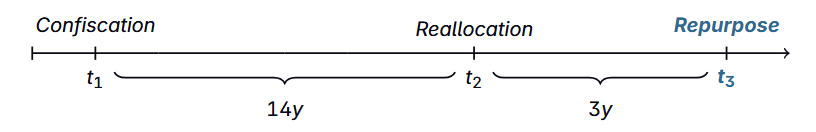
\includegraphics[scale=0.85]{pictures_1/timeline_treatment.png}
    \centering\caption{The CRR policy timeline.}
    \label{fig:jmp_crr_timeline}
    \end{center}
    \end{figure}
    
  \vspace{0.4cm}
Figure~\ref{fig:jmp_policy_counts} shows the number of confiscated, reallocated, and repurposed properties in the historically Mafia-ridden municipalities in my sample. Confiscations and reallocations begin rising from the 1990s, while repurposing practices, first established in the late 1990s, increase dramatically in the late 2010s. On average, it takes 14 years for confiscated Mafia properties to be effectively reallocated, and a further 3 years for them to be repurposed once reallocated. \\
This paper focuses on the final stage of the CRR policy. While existing work shows that the reallocation of Mafia properties affects economic outcomes such as housing prices and market concentration \citep{boeri_localized_2023, ferrante_shall_2021}, a main gap remains: the study of the socio-economic effects of the repurpose of these properties \citep{ferrante_mafia_2021}. The administrative transfer from the ANBSC to local authorities may signal the removal of Mafia control, but it does not by itself constitute a tangible renewal of the local social fabric \citep{falcone_beneitalia_2016}; that renewal occurs only at the repurpose stage. The staggered timing between reallocation and repurpose allows me to disentangle the two effects and assess whether the effects I measure are driven by the reallocation of properties or by their active repurposing. I exploit this timing directly in Section~\ref{sec:jmp_results}, where I show that reallocation alone has no effect on dropout while the repurpose does. \par
 
  
  \begin{figure}[htbp]
  \begin{center}
    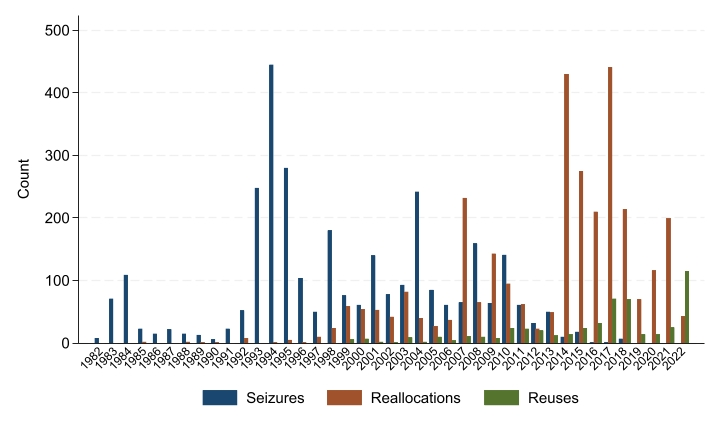
\includegraphics[scale=0.9]{pictures_1/instit_back_graph.jpg}
    \centering\caption{Number of confiscations, reallocations and repurposes from 1982 to 2022.}
    \label{fig:jmp_policy_counts}
    \end{center}
    \end{figure}
\vspace{0.2cm}
 
 %%%%% The figure shows the distribution of mafia assets. the changes are exogenous --> put a graph with 3 lines like mcaiela sviatschi in affecting the surrounding area. dovrei mettere forse anche mafia presence? we see, magari mafia crimes (1) e mafia perception (2) puo essere anche a livello Nazionale, giusto per dare un'idea , non lo so sulla mafia ci pensero'



 Having established that the repurpose of properties is the stage at which the intervention becomes tangible, I follow describing what the repurpose involves and why it is likely to affect young people in particular.\par
 Once repurpose of social use, the property previously owned by the Mafia families transforms into public spaces and community centres managed by local NGOs. These spaces serve as hubs for social activities, youth programs, and community development initiatives, involving direct citizen participation by promoting trust, social cohesion, and sustainable local development \citep{nazzaro_il_2021, falcone_beneitalia_2016}. Residents of all ages participate in recreational and educational activities aimed at reclaiming neighbourhood spaces, rebuilding social bonds, and fostering anti-Mafia resilience. The properties hold particular educational significance as centres that represent safe spaces for young people during after-school hours and weekends, with participants often sharing their positive experiences in schools and throughout the wider community \citep{nazzaro_il_2021}. The transformative power of the repurpose practices is perhaps most strikingly demonstrated by the behaviour of Mafia affiliates, as they frequently attempt to occupy or vandalise their former properties, revealing their deep concerns about the potential for these spaces to start serving as community assets \citep{italian_ministry_of_justice_carta_2018}.


%%%%%%%%%%%%%%%%%%%%%%%%%%%%%%%%%%%%%%%%%%%%%%%%%%%%%%%%%%%%%%%%%%%%%%%
%%%%%%%%%%%%%%%%%%% THEORETICAL FRAMEWORK %%%%%%%%%%%%%%%%%%%%%%%%%%
%%%%%%%%%%%%%%%%%%%%%%%%%%%%%%%%%%%%%%%%%%%%%%%%%%%%%%%%%%%%%%%%%%%%%%
\FloatBarrier
\vspace{0.6cm}
\section{Conceptual framework}
\label{sec:jmp_conc_framework}
In this section, I develop the conceptual framework motivating my empirical analysis. I first draw on the opportunity cost framework from the economics of crime literature to explain how Mafia presence shapes juveniles' educational incentives, particularly in historically Mafia-ridden neighbourhoods. I then review the existing evidence on how Mafia groups leverage their properties to sustain juvenile recruitment and establish alternative authority structures. Finally, I introduce the potential channels through which the repurpose of Mafia properties can affect juveniles trajectories. Rather than presenting formal model predictions, this section aims to motivate the economic mechanisms underlying the estimated treatment effects. \par
\medskip
Building on the literature  about the trade-off between crime and education \citep{lochner_education_2004, lochner_non-production_2011, lochner_effect_2004, machin_crime_2004}, which extends the work from \citet{becker_crime_1968}, I discuss how students weigh their propensity to invest in education against joining Mafia networks. This trade-off depends on the balance between two options at critical educational junctures: the legitimate pathway offered by accumulating human capital and the alternative pathway offered by the Mafia. Each carries its own costs and returns, which are shaped both by the local opportunity structure and by the updated beliefs about the Mafia and the State. I argue that the repurpose of Mafia properties creates a local shock to the perception of the Mafia and the State, altering the opportunity cost of this trade-off in favour of education. \\

On the one hand, juveniles weigh the costs and benefits of joining the Mafia. The costs relate to the probability of being arrested and the related punishment, while returns not only relate to monetary gains, but also to non-monetary benefits such as local power, reputation, and social status, which are essential for the Mafia to maintain territorial and social control \citep{gambetta_sicilian_1993, sciarrone_il_1998}. Indeed, young people living in areas dominated by the Mafia often view the Mafia as a fast and viable path to success, with powerful bosses serving as role models \citep{caglayan_organized_2017}. This is reinforced where family and kinship ties bind households to criminal organizations: Mafia groups are deeply rooted in local social networks \citep{sciarrone_il_1998}, and growing up in a family or community with existing criminal connections exposes juveniles to affiliation as an everyday, normalised life trajectory rather than an unlikely choice \citep{sviatschi_making_2022}.


On the other hand, the same juveniles consider the returns to education against its costs. Because the returns to schooling operate largely through the future gain of higher legitimate wages, they are inseparable from the opportunity cost of crime. The absence of legitimate labour market opportunities play a role in shaping the opportunity cost of joining the Mafia. Since human capital raises the opportunity cost of unskilled, street-level crime through foregone earnings \citep{lochner_education_2004}, juveniles with the weakest labour market prospects have the least to lose from Mafia affiliation; consistent with this, falls in wages at the bottom of the wage distribution have been shown to directly increase crime \citep{machin_crime_2004}. For juveniles growing up in poverty, the income and status that Mafia affiliation promises represent one visible routes to social mobility, as vividly depicted in the several towns around Naples \citet{balestrini_sandokan_2004}. In that context, Mafia affiliation might appear as a reliable pathway for career advancement \citep{catozzella_alveare_2011}.  \par
\medskip
 Through what mechanism does the repurpose of such properties weakens the social influence of Mafia networks? The effect is likely to operate through several channels, which I test and discuss in greater detail in Section~\ref{sec:jmp_mechanisms}.
First, anti-Mafia policies can alter the cost-benefit calculation of joining the Mafia by updating juveniles beliefs. Since Mafia strength relies heavily on social consensus, civil society interventions can effectively erode this accumulated power \citep{arlacchi_palude_1987}. Repurposing confiscated properties for social activities directly targets one of the key functions these assets serve within Mafia organisation: that of \emph{positional goods}, namely visible symbols of territorial control and legitimacy \citep{hirsch_social_1976, baldascino_gestione_2012}. By acting as tangible manifestations of power and wealth, these properties help Mafia families to project authority and maintain their role model status within local communities \citep{mosca_social_2017}. The conversion of Mafia properties into community spaces can lower the return to criminality by undermining the Mafia's capacity to present itself as a legitimate and aspirational force. In the same way, by displacing the Mafia as the salient model of local success, the policy may raise the perceived returns to education, making meritocratic advancement more visible as a viable route to status. \\
Second, juveniles may update their beliefs about the State's capacity to confront the Mafia. A confiscated property visibly and durably repurposed for public use is a credible signal that the State can confiscate criminal assets and repurpose them for collective use, a more demanding demonstration of enforcement than arrest alone \citep{chiodo_community_2021, mosca_social_2017, heller_thinking_2017}. As trust in institutional capacity rises, juveniles might perceive a higher expected cost of Mafia affiliation, facing what appears to be a stronger and more present State.
 \\
Last, the repurpose of properties may reshape the local opportunity structure. First, confiscations accompany the arrest of Mafia families, reducing both their capacity to recruit juveniles locally and the criminal earnings they can offer, lowering the material returns to Mafia affiliation. Second, repurposed properties that deliver education-oriented activities can provide direct support that keep juveniles in school throughout critical educational junctures, lowering the effective cost of staying enrolled \citep{heller_summer_2014, garcia_early_2019}. Third, properties repurposed for cultural and social use can represent additional local amenities that engage youth, while signalling visible urban regeneration \citep{datcher_effects_1982, ludwig_long-term_2013}. Together, these channels might contribute to raise the cost of joining the Mafia and lower the cost of investing in education. \\
These channels carry distinct empirical features, which Section~\ref{sec:jmp_mechanisms} exploits to separate them. If the effect operated by lowering the material returns to affiliation through reduced recruitment capacity, it should emerge at confiscation, when the family is removed, rather than at the time of repurposing. If it operated by lowering the cost of remaining in education through additional support provided, it should be concentrated in properties delivering education-oriented activities and should be visible in academic attainment as well as in enrolment. If it operated through generic amenity provision or neighbourhood upgrading, it should not depend on the property's criminal origin and should vary with local property values. The belief-based channels, by contrast, act on the perceived rather than the realised terms of the trade-off: they predict effects concentrated in properties that were most visibly symbolic of Mafia authority, emerging only once repurposing is complete and community activities are established, and accompanied by measurable shifts in how juveniles assess the relative standing of the Mafia and the State. The effects I estimates are with the perceived cost of affiliation rising first as the State's capacity becomes visible, and the perceived return to the criminal pathway eroding as that perception takes hold.


%%%%%%%%%%%%%%%%%%%%%%% DATA %%%%%%%%%%%%%%%%%%%%%%%%%
\FloatBarrier
\section{Data}
\label{sec:jmp_data}
\FloatBarrier
\subsection{Schools data}
\label{sec:jmp_schools_data}
 I use school-level data covering the public upper secondary schools in the major Italian urban areas with significant historical Mafia presence.  School-level data were provided by the Italian Ministry of Education, allowing me to geocode each specific school's location to cover the period from 2015 to 2022. The data present information about the number of students completing each academic year in each grade, graduating at the end of the educational cycle, as well as their age and gender. Additionally, the data provide information about the school-specific educational track: \emph{Licei} or Academic High Schools focus on academic subjects and mainly prepare students to enrol in tertiary education, \emph{Istituti Tecnici} or Technical High Schools provide a more practical and technical education, while \emph{Istituti Professionali} or Vocational High Schools offer vocational training. From each track, we know students can specialise in different subjects; the specialisations offered to date count to 14 and are summarised in Table~\ref{tab:jmp_hs_tracks}, as outlined by the Italian Ministry of Education\footnote{The organisation of Italian high schools can be found online on the website of the \citet{ministry_of_education_scuola_2024}: \href{https://www.mim.gov.it/web/guest/scuola-secondaria-di-secondo-grado}{Organisation of upper secondary education in Italy}.}. The universe of possible high school tracks is described in more detail in Figure~\ref{fig:school_types}. To provide clarity to the analysis, I first omit schools that changed address across the years, unless they were relocated within the same specific census block\footnote{As explained later in this Section, since the treatment is defined by aggregating census blocks into schools' catchment areas, any change of the school's location occurring within the same census block is insignificantly affecting my identification strategy.}. Second, to reduce measurement error, I double-check that schools that merged at some point in the panel were located at the same address.
Last, I exclude from my sample private high schools, which in the Italian context target a specific subgroup of the population and only represent 5\% of the entire country's enrollment preferences \citep{istat_istruzione_2021}. 

% Table generated by Excel2LaTeX from sheet 'Sheet1'
\begin{table}[H]
\caption{Types of high school tracks in the Italian educational system.}
\label{tab:jmp_hs_tracks}
\vspace{0.2cm}
\centering
\scalebox{0.78}{
 
\begin{tabular}{p{9.22em}p{19.5em}rr}
    \textbf{HS Tracks} & \textbf{Description} & \textbf{Specialisations} & \textbf{Sample \%} \\
    \midrule
        \textit{Academic} & Provide students with the skills and knowledge for higher education in classical studies, scientific studies, linguistic studies, humanities, music, and fine arts. & 6 & 0.411 \\
    \textit{Technical} & Provide practical and technical skills related to key sectors such as administration, marketing, and industrial development. & 2 & 0.371 \\
    \textit{Vocational} & Provide vocational skills for industrial, commercial, and social development, as well as agricultural, maritime and hospitality skills. & 6 & 0.101 \\
\end{tabular}
    }
\end{table}
\vspace{0.5cm}


Italian upper-secondary schools offer a five-year educational program spanning from grade 9 to grade 13. Students typically complete grade 9 in their first year at the age of 14 or 15, and graduate at grade 13 when they are 18 or 19, respectively. The Italian academic year begins in September, with all students born in the same calendar year enrolling together regardless of their month of birth. However, the successful completion of each academic year is measured in May. Figure~\ref{fig:jmp_age_grade} illustrates the expected age of enrolled students measured at the end of each academic year. Students born between January and May will be 15 years old when they complete grade 9 and 19 years old at the time of graduation, while those born between June and December will be 14 when they complete grade 9, and 18 years old at the time of graduation \footnote{Each academic year starts in September and students born in the same calendar year get enrolled regardless their month of birth. The number of students who completed each academic year is measured in May.}.
\vspace{0.3cm}

  
  \begin{figure}[H]
  \begin{center}
    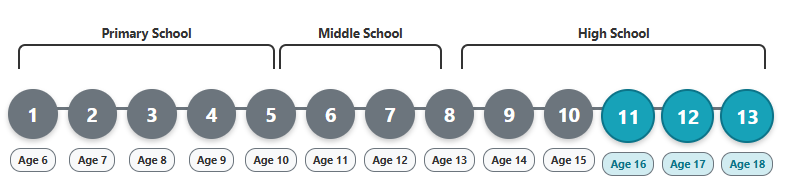
\includegraphics[scale=0.9]{pictures_1/Screenshot 2026-01-29 155329 (1).png}
    \centering\caption{The timeline of compulsory schooling in the Italian educational system. This Figure represents the scenario where students do not start school later and do not repeat any year.}
    \label{fig:jmp_age_grade}
    \end{center}
    \end{figure}


Compulsory education lasts 10 years, from ages 6 to 16, creating a critical threshold for school attendance. Before the age of 16, students have limited discretion, making dropouts very rare\footnote{In Italy, Law 296/2006 extended compulsory education from ages 6–15 to 6–16 and raised the minimum working age accordingly. Compliance is overseen by local authorities under Legislative Decree 297/1994: mayors track enrollment, identify non-attending students, and issue warnings, with persistent violations leading to legal action. As a result, leaving school before 16 is both legally prohibited and actively monitored, making it very unlikely for students to not attend school before turning 16 without facing institutional scrutiny within an entire academic year.}. However, once students turn 16, they gain legal freedom to discontinue their studies. This legal framework leads to specific dropout patterns, which typically happen in the transition between the third and the fourth year of the upper secondary cycle, namely from grade 11 to grade 12. Indeed, as shown in Figure~\ref{fig:jmp_age_grade}, after completing grade 11, all students are at least 16 years old. Exhisting empirical evidence support this pattern: in 2015, the Italian average rate of students dropping out from high schools before turning 16 was only 3.3\%, while the rate of students who dropped out after turning 16 was 8.2\%. Similar patterns persist over time: in 2022, just 2\% of the students dropped out before turning 16, compared to 5.41\% who dropped out after reaching this age threshold \citep{istat_dispersione_2023}. This paper focuses on the dropout behaviour after grade 11 has been completed, specifically when all students are 16 or older and have gained the legal autonomy to discontinue their education. Educational decisions at this juncture are particularly sensitive to contextual influences, as students weigh the costs and benefits of continued schooling against immediate alternatives \citep{angrist_does_1991}. This is precisely when local environmental factors exert their strongest influence on educational persistence \citep{oreopoulos_compelling_2006}. Transforming former Mafia properties into educational or community resources is likely to reshape students’ attitudes and beliefs during this formative stage, allowing me to distinguish the effects of reuse practices from the constraints imposed by earlier compulsory schooling. \par
\medskip

The main outcome variable is the cumulative dropout rate among students aged 16 and older, calculated by tracking the same cohorts over time. I focus on transitions between grades 11 and 13, since this is when students typically turn 16 or older. The measure of dropout is built as follows: I track the number of students who completed grades 11, 12 and 13 in year $t-1$ and measure how many of them completed grades 12 and 13 in year $t$. From this, I subtract those who graduated after completing grade 13 in time $t$. The remainder is then calculated as the share of the baseline cohort of students who completed grades 11, 12 and 13 in year $t-1$.\footnote{Dropout in the final year, namely grade 13, is quantitatively negligible, as students who reach this stage have already demonstrated sustained persistence and are unlikely to leave before graduation. An additional concern is that this measure may capture exam-related attrition as students who complete grade 12 but fail or choose not to sit the final exam. To address both concerns, in Figure~\ref{fig:es_excl_g13_} I re-estimate the main specification using an alternative dropout measure that tracks only whether students who completed grade 11 in year $t$-1 subsequently enrol in grade 12 in year $t$, and whether students who completed grade 12 in year $t$-1 subsequently enroll in grade 13 in year $t$. This way the measure only captures the decision to continue or abandon schooling at each grade transition, without conflating voluntary dropout with failure to complete the final high-school examination.} This share tells me how many students from the same cohorts successfully enroll in the following years after turning 16. The cumulative dropout measure is defined as follows:
\par
\vspace{0.3cm}
\begin{equation}
D_{g11-13{_{ct}}} = \frac{C_{g11-13_{ct-1}} - G_{g13_{ct}} - C_{g12-13_{ct}}}{C_{g11-13_{ct-1}}}
\end{equation}
\vspace{0.3cm}

where $D_{g11-13}$ represents the cumulative dropout rate for students aged 16 or above in year $t$ for school catchment area $c$, $C_{g11-13}$ represents the number of students enrolled in grades from 11 to 13 in year $t-1$, $G_{g13}$ is the number of students who completed grade 13 and therefore graduated in year $t$, and $C_{g12-13}$ represents the number of students from the same cohorts who remain enrolled in grades 12 and 13 in year $t$. This approach ensures, by construction, that dropout rates reflect genuine dropout patterns from the same cohorts of students rather than demographic changes between different cohorts. By isolating graduation as a separate category, the measure also provides an accurate assessment of educational dropout that distinguishes between students who leave due to the successful completion of the five-year program versus those who drop out before finishing their studies. Moreover, to address the concern of students' migration and internal retention for grades 11, 12 and 13, I show in Section~\ref{sec:jmp_empirical} that my results are robust while controlling for these factors. It is possible that students born between January and May turn 16 during grade 11 and drop out before its completion, meaning they would not be captured by my main outcome measure. This could lead to a downward bias, causing me to underestimate the true effect of the policy on dropout rates. However, Section~\ref{sec:jmp_results} addresses this concern directly by estimating the effect of the policy on dropout rates across grades 10 to 13, thereby including these students. The results remain unchanged, suggesting that this source of bias is negligible in practice. Another concern is that changes in enrollment between grades 11 and 13 may partly reflect students transferring to another school rather than genuinely dropping out. However, the Italian Ministry of Education (2017) show that schools' transfers and other motivated exits account for only 6.4\% of all student departures from upper secondary school, while 89.1\% represent genuine unmotivated abandonment. This suggests that school transfers constitute a quantitatively minor component of enrollment changes, and that controlling for retention rates at grades 11 and 12, which absorbs the main driver of mobility, makes the estimated effects more plausibly reflect genuine decisions to discontinue education.  \par



\FloatBarrier
\subsection{Mafia properties data}
\label{sec:jmp_mafia_data}
I create a novel database covering the universe of reused Mafia properties by scraping various institutional sources and collaborating with the Italian Antimafia Association \emph{Libera}. The data collection represents a novel contribution to the literature, addressing previously fragmented sources that have never been systematically compiled and employed for empirical analysis. \\
I start the dataset construction from the list of reallocated Mafia properties released online by the \citet{anbsc_beni_2023}. The data comprise a unique identifier for each Mafia property, the type of real estate, its usage before confiscation, the recipient and purpose of the reallocation, and the dates of confiscation and reallocation. 
I was able to geocode 3119 of the total count of 3667 Mafia properties \footnote{The majority of the properties which I failed to geocode due to incomplete information represents lands in rural areas, which will less likely affect the dropout rates of the urban areas I investigate.}, with 42\% and 41\% of them being reallocated for social and institutional purposes, respectively. Crucially for my analysis, 66\% of the properties have been reallocated to the jurisdiction of the nearest municipality, as only these properties can undergo the full transformation from confiscated Mafia properties to community resources. Finally, 83\% of the reused properties are identified as housing estate - such as villas and flats - while the 10\% consists of commercial and industrial estate, and the 12\% of lands. Additional information about the attributes of repurposed properties which have been effectively repurposed is reported in Appendix~\ref{sec:jmp_app_B}. \par
Second, I scrape information from the website \emph{\href{https://www.confiscatibene.it/}{Confiscatibene}}, which is managed by the Association \emph{Libera} in collaboration with the ANBSC. On this platform, both \emph{Libera} and several users update the current state of the properties, flagging whether they have been reused for any social activity. Additional information are provided about the description of the activities, and the name of the local NGO managing the property. In a few cases, the website also reports the year and the month when the reuse experience started. Since the website releases reuse-related information up to 2018, I collaborated with the \emph{Libera} national managers of confiscated Mafia properties, who allowed me access to their yearly survey targeting the NGOs managing reused Mafia properties, giving me additional information about the reuse practices to date. Finally, to minimise missing information, I cross-referenced my data with the information shared by every single municipality about the current status of Mafia properties under their jurisdiction. \footnote{According to the Art. 48 of the Antimafia Code (2011), municipalities are obliged to address trasparency regarding the management of Mafia properties under their jurisdiction, and they are expected to share a monthly updated list of the properties and their current state of use. Data limitations imply that it is possible to have some missing information about some repurposed properties from municipal archives and \emph{Libera's} website, implying that my measure of reused Mafia properties would likely be an undercount. Any resulting attenuation bias would suggest my estimates represent a lower bound of the true effect.}. Table~\ref{tab:census_data} reports several attributes of the local context where these properties have been repurposed, including population characteristics, educational attainment, labour market conditions, and area-specific features such as real estate conditions and the presence of NGOs. Moreover, Figure~\ref{fig:jmp_assets_map} shows the spatial distribution of Mafia real estate in the ten urban areas which I investigate in this paper. Between 2015 and 2022, 346 of the 3119 Mafia properties were reused for social purposes by municipalities and local NGOs, with the majority in the largest municipalities, such as Palermo and Naples. \par
To identify and analyse the types of social activities organised at each site, I manually categorise the repurposing activities based on the labels provided by previous reports published by \emph{Libera} \citep{falcone_beneitalia_2016}. I identify five primary types of activities: educational, welfare, cultural, employment-related, and other. Figure~\ref{fig:jmp_wordcloud} presents a word cloud of the 100 most frequent words appearing in the descriptions of the activities, offering a qualitative overview of the most common themes. Figure~\ref{fig:jmp_repurpose_cats} presents the frequency distribution of each mutually exclusive activity category, illustrating the relative prevalence of each type of social reuse across the sample. Table~\ref{tab:jmp_reuse_activities} provides a detailed description of each category, outlining the defining characteristics and representative examples of the activities classified within them. 
     \begin{figure}[H]
  \begin{center}
    
\includegraphics[scale=0.65]{pictures_1/wordcloud2.png}
    \centering\caption{Word cloud of the descriptions of activities in reused Mafia properties illustrating the 100 most common terms used.}
    \label{fig:jmp_wordcloud}
    \end{center}
    \end{figure}

        \begin{figure}[H]
  \begin{center}
    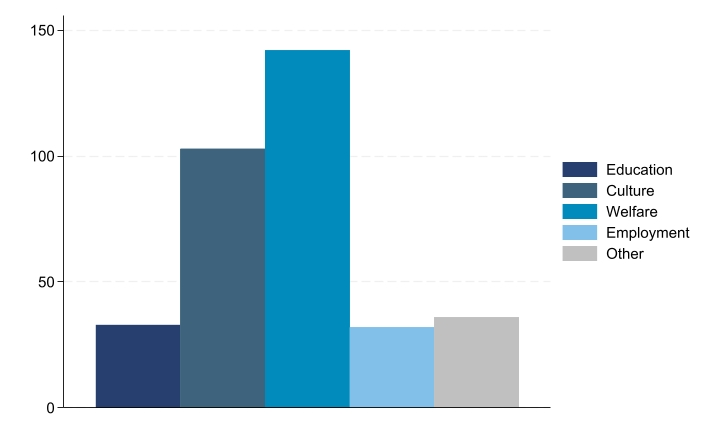
\includegraphics[scale=0.8]{pictures_1/primarycat_repurposed.jpg}
    \centering\caption{Repurpose categories of activities.}
    \label{fig:jmp_repurpose_cats}
    \end{center}
    \end{figure}
    
\begin{table}[H]
\caption{Types of reuse activities described.}
\label{tab:jmp_reuse_activities}
\vspace{0.2cm}
\centering
\scalebox{0.78}{
    \begin{tabular}{lrp{16.93em}r}
    \textbf{Activity} &       & \multicolumn{1}{l}{\textbf{Description}} & \multicolumn{1}{l}{\textbf{Reused Mafia properties \%}} \\
    \midrule
    Education &       & After-school activities and schooling support, socio-educational activities for at-risk juveniles & 9.5\% \\
     Culture &       & Cultural activities to raise awareness about organised crime, the rule of law and self-responsibility & 29.8\% \\
    Welfare &       & Places for housing emergency, activities to assist the homeless and people in need, social activities targeting  vulnerable groups & 41.1\% \\
    Employment &       & Support and training activities for unemployed people or fragile groups & 9.2\% \\
    Other  &       & Activities in the agricultural industries aiming to sell organic products and other & 8.9\% \\
    \end{tabular}%
}
\end{table}

% Table X summarises the number of Mafia real estate for each categories and gives a comprehensive description of the categories' labels itself.

\FloatBarrier
\subsection{Treatment allocation}
\vspace{-0.19cm}
\label{sec:jmp_treatment}
Given the localised nature of the analysis, it is necessary to identify which students attend which school by linking their residential addresses and the schools' locations. To address this issue, I would need to employ student-level educational data, which are not easily released to the public. To systematically assign students to schools in the absence of formally defined school districts - a common challenge while using educational data - I build school catchment areas using an adapted distance-based location-allocation method. My approach follows established practices in the spatial economics analysis for defining catchment areas when administrative boundaries are unavailable \citep{pearce_techniques_2000, singleton_estimating_2011}. The main approaches to address this issue are either the use of weighted-Voronoi polygons, which address this issue from a geometric perspective, or the location-allocation method, which frames the problem in terms of student demand, based on the students' residential distribution, and school supply. \citet{pearce_techniques_2000} shows that while the former offers computational simplicity, the latter performs better in predicting the dimensions of schools' catchment areas in real-world applications. \par
I construct school catchment areas following the location-allocation method in three main steps: first, I consider the Euclidean distance between each school and each residential census block to select the closest schools for each of them, which is the main factor influencing enrollment preferences \citep{mandic_enrolling_2017}. The geometry of each census blocks is obtained from the 2011 Italian census data \citep{istat_censimento_2011}. Second, I differentiate catchment areas by educational specialisation sub-track, acknowledging that families' and students' choices also depend on the type of track offered and preferred. I ultimately created catchment areas for 14 distinct sub-tracks that map onto the three main tracks described in Table~\ref{tab:jmp_hs_tracks}. Rather than imposing arbitrary distance constraints, the sub-track-specific assignment approach naturally determines appropriate catchment boundaries by ensuring each census block is matched to its nearest school within each educational specialisation. This method avoids the problem of unassigned blocks while acknowledging that students' choices are defined by program availability rather than arbitrary distance thresholds. 
I work with a total of 10556 census blocks, with an average area of 0.05 square kilometres, an average population of 200 individuals, of which 11.64\% is aged 14 to 19. I compute 334 schools' catchment areas aggregating on average 580 census blocks per school \footnote{Because catchment areas are calculated for each school sub-track, the census blocks sum up only within each sub-track and not across the entire dataset.}. Each catchment area has an average population of around ten thousand individuals,  with 570 individuals aged between 14 and 19 years old. Additionally, I construct a second set of school catchment areas where I account for the baseline number of students enrolled in each school. This approach captures the fact that students’ allocation to schools depends not only on geographic proximity but also on school capacity. Appendix~\ref{sec:jmp_app_D} provides the details of this procedure, while Section~\ref{sec:jmp_results} presents the results according to this alternative construction method. \par
\medskip
To define treated schools' catchment areas, I employ the precise address of each repurposed Mafia property, and I compute two main treatment measures: first, to investigate the extensive margin of the treatment, I create a dummy variable which is equal to 1 whenever at least one Mafia property has been repurposed within the boundaries of the school catchment area in a specific year. Areas which have been treated before the beginning of the panel are coded as always treated. Second, I compute an intensive margin measure as the count of the properties reused for each catchment area in each specific year;  this measure provides a continuous treatment intensity measure that varies both spatially and temporally. To better control for demographic confounders, I additionally compute area-specific weights based on the local student population. As a roubstness check, I weight each catchment by the average distance of repurposed properties from the population-weighted centroids of each school catchment area \footnote{Population-weighted centroids are calculated by taking the weighted average of the coordinates of all census block centroids within each catchment, where the weights are the high school-age population (ages 14-19) in each block, resulting in a single centroid per catchment that reflects the spatial distribution of the residential student population}. These weighted measures capture both the localised nature of property reuse and the expected decay in its effect with distance from the treated sites \citep{boeri_localized_2023, damm_does_2014}. \\
Figure~\ref{fig:jmp_catchment_example} provides an ad-hoc example of how the catchment areas for each school track are computed. Each school, shown as a filled coloured circle, is assigned a set of census blocks based on the Euclidean distance between the blocks’ centroids (grey dots) and each school. Each block is assigned to the nearest school for its specific school sub-track. The colored regions represent the resulting schools' catchment areas: School A (blue), School B (green), and School C (orange). The grey lines connecting each census block to its assigned school represent the relative Euclidean distance and allow to visualise the distance-based assignments. Figure~\ref{fig:jmp_catchment_example} also shows the presence of repurposed Mafia properties within the catchment areas for a specific year, marked by the purple diamonds. School A serves as  \emph{control}, while Schools B and C are \emph{treated} under the extensive margin of the treatment; notably, Schools B and C differ in treatment intensity, as two properties are reused within School C’s catchment area, whereas only one property is reused within School B’s catchment area. 

\medskip
 \begin{figure}[H]
  \begin{center}
    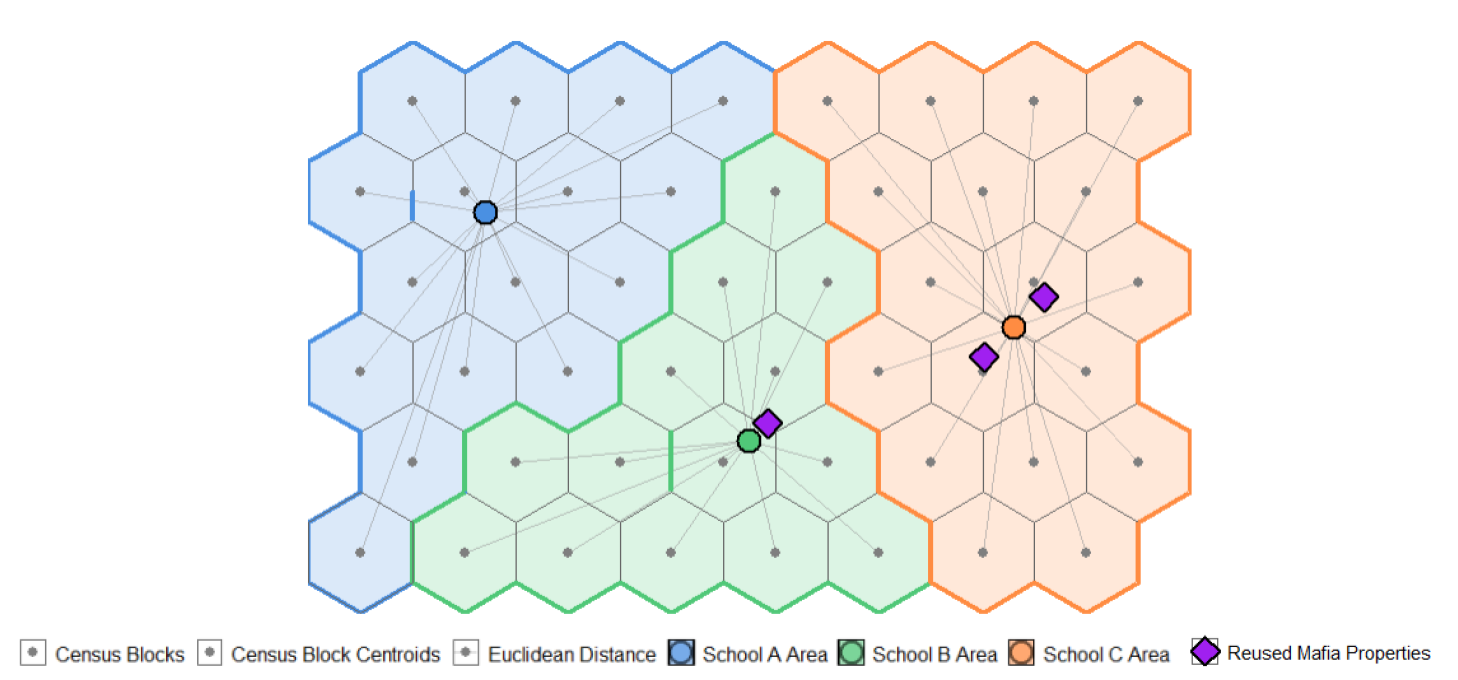
\includegraphics[scale=0.5]{pictures_1/exagons_treatmentall.png}
    \centering\caption{Ad-hoc example of schools' catchment areas construction.}
    \label{fig:jmp_catchment_example}
    \end{center}
    \end{figure}
    \vspace{-0.2cm}
\FloatBarrier
\subsection{Survey on youth's perception of the Mafia}
\label{sec:jmp_survey}
I employ survey data from the  \emph{Survey of the Perception of the Mafia} to investigate changes in the perception of the Mafia, the State, and their role in shaping youth's attitudes. The survey data are created and provided by the Sicilian NGO \citet{centro_studi_pio_la_torre_survey_2025}, targeting students enrolled from grade 11 to grade 13, roughly aged between 16 and 19. Some responses are aggregated at the school level, which I can identify with a unique code, while others provide a unique identifier per respondent. The survey, which spans from 2009 to 2024, is administered to students by the teachers thanks to a collaboration between the schools and the NGO. While this creates a selected sample, it allows me to directly test whether changes in the perception of the Mafia serve as a mediating channel for the treatment effect\footnote{Results reported in Section~\ref{sec:jmp_mechanisms} also account for the baseline measure of students' socio-economic background to address any related concern.}. For this purpose, I focus on the answers collected from 2011 to 2022, a time frame for which consistent questions can be examined. \par
The students' questionnaire comprises a battery of questions focusing on several key dimensions of the perception of the Mafia and the State: the students' beliefs about whether the Mafia could be useful or not for career advancement, their perception of Mafia' strength and State's strength, their trust in several public institutional figures, student-level definitions of the Mafia, and questions about how their family perceives the Mafia.
Table~\ref{tab:survey_questions} offers a complete list of the answers I employ. For multiple-choice questions, I construct a dummy variable for each response option, such that the dummies sum to the total number of responses. For agreement scales, I use the top and bottom of the distribution to capture strong agreement and strong disagreement with each statement. For the student-level answers, I perform a simple text analysis and calculate sentiment scores for the words used by the students to describe the Mafia, which is further discussed in Section~\ref{sec:jmp_mechanisms}. I use these indicators to assess whether the reuse of Mafia properties leads students to change their perception and sentiments towards the Mafia and educational investments.  



 
\FloatBarrier
\subsection{Other data}
\label{sec:jmp_other_data}
 I collect information about the socio-economic conditions of the local community around the schools; understanding these contextual factors is crucial, as community socio-economic conditions can affect educational outcomes through multiple pathways. \par
I first collected information about rental prices from 2016 to 2022 from \href{https://www.immobiliare.it/}{Immobiliare.it} as a proxy for deprivation at the neighbourhood level; second, from the \href{https://servizi.lavoro.gov.it/runts/it-it/}{National Registry of the Third Sector}\footnote{The registry is offered online by the Italian Ministry of Labour and Social Policies (MLPS)}, I scraped information about local NGOs, such as their legal address, the time the NGOs were created, the type of activity they pursue and the number of people which engage in their activities. As with the Mafia properties, I geocode the NGOs' addresses to map them at the street level. Moreover, I digitise on GIS the historical maps about the neighbourhood-level distribution of Mafia families in Italy published by the Italian Antimafia Directorate \citet{dia_relazione_2015-1, dia_relazione_2015}. Last, I employ the educational data as described in Section~\ref{sec:jmp_schools_data} to construct proxies for student migration and grade retention at the school level. I define student migration as the average annual rate of students who do not complete the grades 9 and 10, typically aged between 13 and 15. This variable captures students who leave the school where they first enrolled before turning 16, when they are unlikely to be dropping out of the educational system and are more likely to transfer to another institution. I define grade retention as the share of students who complete grades 11 and 12 being older than the expected age for their grade cohort, indicating they have repeated a grade or experienced delayed academic progression. Controlling for both student migration and grade retention is essential, as these factors can directly affect dropout rates and may be correlated with changes in school catchment areas, potentially biasing the estimated effects. Appendix~\ref{sec:jmp_app_D} presents how these measures are built in more detail. \par
\medskip
Table~\ref{tab:jmp_desc_stats} shows descriptive statistics of the observable socioeconomic attributes for both treated and control areas measured at the baseline, before the reuse of any Mafia property occurs. First, treated and control areas exhibit virtually identical baseline educational outcomes, both in terms of students' migration and grade retention, which supports the validity of using dropout rates as the primary outcome measure in this specific setting. Moreover, treated areas show higher historical Mafia presence, which is expected given that this intervention specifically targets areas with confiscated Mafia properties. These areas also exhibit greater NGO activity and marginally lower rental prices, suggesting they might represent working-class neighbourhoods where both criminal organisations and civil society have historically been active. Because the reuse of properties may be influenced by the local availability of NGOs, I further examine whether pre-existing NGOs' presence is associated with future dropout patterns in Section~\ref{sec:jmp_mechanisms}. I report that NGO activity measured at times $t$, $t-1$, $t-2$, and $t-3$ shows no systematic relationship with subsequent dropout rates, indicating that the baseline NGO presence is unlikely to drive the estimated effects. Crucially, once standard errors are clustered at the school level to account for spatial autocorrelation, any baseline difference loses statistical significance, indicating that treated and control areas are virtually comparable across all the observed dimensions.


\begin{table}[H]
\caption{Descriptive statistics.}
\label{tab:jmp_desc_stats}
\vspace{0.2cm}
\centering
\scalebox{0.7}{
    \begin{tabular}{p{10.11em}lllllllll}
    \toprule
    \multicolumn{1}{r}{} & \multicolumn{7}{c}{\textbf{Reused Mafia property in the school's area}} &       &  \\
    \multicolumn{1}{l}{} & \multicolumn{3}{c}{\textbf{No}} & \multicolumn{3}{c}{\textbf{Yes}} &       & \multicolumn{2}{c}{$\Delta$} \\
    \multicolumn{1}{l}{\textit{Baseline covariates}} & \multicolumn{1}{c}{N} & \multicolumn{1}{c}{mean} & \multicolumn{1}{c}{sd} & \multicolumn{1}{c}{N} & \multicolumn{1}{c}{mean} & \multicolumn{1}{c}{sd} & \multicolumn{1}{c|}{} & \multicolumn{1}{c}{Robust SE} & \multicolumn{1}{c}{Clustered SE} \\
    \multicolumn{1}{l}{} & \multicolumn{1}{c}{} & \multicolumn{1}{c}{} & \multicolumn{1}{c}{} & \multicolumn{1}{c}{} & \multicolumn{1}{c}{} & \multicolumn{1}{c}{} & \multicolumn{1}{c|}{} &       &  \\
    \multicolumn{1}{l}{Mafia presence} & \multicolumn{1}{c}{573} & \multicolumn{1}{c}{0.644} & \multicolumn{1}{c}{0.479} & \multicolumn{1}{c}{1,234} & \multicolumn{1}{c}{0.703} & \multicolumn{1}{c}{0.457} & \multicolumn{1}{c|}{} & \multicolumn{1}{c}{-0.059**} & \multicolumn{1}{c}{-0.059} \\
    \multicolumn{1}{r}{} &       &       &       &       &       &       & \multicolumn{1}{c|}{} & \multicolumn{1}{c}{(0.023)} & \multicolumn{1}{c}{(0.061)} \\
    \multicolumn{1}{l}{NGOs presence} & \multicolumn{1}{c}{561} & \multicolumn{1}{c}{37.43} & \multicolumn{1}{c}{54.26} & \multicolumn{1}{c}{1,207} & \multicolumn{1}{c}{45.45} & \multicolumn{1}{c}{83.01} & \multicolumn{1}{c|}{} & \multicolumn{1}{c}{-8.015**} & \multicolumn{1}{c}{-8.015} \\
    \multicolumn{1}{r}{} &       &       &       &       &       &       & \multicolumn{1}{c|}{} & \multicolumn{1}{c}{(3.837)} & \multicolumn{1}{c}{(8.801)} \\
    \multicolumn{1}{l}{Rental prices} & \multicolumn{1}{c}{561} & \multicolumn{1}{c}{7.450} & \multicolumn{1}{c}{2.251} & \multicolumn{1}{c}{1,207} & \multicolumn{1}{c}{7.261} & \multicolumn{1}{c}{1.756} & \multicolumn{1}{c|}{} & \multicolumn{1}{c}{0.189*} & \multicolumn{1}{c}{0.189} \\
    \multicolumn{1}{l}{} & \multicolumn{1}{c}{} & \multicolumn{1}{c}{} & \multicolumn{1}{c}{} & \multicolumn{1}{c}{} & \multicolumn{1}{c}{} & \multicolumn{1}{c}{} & \multicolumn{1}{c|}{} & \multicolumn{1}{c}{(0.098)} & \multicolumn{1}{c}{(0.278)} \\
    \multicolumn{1}{l}{Students' migration} & \multicolumn{1}{c}{556} & \multicolumn{1}{c}{0.355} & \multicolumn{1}{c}{0.0242} & \multicolumn{1}{c}{1,155} & \multicolumn{1}{c}{0.351} & \multicolumn{1}{c}{0.0398} & \multicolumn{1}{c|}{} & \multicolumn{1}{c}{0.003*} & \multicolumn{1}{c}{0.003} \\
    \multicolumn{1}{r}{} &       &       &       &       &       &       & \multicolumn{1}{c|}{} & \multicolumn{1}{c}{(0.002)} & \multicolumn{1}{c}{(0.004)} \\
    \multicolumn{1}{l}{Grade retention 3rd year} & \multicolumn{1}{c}{559} & \multicolumn{1}{c}{0.0248} & \multicolumn{1}{c}{0.0253} & \multicolumn{1}{c}{1,185} & \multicolumn{1}{c}{0.0247} & \multicolumn{1}{c}{0.0303} & \multicolumn{1}{c|}{} & \multicolumn{1}{c}{0.000} & \multicolumn{1}{c}{0.000} \\
    \multicolumn{1}{r}{} &       &       &       &       &       &       & \multicolumn{1}{c|}{} & \multicolumn{1}{c}{(0.001)} & \multicolumn{1}{c}{(0.004)} \\
    \multicolumn{1}{l}{Grade retention 4th year} & \multicolumn{1}{c}{559} & \multicolumn{1}{c}{0.0156} & \multicolumn{1}{c}{0.0158} & \multicolumn{1}{c}{1,190} & \multicolumn{1}{c}{0.0133} & \multicolumn{1}{c}{0.0145} & \multicolumn{1}{c|}{} & \multicolumn{1}{c}{0.002***} & \multicolumn{1}{c}{0.002} \\
    \multicolumn{1}{r}{} &       &       &       &       &       &       & \multicolumn{1}{c|}{} & \multicolumn{1}{c}{(0.001)} & \multicolumn{1}{c}{(0.002)} \\
    \multicolumn{1}{r}{} &       &       &       &       &       &       &       &       &  \\
    \midrule
    \multicolumn{10}{p{53.61em}}{Notes: The last column presents standard errors clustered at the school level.} \\
    \end{tabular}%
}
\end{table}

%%%%%%%%%%%%%%% EMPIRICAL FRAMEWORK %%%%%%%%%%%%%%%%%
\FloatBarrier
\section{Empirical strategy}
\label{sec:jmp_empirical}
Estimating the effect of reusing confiscated Mafia properties on dropout rates is complicated by the involvement of multiple institutional actors in the reuse process. As discussed in Section~\ref{sec:jmp_other_data}, reused properties tend to be located in more deprived areas with higher civil engagement and baseline Mafia presence. Additionally, the presence of NGOs and unobserved municipality-level characteristics may influence reuse decisions. Although baseline differences between treated and control areas become statistically insignificant once standard errors are clustered at the school level, I take a further step by systematically control for the individual determinants of reuse decisions. I demonstrate that, conditional on these factors, the variation in reuse timing and implementation is plausibly uncorrelated with other determinants of dropout dynamics.\footnote{It is still possible that reused Mafia properties differ based on unobserved factors from those that remain unused - such as specific acts of resistance or vandalism, or unobserved municipal political dynamics - which could bias the estimated effects in either direction. If reused properties are systematically located in areas with greater unobserved criminal resistance, political instability, or social tensions that make reuse more contentious, this could lead to underestimation of the true effect by creating additional challenges for educational improvement that are not captured in the analysis; if reused properties are located in areas with stronger unobserved community mobilization or political commitment to anti-Mafia efforts, this would lead to overestimation of the treatment effect.}
As discussed in Section~\ref{sec:jmp_inst_bg}, when a Mafia property is reused for social purposes - becoming a community, after-school facility, or social services centre - it transforms from a symbol of Mafia power into a symbol of community resistance \citep{mosca_social_2017}. These spaces may improve neighbourhood support and educational services while reshaping local perceptions of the Mafia as an alternative career path. Students at critical dropout ages might rationally weigh the expected returns from education versus criminal careers. The potential effects of reuse activities are therefore twofold: reducing dropout rates by increasing returns to education through enhanced services, or by diminishing the perceived attractiveness of criminal careers as symbols of Mafia power become symbols of State authority and community resilience.
My empirical strategy proceeds as follows: First, I identify the socio-economic determinants of Mafia property reuse. Table~\ref{tab:census_data} in Appendix~\ref{sec:jmp_app_B} shows that even including controls and time trends for such determinants, my results hold. Second, I estimate a difference-in-differences model comparing school catchment areas exposed to reuse practices with unexposed areas. Last, I investigate dynamic treatment effects by examining the intensive margin of the treatment. \par
\FloatBarrier
 \subsection{DiD model}
\label{sec:jmp_did_model}
 I estimate a TWFE model under a DiD design with staggered treatment adoption. The first model estimates the extensive margin of the treatment comparing treated and control schools before and after the first Mafia property get reused. I define as \emph{treated} schools catchment areas which have at least one reused Mafia property within their boundaries, and \emph{control} those who do not\footnote{I estimate an additional model where I restrict the sample to the schools which already host at least one reallocated property, to make sure the areas are comparable according to the policy process. Results are reported in Figure~\ref{fig:es_evertreated}.}. The sample comprises a total of 1807 observations with 256 unique school catchment areas for which the dropout information is not missing\footnote{The dropout measure has several missing values for the years 2015 and 2016. The measure tracks students from the same cohorts from grade 11 to graduation after the completion of grade 13. Dropout rates cannot be computed for 2015 cohorts (data for 2014 are not available) and some 2016 cohorts (due to missing data in 2015 preventing complete cohort tracking). Despite this, the staggered policy implementation provides sufficient treatment variation for identification.}; of those, 58 were never treated, while 198 have been treated at some point in the sample. The first model is specified as: \par
\begin{center}
          \begin{equation} \label{1stspec}
        \begin{split}
 Dropout{G11-13_{cnmt}} = \beta_1Repurpose_{ct} +\beta_2X^{'}_{ct}  +\delta_c  + \eta_{t} + \epsilon_{cnmt}
         \end{split}
      \end{equation}
\end{center}
\vspace{0.4cm}
where $DropoutG11-13$ is the share of students dropping out during grade 11 of high school in schools catchment area $c$, neighbourhood $n$, and municipality $m$ measured in time $t$; $Repurpose$ is a binary indicator equal to 1 if there is at least one Mafia property repurposed within the school catchment area in time $t$ and after the first repurpose. Since schools are treated at different points in time, the coefficient of interest $\beta_1$ captures the average treatment effect on treated  (ATT) comparing treated school catchment areas to never or not yet treated ones. $X'$ is a vector of controls at the catchment area level, including migration dynamics and grade retention rates for grades 11 and 12, which account for additional educational disruptions that could be captured by the dropout measure \footnote{I confirm that the treatment does not affect student migration or grade retention, indicating that these controls capture pre-existing school characteristics rather than treatment effects. Results are reported in Table~\ref{tab:jmp_main_controls}.}. Additionally, $\delta_c$ captures the catchment areas fixed effects, and $\eta_{t}$ captures the year fixed effects. Standard errors are clustered at the school catchment area level to account for spatial autocorrelation. \par
 \medskip
As shown in Table~\ref{tab:jmp_desc_stats}, treated areas seems to be located  where there are higher levels of Mafia presence and NGOs and slightly lower rental prices, while educational patterns are virtually the same. When clustering standard errors at the appropriate level, these baseline differences become statistically insignificant, suggesting that treated and control areas are reasonably comparable.
The DiD design relies on the parallel trends assumption, which states that in the absence of treatment, dropout rates for treated and control schools would follow similar trends. The fact that baseline differences are not statistically significant once we account for clustering suggests that treated and control areas are more similar than they initially appear, strengthening confidence in the comparability of these groups. Additionally, I employ an event study approach to partially relax the concern of differential trends. The event study estimation based on Equation (1) may yield biased results due to the well-documented limitations of TWFE models in settings with staggered treatment adoption and heterogeneous treatment effects \citep{goodman-bacon_difference--differences_2021, sun_estimating_2021, callaway_difference--differences_2021}. To address this concern, I employ the solution proposed by \citet{sun_estimating_2021}, which creates an interaction-weighted estimator of the average treatment effect (ATT) including dummies for the interactions of each treated cohort with their treatment times\footnote{I employ the Sun and Abraham (2021) estimator as my preferred specification as it is particularly well-suited to properly manage the large number of time trends and fixed effects included in the exercises reported in Appendix~\ref{sec:jmp_app_B}}. \par
 \FloatBarrier
 \subsection{DiD dynamic model}
\label{sec:jmp_did_dynamic}
The underlying assumption that students are homogeneously affected by the treatment across catchment areas may not reflect reality. The impact of reused Mafia properties likely depends on the intensity of the repurposed activities as well as the location of the repurposed properties themselves. To capture the intensive margin of the treatment effect, I employ the number of properties getting reused per catchment area as a continuous treatment measure, using the dynamic DiD estimator from \citet{de_chaisemartin_two-way_2020}.  This estimator extends the traditional two-way fixed effects framework to handle continuous treatment variables by comparing changes in outcomes for schools experiencing different \emph{doses} of treatment exposure. Traditional event study approaches assume binary treatment and cannot handle the continuous variation in exposure intensity that characterises this setting. Moreover, the classic TWFE estimator assumes linear dose-response relationships,  and cannot properly identify dynamic treatment effects. This estimator addresses these issues by allowing for non-linear dose-response functions and heterogeneous treatment effects across the distribution of treatment intensity. Finally, I re-estimate the treatment intensity by weighting the continuous treatment measure by the catchment area's student population (ages 14-19) and by the average distance between the properties and the population-weighted centroids of the catchment areas; these adjustments are crucial since the intensity of the treatment effect depends not only on the number of reused properties but also on how many students could potentially be affected by the treatment.\par


%%%%%%%%%%%%%%%%%%%%%%%%%%%%%%%%%%%%%%%%%%%%%%%%%%%%%%%%%%%%%%%%%%%%%%%%
\FloatBarrier
\section{Effects on the Dropout Rate}
\label{sec:jmp_results}

After the first Mafia property get repurposed within the school catchment area, dropout rates for students aged 16 or older fell on average. The estimated ATTs are presented in Table~\ref{tab:jmp_main_results}, where all specifications include schools and time FEs, and standard errors are clustered at the school level. Column (1) shows that having at least one reused Mafia property within the catchment area reduces the dropout rate of 1.9 percentage points. Given the baseline dropout rate, this represents a relative 36\% reduction in the dropout rate. Columns (2), (3), and (4) demonstrate that the estimated effects are robust to the introduction of controls for both migration dynamics  and grade retention among students older than 16.  \par 



\begin{table}[H]
\caption{Impact of repurposing Mafia real estate on the share of students dropping out from grades 11 to 13.} % Table label
\label{tab:jmp_main_results}
\vspace{0.2cm}
\centering
\scalebox{0.8}{
\begin{tabular}{p{7.645em}llll}
    \toprule
    \multicolumn{1}{r}{} & \multicolumn{4}{c}{\textbf{Dropout rates G11-G13}} \\
        \multicolumn{1}{l}{} & \multicolumn{1}{c}{(1)} & \multicolumn{1}{c}{(2)} & \multicolumn{1}{c}{(3)} & \multicolumn{1}{c}{(4)} \\
    \midrule
    \multicolumn{1}{l}{} & \multicolumn{1}{c}{} & \multicolumn{1}{c}{} & \multicolumn{1}{c}{} & \multicolumn{1}{c}{} \\
    \multicolumn{1}{l}{Repurpose = 1} & \multicolumn{1}{c}{-0.019**} & \multicolumn{1}{c}{-0.020**} & \multicolumn{1}{c}{-0.019**} & \multicolumn{1}{c}{-0.020**} \\
    \multicolumn{1}{l}{} & \multicolumn{1}{c}{(0.009)} & \multicolumn{1}{c}{(0.009)} & \multicolumn{1}{c}{(0.009)} & \multicolumn{1}{c}{(0.009)} \\
    \multicolumn{1}{l}{} & \multicolumn{1}{c}{} & \multicolumn{1}{c}{} & \multicolumn{1}{c}{} & \multicolumn{1}{c}{} \\
    \multicolumn{1}{l}{clustered SE} & \multicolumn{1}{c}{yes} & \multicolumn{1}{c}{yes} & \multicolumn{1}{c}{yes} & \multicolumn{1}{c}{yes} \\
    \multicolumn{1}{l}{school FE} & \multicolumn{1}{c}{yes} & \multicolumn{1}{c}{yes} & \multicolumn{1}{c}{yes} & \multicolumn{1}{c}{yes} \\
    \multicolumn{1}{l}{time FE} & \multicolumn{1}{c}{yes} & \multicolumn{1}{c}{yes} & \multicolumn{1}{c}{yes} & \multicolumn{1}{c}{yes} \\
    \multicolumn{1}{l}{migration} & \multicolumn{1}{c}{no} & \multicolumn{1}{c}{yes} & \multicolumn{1}{c}{no} & \multicolumn{1}{c}{yes} \\
    \multicolumn{1}{l}{retention} & \multicolumn{1}{c}{no} & \multicolumn{1}{c}{no} & \multicolumn{1}{c}{yes} & \multicolumn{1}{c}{yes} \\
    \multicolumn{1}{l}{Observations} & \multicolumn{1}{c}{1,296} & \multicolumn{1}{c}{1,292} & \multicolumn{1}{c}{1,274} & \multicolumn{1}{c}{1,272} \\
    \multicolumn{1}{l}{Number of schools} & \multicolumn{1}{c}{235} & \multicolumn{1}{c}{234} & \multicolumn{1}{c}{234} & \multicolumn{1}{c}{234} \\
    \multicolumn{1}{l}{Mean dep. var.} & \multicolumn{1}{c}{0.054} & \multicolumn{1}{c}{0.053} & \multicolumn{1}{c}{0.053} & \multicolumn{1}{c}{0.053} \\
    \midrule
    \multicolumn{5}{p{32.505em}}{Notes: TWFE model. The treatment variable is equal to 1 whenever there is at least one reused Mafia property within the school catchment area. Column (1) represents the baseline accounting for school and time fixed effects, while in Columns (2) and (3) I control for students' migration and grade retention rate, respectively. Column (4) reports the complete specification. Standard errors are clustered at the school level.} \\
    \end{tabular}
}
\end{table}

Figure~\ref{fig:jmp_es_main} shows the event study of my preferred specification, namely Column (4), which accounts for school FEs, time FEs, and controls. The event study does not show any evidence of pre-trend, and I cannot reject the hypothesis that the pre-treatment coefficients are jointly zero, as shown by the F-tests with a p-value of 0.991. The event study reveals that the estimated effects are predominantly long-term in nature. Dropout rates become significantly lower between the second and third year of implementation, with downward trends persisting for up to six years following the onset of the first reusing activities. This gradual pattern is consistent with the inherent delays in the treatment variable's timing: the indicator switches to 1 at the moment local NGOs and municipalities sign a collaboration agreement to reuse the property, which does not yet reflect the time required to develop and deliver meaningful activities for local communities. It is therefore reasonable to expect that the full impact of repurposing activities appears only once such activities are sufficiently established. These insights follow what suggested by previous literature: \citet{nazzaro_il_2021} explains that NGO projects in Mafia confiscated properties face substantial obstacles before becoming fully operational.  Moreover, the long-term effect I find aligns with the theoretical understanding of cultural change processes driven by anti-Mafia policies, where meaningful change occurs through the gradual buildup of small interventions and sustained community engagement over several years. \citep{nazzaro_il_2021}. \\

\begin{figure}[H]
	\begin{center}
		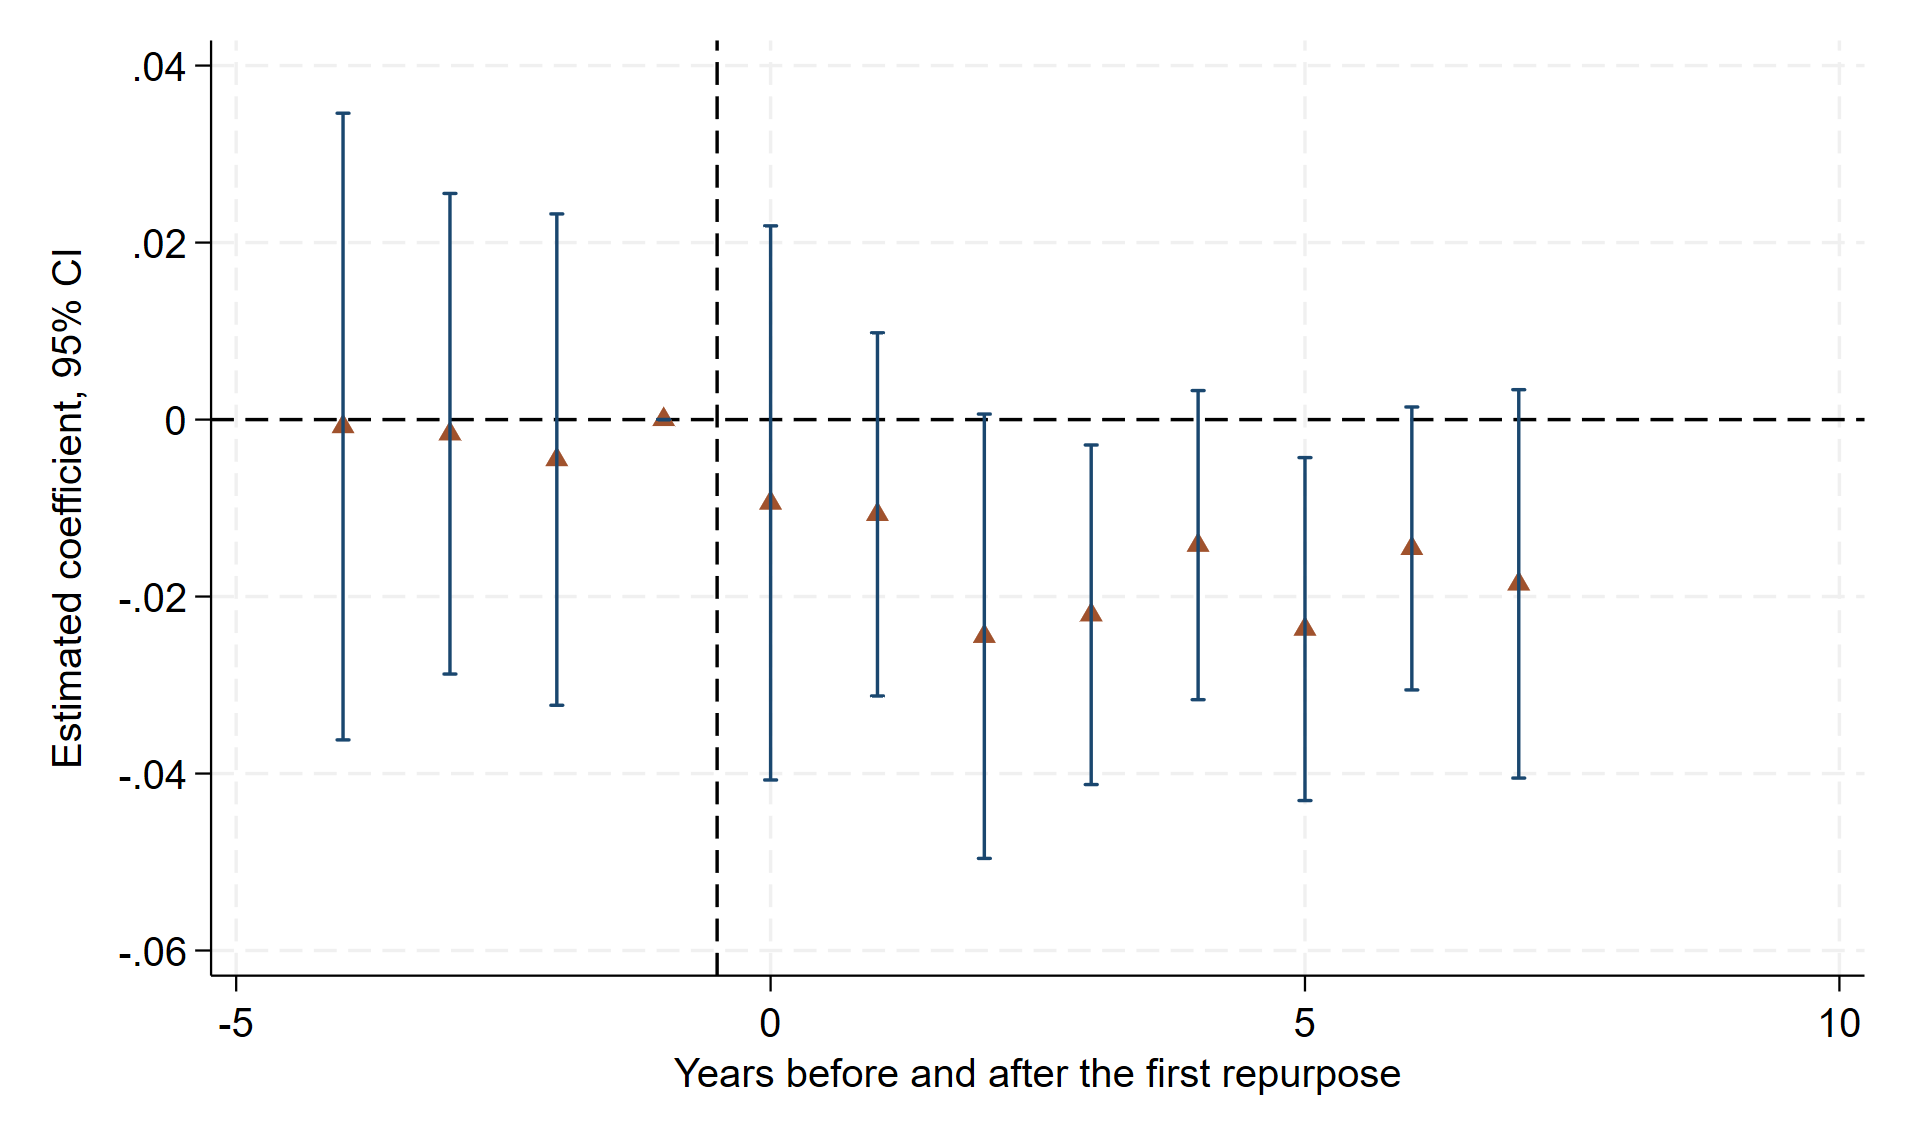
\includegraphics[scale=0.25]{pictures_1/mainevent_0826.png}
		\centering\caption{Estimated effects of the repurpose of Mafia properties on dropout rate before and after the first repurpose starts.}
		\label{fig:jmp_es_main}
	\end{center}
\end{figure}



Figure~\ref{fig:jmp_es_quality_het} presents the heterogeneous treatment effects across school catchment areas by baseline school quality. I construct a composite school quality indicator by first averaging standardized scores across academic outcomes and organizational and social processes, and then taking the row mean of these two sub-indices into an overall school performance measure. This index thus captures institutional effectiveness along both the outcome and process dimensions of school quality\footnote{Appendix~\ref{sec:jmp_app_D} discusses more in detail what the sub-indeces measures.}. Figure~\ref{fig:jmp_es_quality_het}a and~\ref{fig:jmp_es_quality_het}b report the treatment effects separately for schools below and above the median of the composite quality index. Both subsamples pass the parallel trends test, with F-test p-values of 0.143 and 0.941 respectively, lending credibility to the identifying assumption in each group. The effects are concentrated among low-performing schools, which exhibit larger point estimates and stronger statistical significance beginning two years after the first property reuse, while the estimates for high-performing schools remain small and imprecise. This heterogeneity suggests that the intervention operates through channels that are particularly effective in resource-constrained educational environments, where the marginal improvement in the surrounding social context translates into comparatively larger reductions in dropout rates. \par

    \begin{figure}[H]%
    \centering
    \subfloat[\centering Low Performing Schools]{{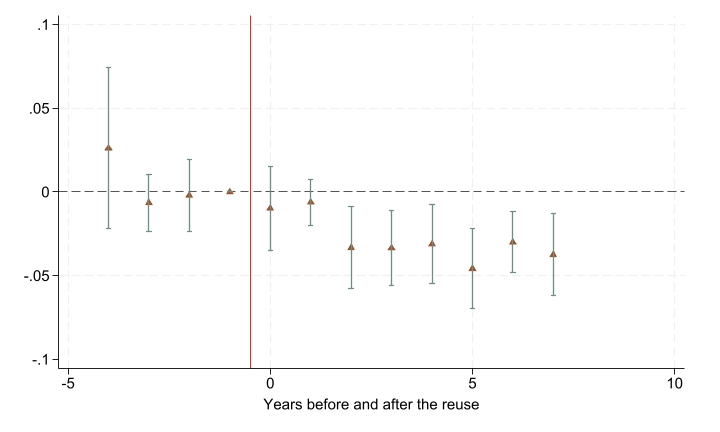
\includegraphics[width=7.4cm]{pictures_1/hetlowperf1.jpg} }}%
    \qquad
    \subfloat[\centering High Performing Schools]{{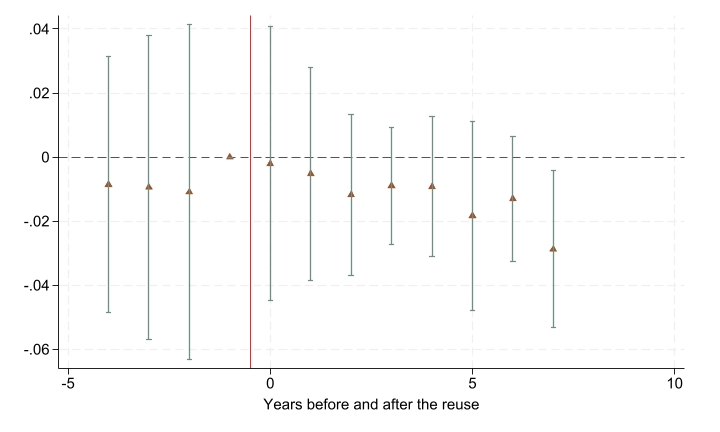
\includegraphics[width=7.4cm]{pictures_1/hetlowperf0.jpg} }}%
    \caption{Estimated effects of the repurpose of Mafia properties on dropout rates before and after the first repurpose starts by the baseline quality of schooling.
    }
    \label{fig:jmp_es_quality_het}

\end{figure}

I also explore heterogeneity by school track type. As explained in Section~\ref{sec:jmp_schools_data}, the Italian secondary educational system is divided in 14 specific high school sub-tracks, which can be grouped into three main tracks: academic, technical, and vocational high schools. I estimate three separate event studies to investigate whether the treatment effect shows different patterns for different tracks. The respective F-tests reveal p-values of 0.421, 0.651, and 0.333, confirming that I cannot reject the hypothesis that pre-treatment coefficients are jointly zero. \par
\medskip
The results reveal substantial heterogeneity across educational tracks in response to the repurpose intervention. Academic high schools, shown in Figure~\ref{fig:jmp_es_track_het}a, exhibit consistently small and statistically insignificant coefficients throughout the observation window, while vocational schools, shown in Figure~\ref{fig:jmp_es_track_het}c, display a similar  pattern, which is consistent with their institutional structure, whereby students obtain a professional qualification upon completing grade 11 rather than a full five-year diploma. Technical high schools, shown in Figure~\ref{fig:jmp_es_track_het}b, by contrast, show a more pronounced and sustained response, with negative effects on dropout rates that become statistically significant between two and four years after the first property repurpose.
This differential response likely reflects the distinct student populations and institutional contexts of each track. Technical schools occupy an intermediate position between academic preparation and vocational training, and their students appear particularly sensitive to the improved educational environment generated by the intervention. Research on the Italian education system documents that technical schools have experienced sharper declines in tertiary transition rates relative to other school types \citep{contini_too_2020}, suggesting these students face particular challenges in their educational trajectories. Unlike vocational students, who can enter the labour market with a three-year professional certificate, technical students require a full five-year diploma to meaningfully improve their employment prospects, making early dropout especially costly for this group. The improved educational incentives stemming from repurpose practices may therefore be especially valuable for students enrolled in technical programs.
Importantly, this pattern is not driven by compositional shifts in enrollment. Table~\ref{tab:jmp_enrollment_selection} shows that enrollment in technical schools does not change significantly following the treatment, indicating that the estimated effects operate through reduced dropout rather than student sorting across school tracks. \par

   \begin{figure}[H]%
    \centering
    \subfloat[\centering Academic High Schools]{{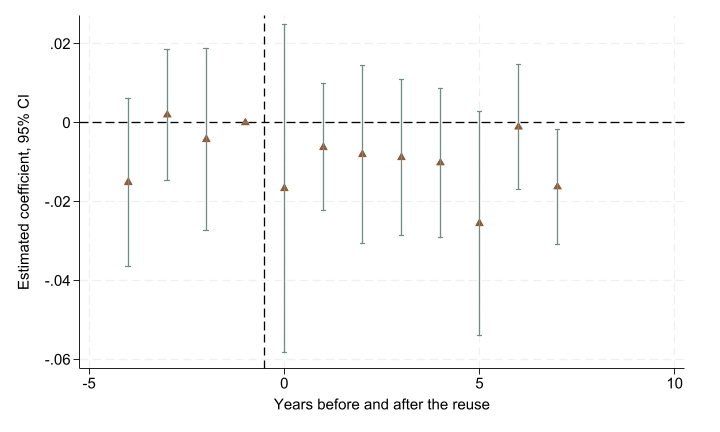
\includegraphics[width=7.4cm]{pictures_1/dummy_hetsch1.jpg} }}%
    \qquad
    \subfloat[\centering Technical High Schools]{{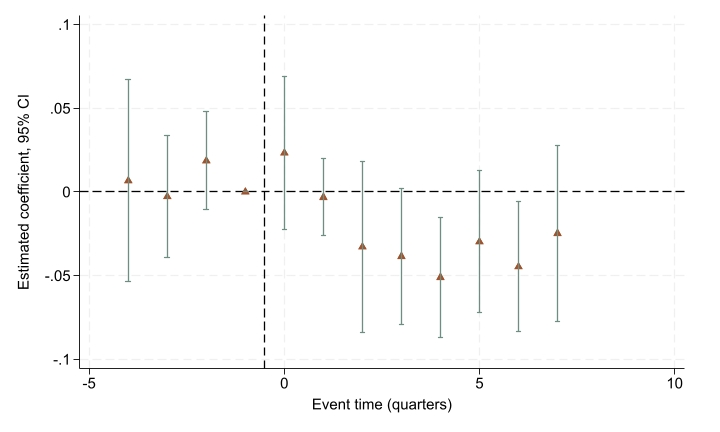
\includegraphics[width=7.4cm]{pictures_1/dummy_hetsch2.jpg} }}%
     \qquad
    \subfloat[\centering Vocational High Schools]{{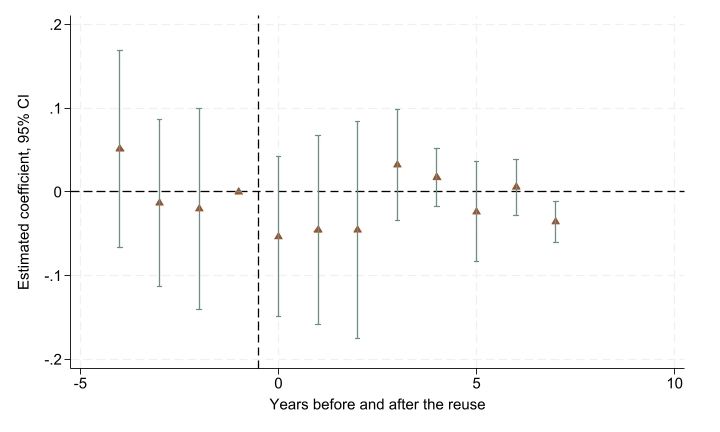
\includegraphics[width=7.4cm]{pictures_1/dummy_hetsch3.jpg} }}%
    \caption{Estimated effects of the repurpose of Mafia properties on dropout rates before and after the first repurpose starts by school track.
    }
    \label{fig:jmp_es_track_het}

\end{figure}

Beyond school characteristics, the treatment effect may also vary heterogeneously with the characteristics of the repurposed Mafia properties. 

I start analysing the heterogeneity of the ATE based on the basic attributes of repurposed properties. Following \citet{operti_tough_2018}, I define \emph{operational properties} all those residential real estate which belonged to the Mafia family signaling their local sovereignity,  and \emph{economic properties}, such as real estate units used for commercial purposes. Figure~\ref{fig:jmp_es_property_het} reveals that the effect is driven by school catchment areas treated by the presence of at least one operational property, while those treated by economic properties alone show no statistically significant effect. The results are further concentrated among independent residential units and agricultural land, rather than industrial deposits or garages. \par

\begin{figure}[H]%
	\centering
	\subfloat[\centering Property use before confiscation]{{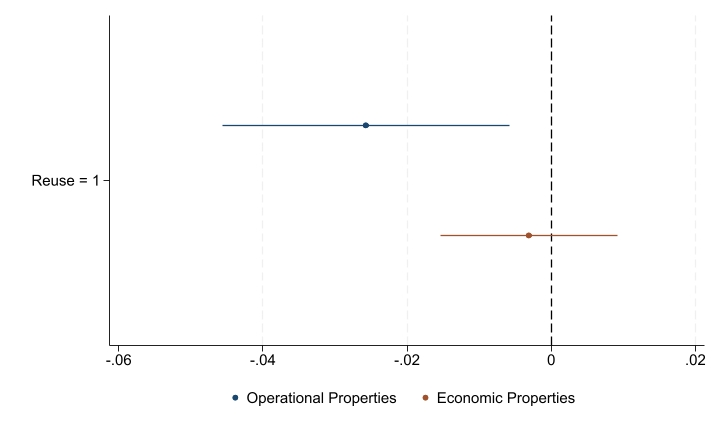
\includegraphics[width=7.4cm]{pictures_1/het_operational_econ.jpg} }}%
	\qquad
	\subfloat[\centering Property type]{{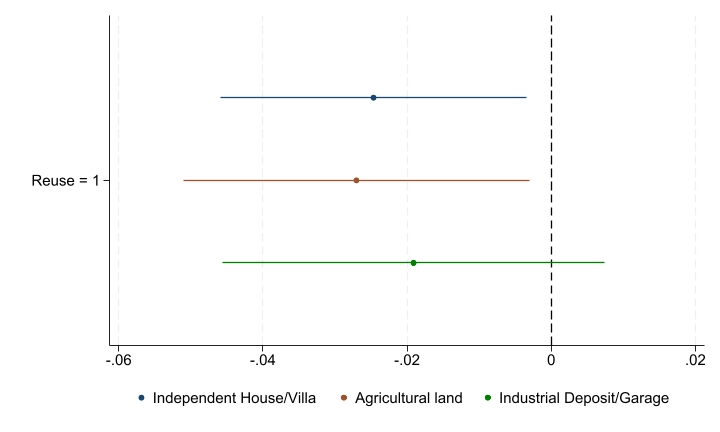
\includegraphics[width=7.4cm]{pictures_1/het_typeofasset.jpg} }}%
	\caption{Estimated effects of the repurpose of Mafia properties on dropout rates before and after the first reuse starts by properties' features.
	}
	\label{fig:jmp_es_property_het}
	
\end{figure}

Second, I investigate whether the effects are driven by the specific type of activity hosted in the repurposed property. If the intervention worked by adding educational and training resources, properties dedicated to education and employment should generate larger effects than those used for cultural or welfare purposes. To test this, I decompose the treatment effect by activity type. Since categories are not mutually exclusive as a catchment area may contain properties offering several types of activity, I estimate separate specifications for each category. In each regression, I compare treated areas where at least one property offers activities of a given type to never- and not-yet-treated areas, while controlling for treated areas whose properties offer no activity of such nature. I describe the specification in Appendix~\ref{sec:jmp_app_D} and report the coefficients in Figure~\ref{fig:jmp_cats_repurpose}.
The main feature of the decomposition is how little the point estimates differ across categories. All four lie between a decrease of 1.5 and 1.8 percentage points in the level of dropout rate, corresponding to reductions of roughly 28 to 33 per cent relative to the baseline mean. What we can distinguish is precision rather than magnitude: cultural activities yield a confidence interval lying entirely below zero, welfare activities are significant at the 90 per cent level, while education and employment activities carry intervals that comfortably cross zero.\footnote{Regression results are reported in Table~\ref{tab:jmp_repurpose_types}.} The wider intervals for the latter two reflect the smaller number of catchment areas hosting such activities rather than a weaker underlying effect.

This pattern is informative in a different way than a concentration result would be. Had the effect been driven by educational provision, properties delivering education and employment services should have produced systematically larger estimates than those hosting cultural or welfare activities. They do not. The dropout reduction appears to be broadly invariant to what the repurposed property is used for, which is difficult to reconcile with a mechanism operating through the content of the activities themselves and points instead toward a channel that depends on the visible reclaiming of the property rather than on the services delivered within it. \\

\begin{figure}[H]%
	\centering
	{{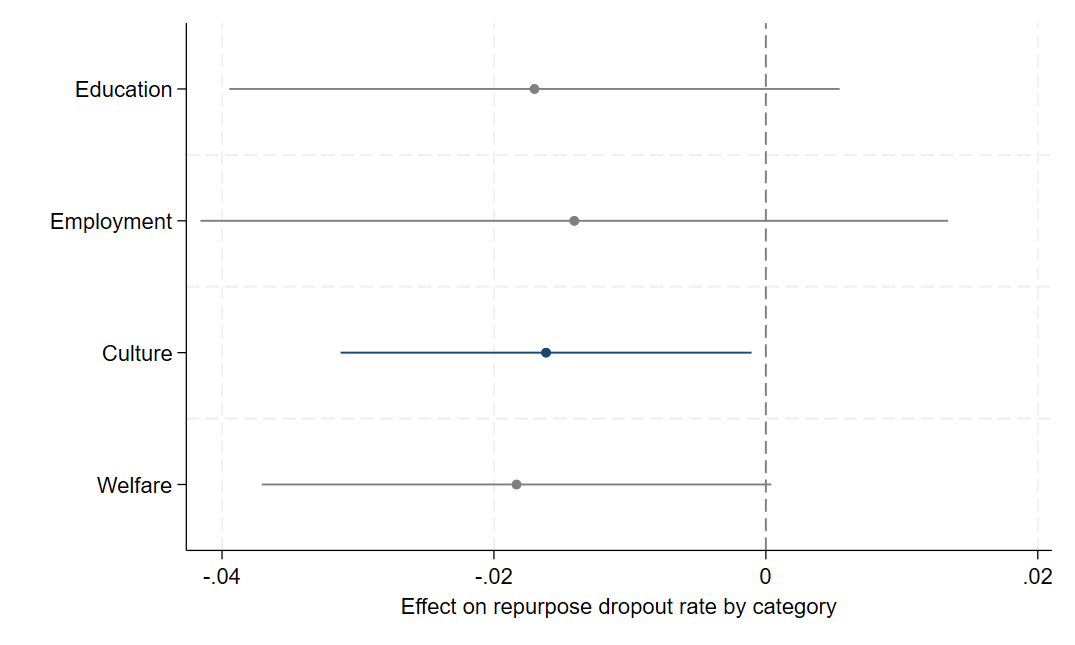
\includegraphics[width=15.4cm]{pictures_1/cats_rep.png} }}%
	\caption{Estimated effects of the repurpose of Mafia properties on dropout rates before and after the first reuse starts by type of activity in the repurposed property.
	}
	\label{fig:jmp_cats_repurpose}
	%say that the new policy gave a new emotional wave on the reallocation in general
	
\end{figure}

Last, the treatment effect may also vary with the number of confiscated properties repurposed within a given catchment area and their spatial distribution relative to the student population. I therefore examine whether the estimated effects are driven solely by the first reuse event or whether they intensify with cumulative exposure to multiple repurposed properties over time. The underlying hypothesis is that the impact of reuse practices on student outcomes need not materialise immediately upon first treatment, but may instead unfold gradually, shaped by both the timing of individual reuse events and the accumulating density of repurposed properties within the catchment area. In particular, treatment effects are expected to grow stronger as the stock of reused properties increases and as their locations overlap more closely with where students actually reside. To investigate this, I split the sample into schools whose catchment area experienced at most one repurpose event over the entire observation period and those exposed to multiple repurpose practices. Table~\ref{tab:jmp_intensity} reports the results, revealing a potential dose-response relationship between reusing practices and dropout reduction. Columns (1) and (2) show that schools whose catchment areas experienced only a single reuse event exhibit small and statistically insignificant effects on dropout rates. By contrast, schools exposed to multiple repurposed properties, which are reported in Columns (3) and (4), display substantially larger and precisely estimated reductions, corresponding to declines of 51\% and 48\% relative to the mean, respectively. This pattern suggests that cumulative exposure to repurpose practices amplifies the treatment effect, pointing to a dose-response relationship whereby the educational benefits of the treatment intensify as the number of repurposed properties within the catchment area grows.  \par
\medskip


\begin{table}[H]
\caption{Impact of repurposing Mafia real estate on the share of students dropping out from grades 11 to 13 by intensity of exposure.} % Table label
\label{tab:jmp_intensity}
\vspace{0.2cm}
\centering
\scalebox{0.8}{
          \begin{tabular}{p{9.355em}llll}
    \toprule
    \multicolumn{1}{l}{} & \multicolumn{1}{c}{(1)} & \multicolumn{1}{c}{(2)} & \multicolumn{1}{c}{(3)} & \multicolumn{1}{c}{(4)} \\
    \multicolumn{1}{l}{Dep: Dropout 3-5 years} & \multicolumn{2}{c}{\textbf{Properties reused = 1}} & \multicolumn{2}{c}{\textbf{Properties reused $>$ 1}} \\
    \midrule
    \multicolumn{1}{l}{} & \multicolumn{1}{c}{} & \multicolumn{1}{c}{} & \multicolumn{1}{c}{} & \multicolumn{1}{c}{} \\
    \multicolumn{1}{l}{Reuse = 1} & \multicolumn{1}{c}{-0.00284} & \multicolumn{1}{c}{-0.00466} & \multicolumn{1}{c}{-0.0293**} & \multicolumn{1}{c}{-0.0277**} \\
    \multicolumn{1}{l}{} & \multicolumn{1}{c}{(0.0133)} & \multicolumn{1}{c}{(0.0139)} & \multicolumn{1}{c}{(0.0123)} & \multicolumn{1}{c}{(0.0119)} \\
    \multicolumn{1}{l}{} & \multicolumn{1}{c}{} & \multicolumn{1}{c}{} & \multicolumn{1}{c}{} & \multicolumn{1}{c}{} \\
    \multicolumn{1}{l}{Observations} & \multicolumn{1}{c}{541} & \multicolumn{1}{c}{522} & \multicolumn{1}{c}{755} & \multicolumn{1}{c}{750} \\
    \multicolumn{1}{l}{Number of codd} & \multicolumn{1}{c}{101} & \multicolumn{1}{c}{101} & \multicolumn{1}{c}{134} & \multicolumn{1}{c}{133} \\
    \multicolumn{1}{l}{clustered SE} & \multicolumn{1}{c}{yes} & \multicolumn{1}{c}{yes} & \multicolumn{1}{c}{yes} & \multicolumn{1}{c}{yes} \\
    \multicolumn{1}{l}{school FE} & \multicolumn{1}{c}{yes} & \multicolumn{1}{c}{yes} & \multicolumn{1}{c}{yes} & \multicolumn{1}{c}{yes} \\
    \multicolumn{1}{l}{time FE} & \multicolumn{1}{c}{yes} & \multicolumn{1}{c}{yes} & \multicolumn{1}{c}{yes} & \multicolumn{1}{c}{yes} \\
    \multicolumn{1}{l}{migration} & \multicolumn{1}{c}{no} & \multicolumn{1}{c}{yes} & \multicolumn{1}{c}{no} & \multicolumn{1}{c}{yes} \\
    \multicolumn{1}{l}{retention} & \multicolumn{1}{c}{no} & \multicolumn{1}{c}{yes} & \multicolumn{1}{c}{no} & \multicolumn{1}{c}{yes} \\
    \multicolumn{1}{l}{Observations} & \multicolumn{1}{c}{541} & \multicolumn{1}{c}{522} & \multicolumn{1}{c}{755} & \multicolumn{1}{c}{750} \\
    \multicolumn{1}{l}{Number of schools} & \multicolumn{1}{c}{101} & \multicolumn{1}{c}{101} & \multicolumn{1}{c}{134} & \multicolumn{1}{c}{133} \\
    \multicolumn{1}{l}{Mean dep. var.} & \multicolumn{1}{c}{0.0485} & \multicolumn{1}{c}{0.0477} & \multicolumn{1}{c}{0.0574} & \multicolumn{1}{c}{0.0568} \\
    \midrule
    \multicolumn{5}{p{35.935em}}{Notes: TWFE model. The treatment variable is equal to 1 whenever there is at least one reused Mafia property within the school catchment area. Columns (1) and (3) do not include controls while Columns (2) and (4) include them. Standard errors are clustered at the school level.} \\
    \end{tabular}%
    }
\end{table}

I take a step forward and I directly estimate the dynamic evolution of the treatment effect generated by the repurpose of confiscated Mafia properties. I perform three subsequent exercises: first, I estimate a dynamic DiD model using an event study approach. This framework allows me to follow the evolution of the treatment effect relative to the timing of the repurpose and to assess whether the observed impacts arise from a gradual buildup of exposure to reusing activities. I employ the estimator proposed by \citet{de_chaisemartin_difference--differences_2024}, which computes the cumulative effect of each treatment dose across all time periods and determines how long these effects persist on average. 
Figure~\ref{fig:jmp_es_continuous} displays the event study of the dynamic evolution of the treatment effect. The control and treated groups do not appear to exhibit differential pre-trends, as indicated by the F-test on the pre-treatment coefficients with a p-value of 0.330.
Figure~\ref{fig:jmp_es_continuous} displays the average cumulative treatment effect per additional reused property on dropout rates, where each coefficient captures the total impact of one further reuse event accumulated over all subsequent periods. The overall average effect is negative and equal to 0.64 percentage points, implying that each additional repurposed property reduces dropout rates by approximately 12\% relative to the mean. Importantly, the magnitude of this effect varies considerably with the timing of reuse: properties repurposed in the first and second year of treatment are associated with reductions of 0.04 and 1.9 percentage points respectively, whereas those reused four and five years after the initial treatment generate substantially larger reductions of 3.8 and 5.2 percentage points. This monotonically increasing pattern suggests that the educational returns to property reuse compound over time, with sustained, long-term programs hosted in repurposed Mafia assets generating substantially greater benefits than early or isolated activities. \\

\begin{figure}[H]
  \begin{center}
    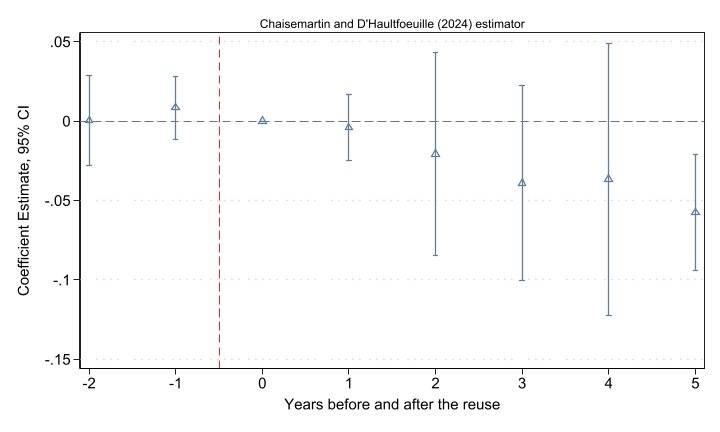
\includegraphics[scale=0.75]{pictures_1/cont_baseline.jpg}
    \centering\caption{Average cumulative treatment effect of repurposing Mafia real estate on dropout rates, by repurpose intensity and timing.}
    \label{fig:jmp_es_continuous}
    \end{center}
    \end{figure}

 I next re-estimate the event study by weighting the count of reused assets by the student population within each school catchment area. While the count-based measure captures the overall intensity of repurpose activities, it does not account for the size of the student population that could potentially benefit from them. 
The results, reported in Appendix~\ref{sec:jmp_app_A}, closely mirror those obtained under the simple count specification and are if anything stronger. Figure~\ref{fig:jmp_es_stw} shows a reduction of 4.5 percentage points in dropout rates, suggesting that treatment intensity matters: repurpose activities generate larger educational returns when concentrated relative to the local student population rather than dispersed across larger catchment areas.
I further validate these findings through a distance-weighted specification, in which the treatment measure is weighted by the average distance of repurposed properties from the population-weighted centroid of each catchment area. Figure~\ref{fig:jmp_es_dist} confirms the previous results, yielding an estimated reduction in dropout rates of 5 percentage points. Taken together, both alternative specifications reinforce the conclusion that the spatial concentration of repurpose activities relative to the student population is a meaningful determinant of treatment effectiveness. \par

    
%%%%%%%%%%%%%%%%%%%%%%%%%%%%%%%%%%%%%%%%%%%%%%%%%%%%%%%%%%%%%%%%%%
\FloatBarrier
\section{Effects on Students' Beliefs}
\label{sec:jmp_mechanisms}

Repurposing Mafia properties for social use decreases the levels of dropout rate for schools located nearby. These effects are particularly pronounced for technical high schools and lower-performing schools. The main decrease is driven by the repurpose of properties that were previously used as luxurious Villas and apartments formerly owned by Mafia families, while prior to repurpose we do not find any significant effect of confiscations and reallocations on educational outcomes.  Notably, the reduction is concentrated in properties hosting cultural activities, rather than those providing direct educational or vocational resources, pointing to a community-level rather than a purely educational-input channel. Moreover, a dose-response pattern emerges, with each additional repurposed property amplifying the reduction in dropouts.  In this Section I investigate the mechanisms behind the estimated effects presenting both empirical and anecdotical evidence; the results suggest that the decrease in dropout is driven by a change in students' beliefs about the importance of meritocratic channels for job-seeking, as well as the reasons why people should turn to the Mafia. Additionally, I find that students believe the Mafia is a weaker force, while they perceive an increase in their own empowerment as civil society and the State's capacity to face the Mafia. Last, I don't observe significant changes in the local opportunity structure which might drive the effects, such as Mafia recruitment levels, additional educational support delivered in repurposed properties, and a concurrent ongoing gentrification process.\par
\medskip

\subsection{Students' Aspirations}
\label{sec:jmp_perception}
The central aim of repurposing former Mafia-owned properties is to change the local opportunity structure local residents face, both considering what they experience and what they perceive of their surrounding reality. Acknowledging that arresting Mafia groups is only the first enforcement step of the policy, the State seeks to send a strong message by building capacity in these infiltrated areas, replacing criminal governance with visible institutions that serve the community. According to this, there are two main mechanisms that could be driving the effect: a change in the way juveniles perceive their future options, and a change in what their options are. On the one hand, it could be the case that after seeing a physical change and after getting aware about the socio-economic effect of the Mafia, juveniles change their perspective about Mafia's reputation and social status and they might prefer to follow meritocratic channels for job-seeking and career advancement. This would reduce the perceived benefits of joining the Mafia, while push juveniles to substitute for alternative job-seeking channel. On the other hand, the results could be driven by an increase in the educational support provided to juveniles on these properties, such as after-school programmes and educational mentoring activities which account for around the 10\% of the existing activities carried out. This way, once facilitated in their educational journey, juveniles will face a lower cost of staying in education. \\

Recent conversations with \emph{Libera}'s repurpose team managers and social workers from the NGOs working in the repurposed properties, together with the interviews conducted by \citet{nazzaro_il_2021} and \citet{falcone_beneitalia_2016}, lend support to the idea that these interventions reshape local attitudes toward the Mafia. NGOs' workers describe these places as gathering centres for the local community, attracting people of all ages to take part and put efforts into transforming the previously infiltrated area; renovating social bonds and reclaiming the local area through the participatory redevelopment of these properties seems to address a local change of perspective. \\
Interviews conducted by \citet{nazzaro_il_2021} highlight that \par

\vspace{0.5cm}
\footnotesize{
	Directly involving citizens in various activities for the redevelopment of former Mafia properties is important in the perception of that space as a newly acquired common space that had previously been taken away for criminal purposes. 
	- Interview from the NGO \emph{AGESCI}, Apulia, Italy} \par
\vspace{0.5cm}

\normalsize
Moreover, especially considering the juveniles' experiences, \citet{nazzaro_il_2021} reports that \par

\vspace{0.5cm}
\footnotesize"On properties and lands confiscated from the Mafia [...] we find experiences featuring many young people, who were the first to decide to participate, aware of the importance of what was at stake."  - \emph{Carlo Borgomei, President of Fondazione Con il Sud}
\vspace{0.6cm}

\normalsize
On the same topic, \citet{falcone_beneitalia_2016} reports that \par

\vspace{0.5cm}
\footnotesize{
	This policy has served to develop NGOs gathering juveniles who work in the sector of sustainable agriculture and develop new markets that did not exist until the day before, and has introduced and consolidated in our society a strong and open message: it is indeed possible to build a different future, where many and many different people in terms of culture, profession and age participate to make it happen. - \emph{Lucio Cavazzoni, president of Alce Nero,} interview from Libera} \par
	\vspace{0.5cm}
	\normalsize 		

	To provide more nuanced empirical evidence, I examine how these interventions alter students' perceptions about educational and criminal pathways to career development in their communities. I employ TWFE models using data from the survey \emph{The Perception of the Mafia}, which was collected from a subsample of schools. The survey covers 54 schools with an average of 110 students per school. Out of the total sample, 24 schools are treated while 30 serve as controls.
	I first exploit the answers given to the question: \emph{What of this options you think will be more useful for you to find a job in your town?}. Students were asked to rate several job-seeking channels on a scale from 1 - as the most useful - to 7 as the most useless. The options include several meritocratic channels, such as embark in an educational training, refer to a job centre, take a competitive examination for civil service, and several informal channels such as asking the Mafia, a politician, family, or a friend. If the repurpose of Mafia properties reduces the attractiveness of criminal pathways and the expected returns of joining the Mafia, students in treated areas should place greater value on other employment channels, whether formal or informal, depending on whether they substitute toward legal or illegal alternatives.
	Figure~\ref{fig:jmp_survey_career} presents the ATT estimated under a DiD design that includes school fixed effects and time fixed effects\footnote{Regressions table results are reported in Table~\ref{tab:jmp_v28}}; I also weight each school by the number of students replying to the survey to account for varying school sizes in the survey sample. The outcome variables represent the percentage of students for each school who rated each pathway as a \emph{very useless}  or \emph{very useful} option, allowing me to identify whether repurposed Mafia properties systematically alter the distribution of student perceptions within schools. Following previous literature \citep{villa_effect_2025}, I focus on the extreme categories of student responses to better capture meaningful shifts in perceptions\footnote{I measure the most useful choices as the percentage of students that rate each option with 1 or 2, and the most useless choices as the percentage of students that rate each option with 6 ot 7.} Finally, standard errors are clustered at the school level across all specifications. \\
	The results reveal compelling evidence of altered student perceptions consistent with a weakened criminal influence and a strengthened belief in legitimate pathways. 
		The left panel (a) examines the effect of reusing activities on the probability of rating each pathway as \emph{very useful}. Most notably, students in areas with repurposed Mafia properties are significantly more likely to view education training as very useful, with a substantial 34\% increase relative to the baseline, indicating that the intervention meaningfully enhances students' perception of education as a pathway to employment success. A similar pattern emerges for how students perceive civil-service examinations: students in treated areas are more likely to rate this channel as very useful, a reduction of roughly 84\% relative to the baseline mean of 0.163, though the effect is only marginally significant (t = 1.65).	The right panel (b) examines the effect of reusing activities on the probability of rating each pathway as \emph{very useless}. Most notably, students in areas with repurposed Mafia properties are 24\% more likely to rate the option to ask for help from the Mafia as very useless, while they are 26\% more likely to rate the option to ask a politician for help as very useless. Overall the results suggest that students come to view Mafia connections as a weaker and less useful route to employment, the expected benefit of that pathway falls, reducing the incentive to leave school early to pursue it. The observed reduction in dropout rates is therefore consistent with a mechanism that works chiefly by eroding the attractiveness of the criminal channel, with the strengthened perception of education as a legitimate alternative reinforcing, rather than driving, the effect.
	
	\begin{figure}[H]%
		\centering
		{{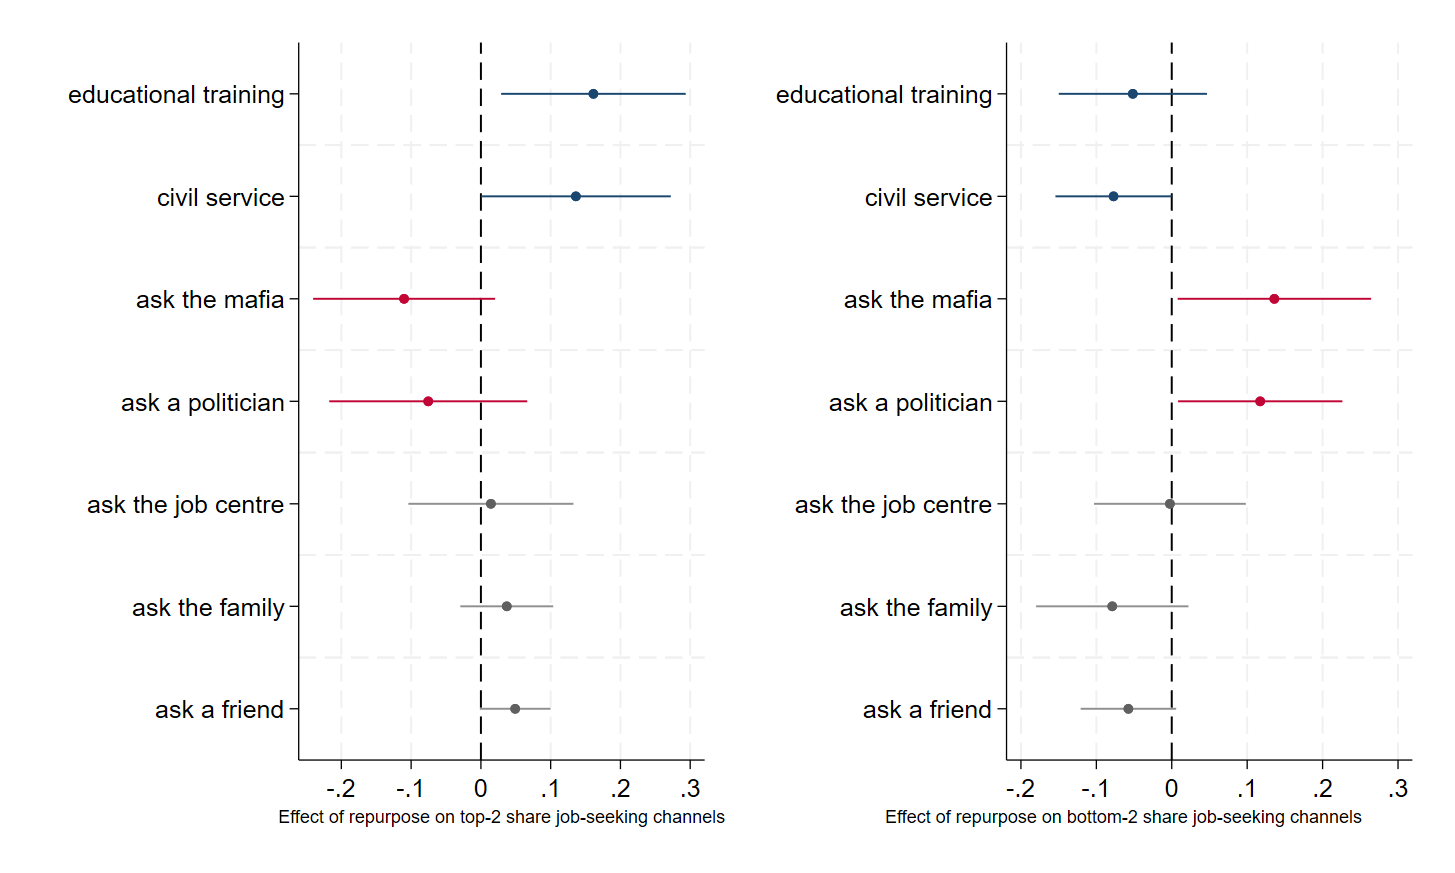
\includegraphics[width=15.4cm]{pictures_1/v28_coeffplot.png} }}%
		\caption{Estimated effects of repurposing practices on students' survey answers about career development. The left panel (a) reports the effect of reuse on the share of students ranking each channel among the two \emph{most} important routes to career success; the right panel (b) reports the effect on the share ranking each channel among the two \emph{least} important. Coefficients are from separate regressions with school and year fixed effects, weighted by the number of students and with standard errors clustered at the school level; results are significant at the 90\% confidence level.
		}
		\label{fig:jmp_survey_career}
		%say that the new policy gave a new emotional wave on the reallocation in general
		
	\end{figure}
	

		\begin{figure}[H]%
		\centering
		{{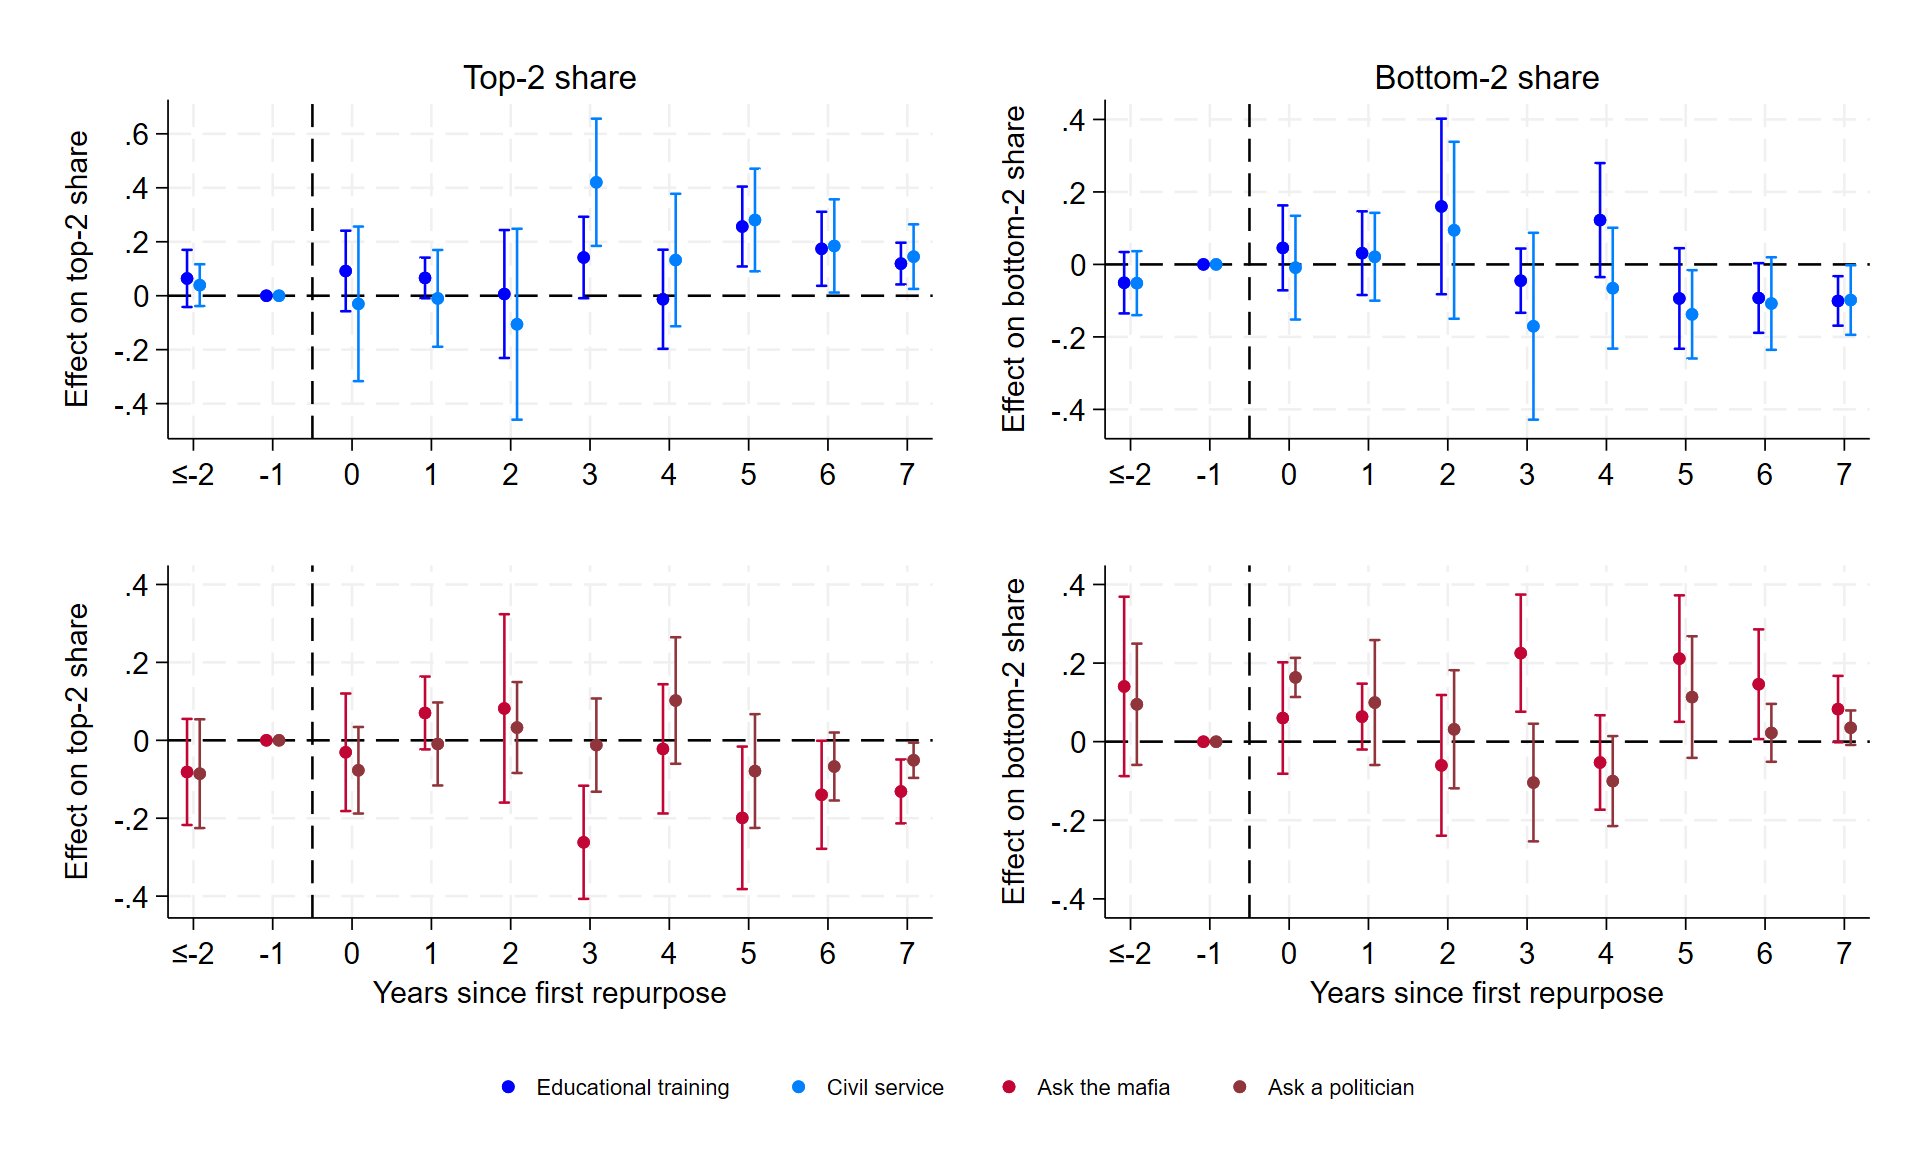
\includegraphics[width=15.4cm]{pictures_1/beliefs_eventstudy.png} }}%
		\caption{Event studies of repurposing practices on students' survey answers about career development. The left panels report the effect of repurpose on the share of students ranking each channel among the two \emph{most} important routes to career success; the right panels report the effect on the share ranking each channel among the two \emph{least} important. Coefficients are from separate regressions with school and year fixed effects, weighted by the number of students and with standard errors clustered at the school level; results are significant at the 90\% confidence level.
		}
		\label{fig:jmp_event_beliefs}
		%say that the new policy gave a new emotional wave on the reallocation in general
		
	\end{figure}
	The event study estimates in Figure~\ref{fig:jmp_event_beliefs} speak directly to the timing of the mechanism. Across the four channels, the pre-treatment coefficients are flat and statistically indistinguishable from zero\footnote{Due to a small sample, I am unable to retrieve more information about pre-trends.}, supporting the parallel-trends assumption underlying the design. The post-treatment movements are concentrated in the two channels most central to the mechanism and emerge on a common horizon: the share of students ranking the Mafia among the most useful employment routes falls, and its share among the least useful rises, while the standing of the civil-service examination among the most useful routes. Both effects materialise around the third year fo treatment, moving over the same period. The remaining channels move less precisely, consistent with the intervention acting chiefly on the perceived returns to the criminal pathway and its most direct meritocratic substitutes.
	
	This timing is informative for the concern that a change in perceptions should either precede or coincide with a behavioural change. The belief shift materialises only from the second-to-third year after repurpose, and it does so on the same horizon at which the reduction in dropout becomes statistically significant in Figure~\ref{fig:jmp_es_main}. The co-timing of the two responses is what the proposed mechanism predicts. Repurposing does not change the local opportunity structure overnight: the property must be assigned, an NGO must take it over, and its activities must become an established and visible presence in the community before residents' assessment of the relative attractiveness of criminal and legal pathways begins to shift. The delay of roughly three years is therefore not evidence against the mechanism but a signature of it, as a gradual erosion of the perceived returns to the Mafia channel, reflecting in students' stated beliefs and in their enrolment decisions at the same time.
	
	
	%I next examine how the intervention reshapes students' understanding of \emph{why} people turn to the Mafia in the first place, drawing on a survey question that asks respondents to identify the main reason for joining the Mafia. In this case, students are given a multiple choice question. Figure~\ref{fig:jmp_survey_career2} reports the estimated effects, while regression tables are reported in Table~\ref{tab:jmp_v30}. Students in treated areas are markedly more likely to attribute Mafia membership to family ties and to the desire to make easy money, with increases of respectively 62\% and 41\% relative to their baseline means. At the same time, they are considerably less likely to explain Mafia affiliation as a response to the search for employment, a decline of about 63\% relative to the baseline mean. The remaining categories show no significant change. Taken together, these results suggest that the intervention erodes the perception of the Mafia as a legitimate response to economic necessity, shifting students toward an interpretation grounded in cultural ties and the desire for illicit gain. \\
	
		%	\begin{figure}[H]%
			%\centering
		%	{{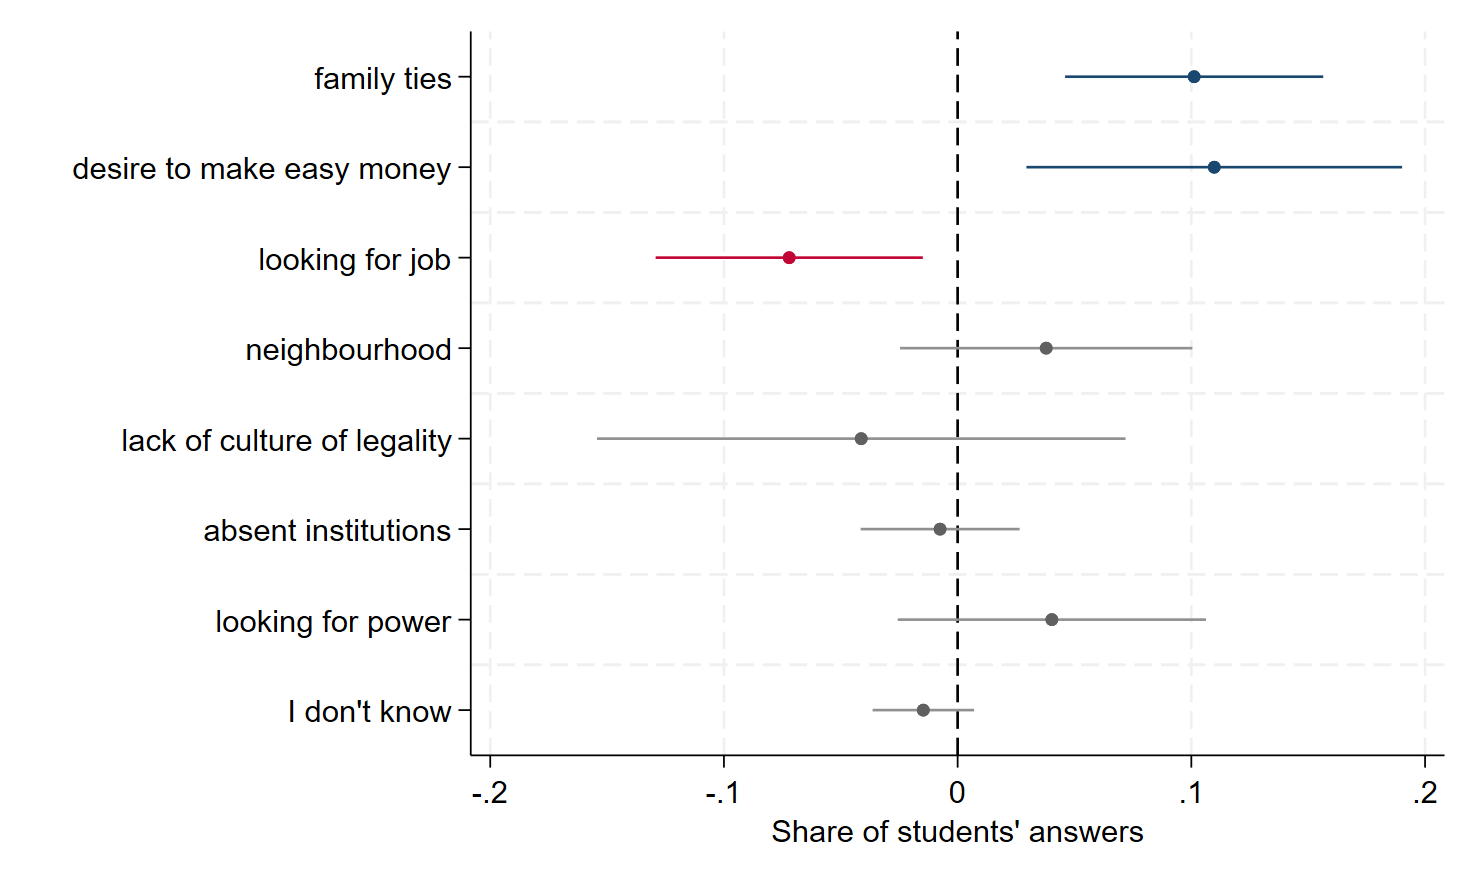
\includegraphics[width=15.4cm]{pictures_1/v30_coeffplot.png} }}%
		%	\caption{Estimated effects of reusing practices on students' stated reasons for why people join the Mafia. Each point reports the effect of reuse on the share of students selecting a given reason, estimated from separate regressions that include school, year, and grade fixed effects, are weighted by the number of students, and cluster standard errors at the school level. Navy markers denote the two reasons framing Mafia membership as rooted in family ties and the desire for easy money; the cranberry marker denotes the economic-necessity reason (looking for a job). Results are significant at the 95\% confidence level.}
	
		%	\label{fig:jmp_survey_career2}
		%say that the new policy gave a new emotional wave on the reallocation in general
		
	%	\end{figure}
	
	

	
	\FloatBarrier
	\subsection{Trust in State Capacity}
The evidence so far suggests that repurposing properties reduces the level of dropout by shifting how students evaluate criminal versus legal pathways to career advancement. It is possible that the interventions raise the expected returns from education by strengthening students' belief that education leads to legitimate employment, and it could lower the expected return to a criminal career, as students come to see Mafia connections as a weaker and less rewarding route to advancement. However, it is also possible that the repurpose of Mafia properties raise the perceived cost of joining the Mafia as the visible reclaiming of a property signals a more present and capable State and thus a higher perceived probability of enforcement. These interpretations are not mutually exclusive, but distinguishing between them clarifies what the policy actually changes. \\

Two further survey questions let me examine whether repurposing shifts students' perceptions of the State's capacity. The first asks the students' level of agreement with a series of statements about the relative strength of the State and the Mafia. The second asks the students to rate the most and least trusted institutional actors among several choices, allowing me to measure whether the intervention raises confidence in the formal institutions that embody State capacity. Figure ~\ref{fig:jmp_trust1} shows that students' are less likely to agree with the fact that the Mafia is stronger because it infiltrates the State, and that the State does too little to fight the Mafia, respectively by 4.3\% and 24\% relative to the mean. I further test the dynamics effects of repurpose on these two perception measures. The estimates are imprecise and most individual coefficients cannot be distinguished from zero. The point estimates are nonetheless suggestive: for both measures coefficients  turn negative in the first years after repurpose before returning toward zero at longer horizons, consistent with a shift toward greater confidence in State capacity. While we interpret these results cautiously given the absence of estimable pre-treatment coefficients, the pattern is consistent with the static estimates. Notably, the shift in perceived State capacity appears earlier than the other mechanism responses: it emerges in the first years after repurpose, whereas the change in students' preference of employment channels and the reduction in dropout become pronounced only from around the third year. This ordering is consistent with the proposed mechanism, in which the visible reclaiming of the property first alters students' perception of the State's presence and capacity, and the shift in students' beliefs about legal and illegal pathways follows as that perception takes hold. I therefore read these dynamics as corroborating the estimates from Figure~\ref{fig:jmp_trust1}, and as suggestive that the State-capacity channel might operate upstream of the other responses.

		\begin{figure}[H]%
	\centering
	{{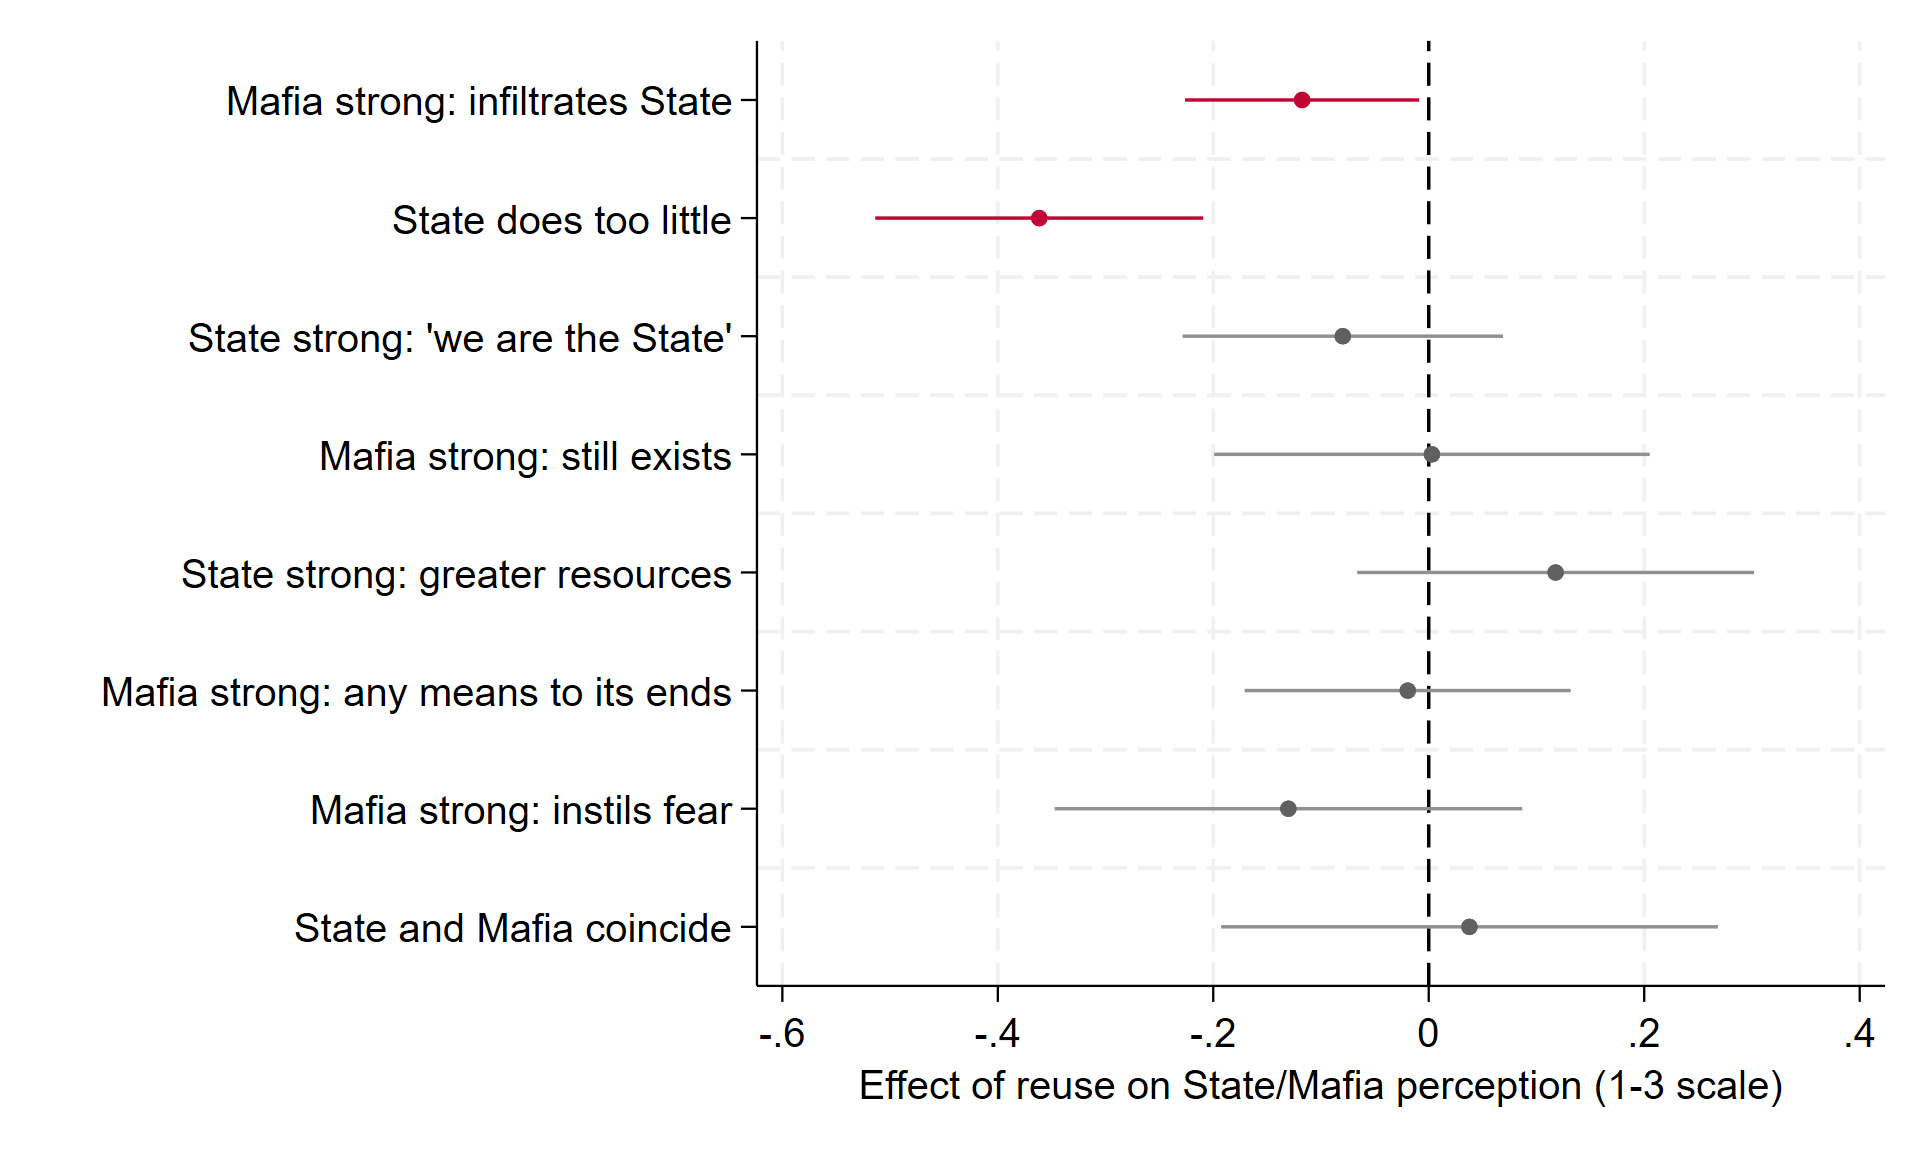
\includegraphics[width=11.4cm]{pictures_1/v30_new_0826.png} }}%
	\caption{Estimated effects of repurposing practices on students' agreement with statements about the strength of the Mafia and the State. Each point reports the effect of repurpose on the share of students rank of statements, estimated from separate regressions that include school and year fixed effects, and are weighted by the number of students. Standard errors are clustered at the school level. Results are significant at the 90\% confidence level.}
	
	\label{fig:jmp_trust1}
	%say that the new policy gave a new emotional wave on the reallocation in general
	
\end{figure}



		\begin{figure}[H]%
	\centering
	{{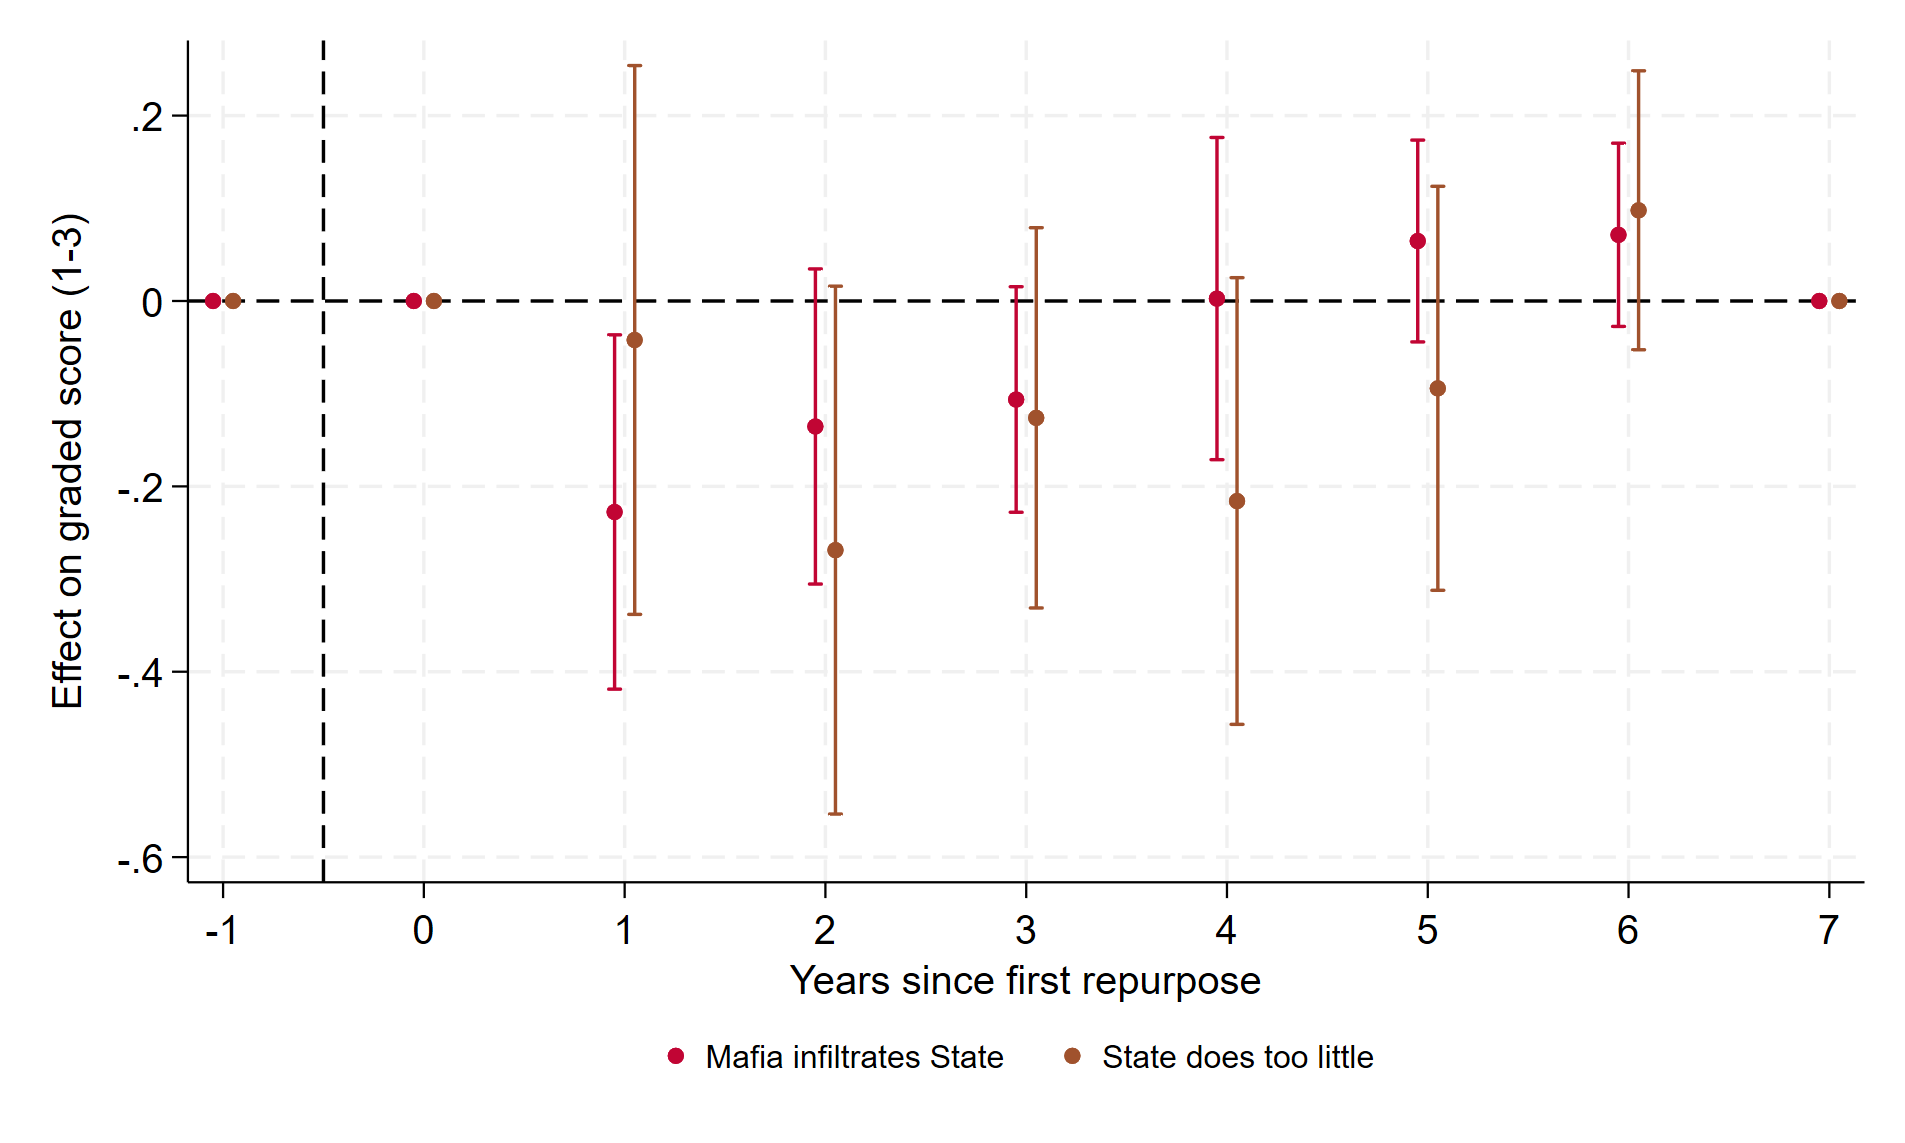
\includegraphics[width=10.4cm]{pictures_1/event_trust.png} }}%
	\caption{Event studies of repurposing practices on students' agreement with statements about the strength of the Mafia and the State. Each point reports the effect of repurpose on the share of students rank of statements, estimated from separate regressions that include school and year fixed effects, and are weighted by the number of students. Standard errors are clustered at the school level. Results are significant at the 90\% confidence level.}
	
	\label{fig:jmp_trust1_ev}
	%say that the new policy gave a new emotional wave on the reallocation in general
	
\end{figure}

	If repurposing strengthens perceived State capacity and raises the perceived cost of joining the Mafia, we should also observe changes in how much students trust the institutional bodies that represent the State. Figure~\ref{fig:jmp_trust2} reports the effect of reuse on the share of students naming each institution as their most and least trusted. The effects are concentrated on the least-trusted margin and among the institutions most directly associated with the State's local enforcement and governance. Students in treated areas are significantly less likely to name the police and local politicians among the institutions they trust least — by 30\% and 42\% relative to the mean, respectively. As the most-trusted margin shows no comparable shift, the intervention appears to work by eroding active distrust of core State institutions rather than by generating enthusiasm for them: a more modest but arguably more plausible change, since reclaiming a single property is more likely to soften scepticism about the State's presence than to produce positive endorsement of it.

This reading fits the state-capacity channel. Police and local politicians are precisely the actors whose credibility is undermined where the Mafia governs in the State's place; a fall in distrust for police and local politicians is consistent with students perceiving the State as a more present and capable authority following the intervention. Figure~\ref{fig:jmp_trust2_ev} investigates the dynamic effects of the treatment.Despite the small sample size, the point estimates line up in an intuitive way: the share of students naming these institutions as least trusted falls first, in the first year after repurpose, while any rise in the share naming them most trusted appears only later, around the third year. This ordering is consistent with the interpretation above for which distrust of core State institutions softens soon after the property is reclaimed, and more positive endorsement, where it emerges at all, follows only once the State's presence is established.


		\begin{figure}[H]%
	\centering
	{{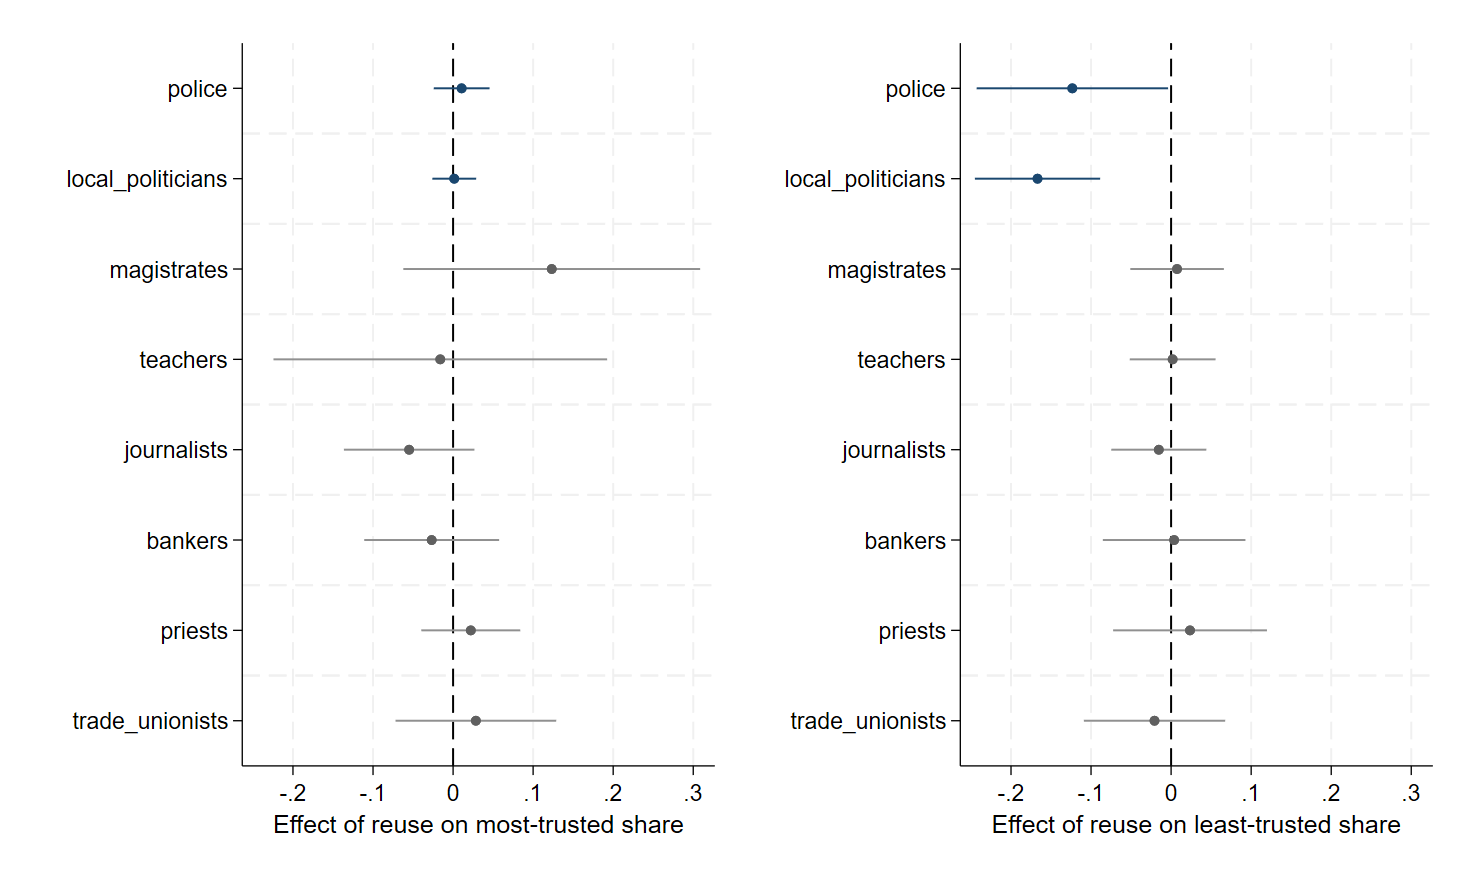
\includegraphics[width=15.4cm]{pictures_1/v48_coeffplot.png} }}%
	\caption{Estimated effects of repurposing practices on students' level of trust in several institutional bodies. Each point reports the effect of repurpose on the share of students level of trust, estimated from separate regressions that include school and year fixed effects, and are weighted by the number of students. Standard errors are clustered at the school level. Results are significant at the 90\% confidence level.}
	
	\label{fig:jmp_trust2}
	%say that the new policy gave a new emotional wave on the reallocation in general
	
\end{figure}

		\begin{figure}[H]%
	\centering
	{{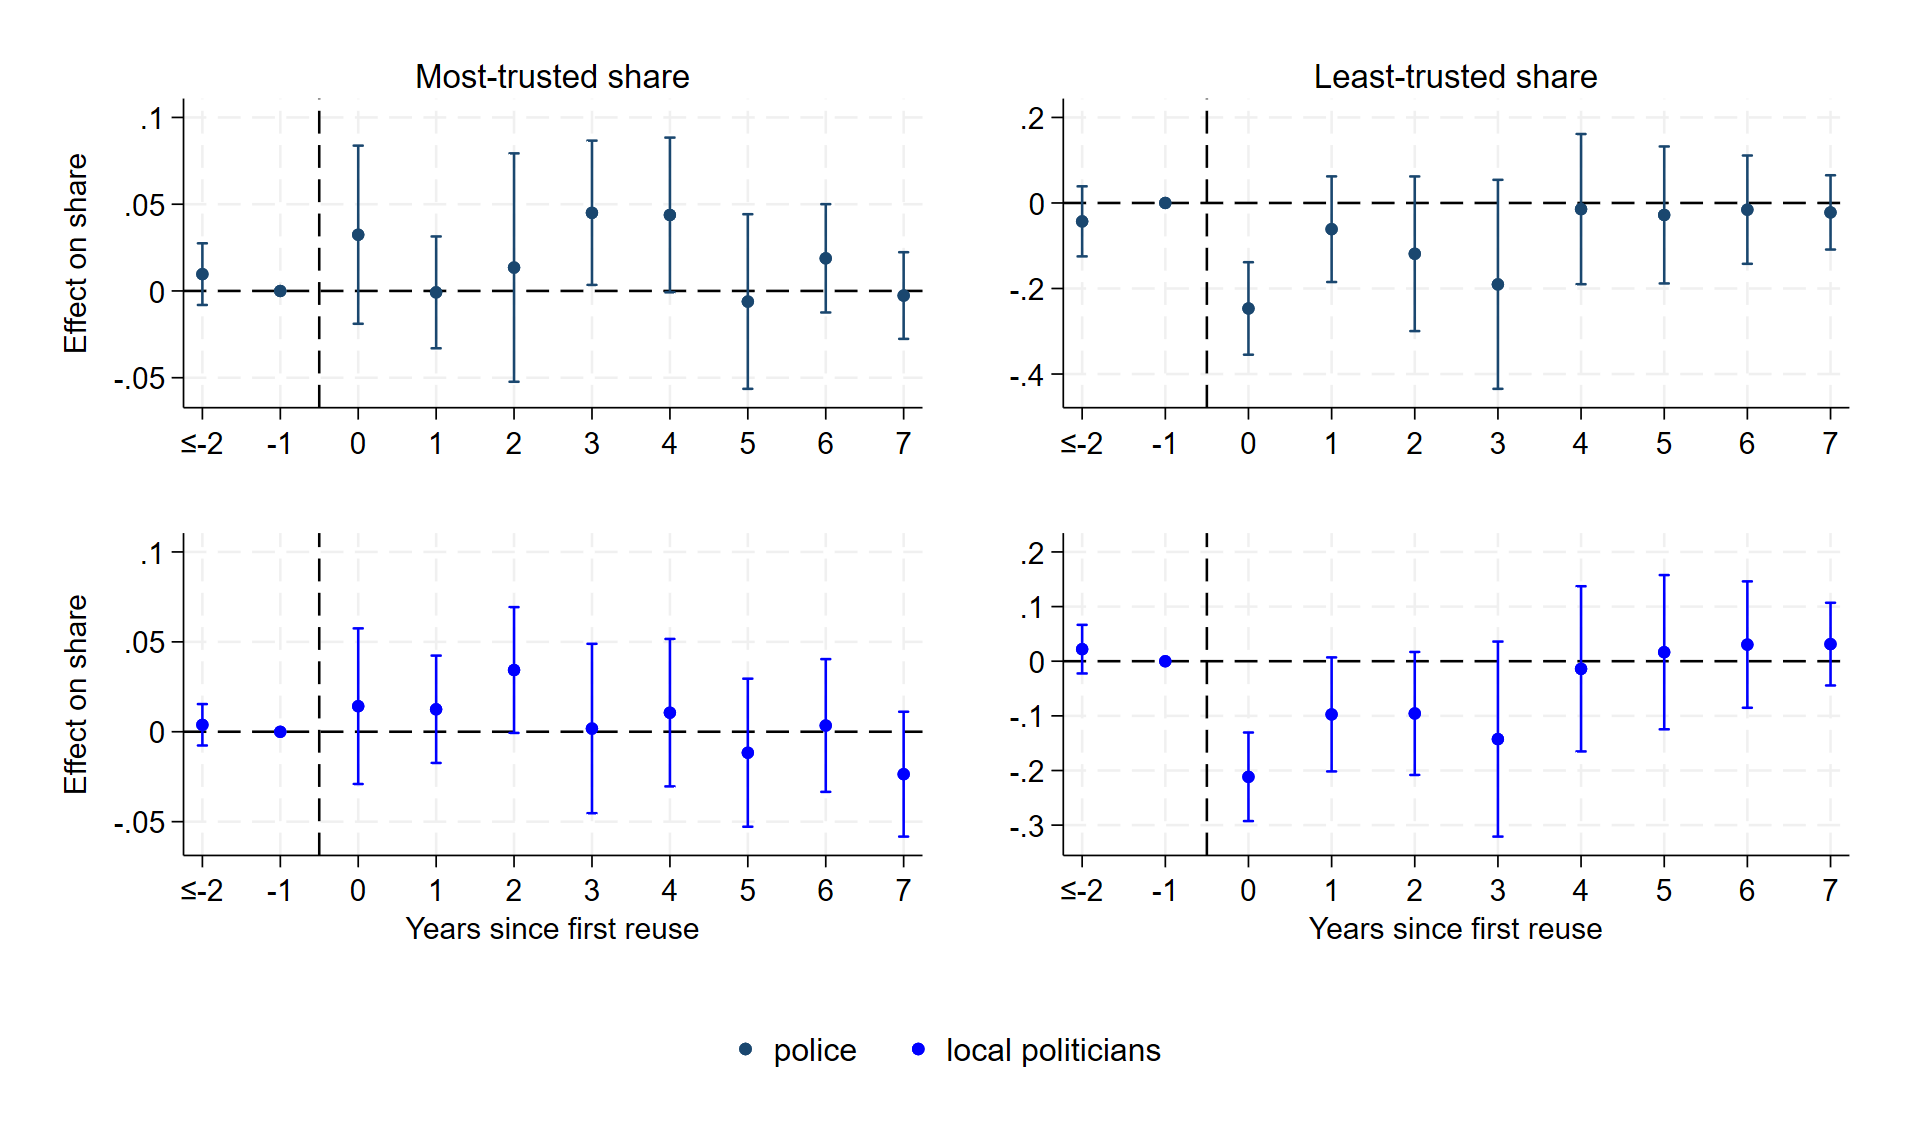
\includegraphics[width=15.4cm]{pictures_1/event_trust2.png} }}%
	\caption{Event studies of repurposing practices on students' level of trust in several institutional bodies. Each point reports the effect of repurpose on the share of students level of trust, estimated from separate regressions that include school and year fixed effects, and are weighted by the number of students. Standard errors are clustered at the school level. Results are significant at the 90\% confidence level.}
	
	\label{fig:jmp_trust2_ev}
	%say that the new policy gave a new emotional wave on the reallocation in general
	
\end{figure}
	


\section{Alternative Explanations}
\label{sec:jmp_altexpl}
The results so far are consistent with a belief-based channel and the repurposed properties signaling greater State's capacity. However, alternative mechanisms could produce the same pattern. I discuss and rule out here four alternative explanations. The first is that the dropout reduction reflects a lower cost of education, through the provision of additional educational activities at the repurposed sites. The second is that repurposing projects are part of a concurrent process of gentrification might be removing neighbourhood barriers to schooling, such as distance and transport costs. The remaining two concern the belief mechanism: even if we assume that the effect operates through students' perceptions, such a shift could reflect social-desirability pressure rather than a genuine change in perceived returns, or it could occur at the household level rather than at the student level. \\
\emph{Provision of educational support.} It is possible that the estimated reduction in the dropout rate reflects a decrease in the costs related to education. If repurposed properties offer specific educational activities such as after-school clubs and educational mentoring training, the decrease we observe in dropout rate might be the direct consequence of higher investments in keeping the youth in school in treated areas. Similar effects could be observed if repurposing projects are implemented as a part of broader educational or socially-focused programmes funded at the municipality or neighbourhood level. Figure~\ref{fig:jmp_cats_repurpose} already suggest this might not be the case. The activity decomposition shows that the effect is driven by properties hosting cultural activities, not those offering education or employment services. Here I take a further step and test whether repurposing projects affects students' academic performance, as measured by graduating grades. If the intervention operates by lowering the cost of schooling through the provision of additional educational resources, we could also expect an improvement in graduating grades alongside the reduction in dropout.\footnote{The prediction is not unambiguous. If the intervention retains students who would otherwise have dropped out, and these tend to be lower-performing, their inclusion in the pool of graduates could push average grades downward.} 

\begin{table}[H]
	\caption{Alternative explanations: the effect of repurposing properties on graduating grades.}
	\label{tab:alternative_expl_grad}
	\vspace{0.2cm}
	\centering
	\scalebox{0.75}{
		\begin{tabular}{p{14.835em}llllllll}
			\toprule
			\multicolumn{1}{l}{} & \multicolumn{1}{c}{(1)} & \multicolumn{1}{c}{(2)} & \multicolumn{1}{c}{(3)} & \multicolumn{1}{c}{(4)} & \multicolumn{1}{c}{(5)} & \multicolumn{1}{c}{(6)} & \multicolumn{1}{c}{(7)} & \multicolumn{1}{c}{(8)} \\
			\multicolumn{1}{l}{\textit{Dep. Variable}} & \multicolumn{4}{c}{\textbf{Grades from 60-69}} & \multicolumn{4}{c}{\textbf{Grades from 70-79}} \\
			\midrule
			\multicolumn{1}{l}{} & \multicolumn{1}{c}{} & \multicolumn{1}{c}{} & \multicolumn{1}{c}{} & \multicolumn{1}{c}{} & \multicolumn{1}{c}{} & \multicolumn{1}{c}{} & \multicolumn{1}{c}{} & \multicolumn{1}{c}{} \\
			\multicolumn{1}{l}{Repurpose = 1} & \multicolumn{1}{c}{-0.0174} & \multicolumn{1}{c}{-0.00997} & \multicolumn{1}{c}{-0.0161} & \multicolumn{1}{c}{-0.0104} & \multicolumn{1}{c}{0.00301} & \multicolumn{1}{c}{0.00593} & \multicolumn{1}{c}{0.00672} & \multicolumn{1}{c}{0.00638} \\
			\multicolumn{1}{l}{} & \multicolumn{1}{c}{(0.0143)} & \multicolumn{1}{c}{(0.0195)} & \multicolumn{1}{c}{(0.0161)} & \multicolumn{1}{c}{(0.0195)} & \multicolumn{1}{c}{(0.0101)} & \multicolumn{1}{c}{(0.0129)} & \multicolumn{1}{c}{(0.00997)} & \multicolumn{1}{c}{(0.0129)} \\
			\multicolumn{1}{l}{} & \multicolumn{1}{c}{} & \multicolumn{1}{c}{} & \multicolumn{1}{c}{} & \multicolumn{1}{c}{} & \multicolumn{1}{c}{} & \multicolumn{1}{c}{} & \multicolumn{1}{c}{} & \multicolumn{1}{c}{} \\
			\multicolumn{1}{l}{Observations} & \multicolumn{1}{c}{1,784} & \multicolumn{1}{c}{1,276} & \multicolumn{1}{c}{1,517} & \multicolumn{1}{c}{1,274} & \multicolumn{1}{c}{1,784} & \multicolumn{1}{c}{1,276} & \multicolumn{1}{c}{1,517} & \multicolumn{1}{c}{1,274} \\
			\multicolumn{1}{l}{R-squared} & \multicolumn{1}{c}{0.332} & \multicolumn{1}{c}{0.373} & \multicolumn{1}{c}{0.350} & \multicolumn{1}{c}{0.370} & \multicolumn{1}{c}{0.132} & \multicolumn{1}{c}{0.168} & \multicolumn{1}{c}{0.165} & \multicolumn{1}{c}{0.182} \\
			\multicolumn{1}{l}{Number of schools} & \multicolumn{1}{c}{251} & \multicolumn{1}{c}{234} & \multicolumn{1}{c}{243} & \multicolumn{1}{c}{234} & \multicolumn{1}{c}{251} & \multicolumn{1}{c}{234} & \multicolumn{1}{c}{243} & \multicolumn{1}{c}{234} \\
			\multicolumn{1}{l}{clustered SE} & \multicolumn{1}{c}{yes} & \multicolumn{1}{c}{yes} & \multicolumn{1}{c}{yes} & \multicolumn{1}{c}{yes} & \multicolumn{1}{c}{yes} & \multicolumn{1}{c}{yes} & \multicolumn{1}{c}{yes} & \multicolumn{1}{c}{yes} \\
			\multicolumn{1}{l}{school FE} & \multicolumn{1}{c}{yes} & \multicolumn{1}{c}{yes} & \multicolumn{1}{c}{yes} & \multicolumn{1}{c}{yes} & \multicolumn{1}{c}{yes} & \multicolumn{1}{c}{yes} & \multicolumn{1}{c}{yes} & \multicolumn{1}{c}{yes} \\
			\multicolumn{1}{l}{time FE} & \multicolumn{1}{c}{yes} & \multicolumn{1}{c}{yes} & \multicolumn{1}{c}{yes} & \multicolumn{1}{c}{yes} & \multicolumn{1}{c}{yes} & \multicolumn{1}{c}{yes} & \multicolumn{1}{c}{yes} & \multicolumn{1}{c}{yes} \\
			\multicolumn{1}{l}{migration} & \multicolumn{1}{c}{no} & \multicolumn{1}{c}{yes} & \multicolumn{1}{c}{no} & \multicolumn{1}{c}{yes} & \multicolumn{1}{c}{no} & \multicolumn{1}{c}{yes} & \multicolumn{1}{c}{no} & \multicolumn{1}{c}{yes} \\
			\multicolumn{1}{l}{retention} & \multicolumn{1}{c}{no} & \multicolumn{1}{c}{no} & \multicolumn{1}{c}{yes} & \multicolumn{1}{c}{yes} & \multicolumn{1}{c}{no} & \multicolumn{1}{c}{no} & \multicolumn{1}{c}{yes} & \multicolumn{1}{c}{yes} \\
			\multicolumn{1}{l}{Mean dep. var.} & \multicolumn{1}{c}{0.323} & \multicolumn{1}{c}{0.298} & \multicolumn{1}{c}{0.309} & \multicolumn{1}{c}{0.298} & \multicolumn{1}{c}{0.261} & \multicolumn{1}{c}{0.254} & \multicolumn{1}{c}{0.257} & \multicolumn{1}{c}{0.254} \\
			\midrule
			\multicolumn{1}{r}{} &       &       &       &       &       &       &       &  \\
			\midrule
			\multicolumn{1}{l}{\textit{Dep. Variable}} & \multicolumn{4}{c}{\textbf{Grades from 80-89}} & \multicolumn{4}{c}{\textbf{Grades from 90-100}} \\
			\midrule
			\multicolumn{1}{r}{} & \multicolumn{1}{c}{} & \multicolumn{1}{c}{} & \multicolumn{1}{c}{} & \multicolumn{1}{c}{} & \multicolumn{1}{c}{} & \multicolumn{1}{c}{} & \multicolumn{1}{c}{} & \multicolumn{1}{c}{} \\
			\multicolumn{1}{l}{Repurpose = 1} & \multicolumn{1}{c}{0.00945} & \multicolumn{1}{c}{0.00615} & \multicolumn{1}{c}{0.00816} & \multicolumn{1}{c}{0.00676} & \multicolumn{1}{c}{0.00681} & \multicolumn{1}{c}{0.00839} & \multicolumn{1}{c}{0.00429} & \multicolumn{1}{c}{0.00808} \\
			\multicolumn{1}{l}{} & \multicolumn{1}{c}{(0.0109)} & \multicolumn{1}{c}{(0.0137)} & \multicolumn{1}{c}{(0.0125)} & \multicolumn{1}{c}{(0.0136)} & \multicolumn{1}{c}{(0.00680)} & \multicolumn{1}{c}{(0.00861)} & \multicolumn{1}{c}{(0.00705)} & \multicolumn{1}{c}{(0.00859)} \\
			\multicolumn{1}{l}{} & \multicolumn{1}{c}{} & \multicolumn{1}{c}{} & \multicolumn{1}{c}{} & \multicolumn{1}{c}{} & \multicolumn{1}{c}{} & \multicolumn{1}{c}{} & \multicolumn{1}{c}{} & \multicolumn{1}{c}{} \\
			\multicolumn{1}{l}{Observations} & \multicolumn{1}{c}{1,784} & \multicolumn{1}{c}{1,276} & \multicolumn{1}{c}{1,517} & \multicolumn{1}{c}{1,274} & \multicolumn{1}{c}{1,784} & \multicolumn{1}{c}{1,276} & \multicolumn{1}{c}{1,517} & \multicolumn{1}{c}{1,274} \\
			\multicolumn{1}{l}{R-squared} & \multicolumn{1}{c}{0.069} & \multicolumn{1}{c}{0.092} & \multicolumn{1}{c}{0.078} & \multicolumn{1}{c}{0.099} & \multicolumn{1}{c}{0.324} & \multicolumn{1}{c}{0.331} & \multicolumn{1}{c}{0.329} & \multicolumn{1}{c}{0.333} \\
			\multicolumn{1}{l}{Number of schools} & \multicolumn{1}{c}{251} & \multicolumn{1}{c}{234} & \multicolumn{1}{c}{243} & \multicolumn{1}{c}{234} & \multicolumn{1}{c}{251} & \multicolumn{1}{c}{234} & \multicolumn{1}{c}{243} & \multicolumn{1}{c}{234} \\
			\multicolumn{1}{l}{clustered SE} & \multicolumn{1}{c}{yes} & \multicolumn{1}{c}{yes} & \multicolumn{1}{c}{yes} & \multicolumn{1}{c}{yes} & \multicolumn{1}{c}{yes} & \multicolumn{1}{c}{yes} & \multicolumn{1}{c}{yes} & \multicolumn{1}{c}{yes} \\
			\multicolumn{1}{l}{school FE} & \multicolumn{1}{c}{yes} & \multicolumn{1}{c}{yes} & \multicolumn{1}{c}{yes} & \multicolumn{1}{c}{yes} & \multicolumn{1}{c}{yes} & \multicolumn{1}{c}{yes} & \multicolumn{1}{c}{yes} & \multicolumn{1}{c}{yes} \\
			\multicolumn{1}{l}{time FE} & \multicolumn{1}{c}{yes} & \multicolumn{1}{c}{yes} & \multicolumn{1}{c}{yes} & \multicolumn{1}{c}{yes} & \multicolumn{1}{c}{yes} & \multicolumn{1}{c}{yes} & \multicolumn{1}{c}{yes} & \multicolumn{1}{c}{yes} \\
			\multicolumn{1}{l}{migration} & \multicolumn{1}{c}{no} & \multicolumn{1}{c}{yes} & \multicolumn{1}{c}{no} & \multicolumn{1}{c}{yes} & \multicolumn{1}{c}{no} & \multicolumn{1}{c}{yes} & \multicolumn{1}{c}{yes} & \multicolumn{1}{c}{yes} \\
			\multicolumn{1}{l}{retention} & \multicolumn{1}{c}{no} & \multicolumn{1}{c}{no} & \multicolumn{1}{c}{yes} & \multicolumn{1}{c}{yes} & \multicolumn{1}{c}{no} & \multicolumn{1}{c}{no} & \multicolumn{1}{c}{yes} & \multicolumn{1}{c}{yes} \\
			\multicolumn{1}{l}{Mean dep. var.} & \multicolumn{1}{c}{0.191} & \multicolumn{1}{c}{0.194} & \multicolumn{1}{c}{0.193} & \multicolumn{1}{c}{0.194} & \multicolumn{1}{c}{0.116} & \multicolumn{1}{c}{0.128} & \multicolumn{1}{c}{0.122} & \multicolumn{1}{c}{0.128} \\
			\midrule
			\multicolumn{9}{p{47.275em}}{Notes: TWFE model. The treatment variable is equal to 1 whenever there is at least one reused Mafia property within the school catchment area. Column (1) represents the baseline accounting for school and time fixed effects, while in Columns (2) and (3) I control for students' migration and grade retention rate, respectively. Column (4) reports the complete specification. Standard errors are clustered at the school level.} \\
		\end{tabular}%
	}
\end{table}

Table~\ref{tab:alternative_expl_grad} reports the effect of repurposing on the distribution of graduating grades, estimated separately for four grade brackets using the same specification as for dropout. The coefficient on repurposing is statistically insignificant in every bracket and across all specifications, indicating no detectable effect of the intervention on academic attainment. 
The pattern of signs is nonetheless informative for the composition concern raised above. Were the reduction in dropout retaining weaker students who would otherwise have left, their inclusion among graduates should raise the share in the lowest grade band. Instead, the point estimate for the lowest band (60–69) is, if anything, negative, while those for the higher bands are marginally positive. There is thus no evidence that the dropout effect operates by adding low-performing students to the graduate pool, nor that it raises attainment among those it retains. Altogether, the absence of any grade effect is inconsistent with an educational-inputs channel, which would predict measurable gains in performance, and consistent with a mechanism that operates on the decision to remain in school rather than on the students' performance itself. \\
Another related possibility is that the effect reflects not the activities on the repurposed properties themselves, but concurrent public investment in education and social inclusion in the same areas, which could reduce dropout through the same cost-of-schooling channel. I test this directly by controlling for other educational and social programmes implemented at the municipal level.\\
I collect data on the number of educational and social-cohesion projects implemented in each municipality and year from the Italian Department for Cohesion Policy \footnote{The data have been collected from \href{https://opencoesione.gov.it}{opencoesione.gov.it}}. The data cover projects targeting a range of developmental goals for local administrations between 2007 and 2022; I focus on education and social-inclusion projects, measured as the share of completed and ongoing projects relative to the total implemented in each municipality per year. Adding these as controls tests whether the estimated effect of repurposing reflects coincident policy activity rather than the intervention itself.
Table~\ref{tab:alternative_explanations} reports the results. The coefficient of the effect of repurposing properties is virtually unchanged across all specifications, ranging from 1.9 to 2.1 percentage points and remaining significant throughout, while neither educational nor social-inclusion projects show any detectable association with dropout rates (coefficients close to zero with large standard errors). The stability of the treatment coefficient indicates that the dropout reduction is specific to the repurposing intervention rather than a reflection of broader municipal development activity. These results suggest that repurposing effect might not be operating through the same channel as general educational provision. This is consistent with the activity decomposition, where the effect was driven by cultural rather than educational programmes.

\begin{table}[H]
	\caption{Alternative explanations: controlling for concurrent municipal programs}
	\label{tab:alternative_explanations}
	\vspace{0.2cm}
	\centering
	\scalebox{0.75}{
		\begin{tabular}{lcccc}
			\toprule
			& (1) & (2) & (3) & (4) \\
			& \multicolumn{4}{c}{\textbf{Dropout rate G11-G13}} \\
			\midrule
			Repurpose = 1 & -0.0193** & -0.0203** & -0.0198** & -0.0210** \\
			& (0.00903) & (0.00918) & (0.00867) & (0.00876) \\
			Educational programmes & -0.000777 & -0.00533 & 0.00289 & -0.00136 \\
			& (0.0146) & (0.0139) & (0.0151) & (0.0144) \\
			Social cohesion programmes & -0.000929 & -0.00334 & -0.00755 & -0.00869 \\
			& (0.0157) & (0.0153) & (0.0185) & (0.0184) \\
			\\
			Clustered SE & yes & yes & yes & yes \\
			Catchment school FE & yes & yes & yes & yes \\
			Time FE & yes & yes & yes & yes \\
			Migration controls & no & yes & no & yes \\
			Retention controls & no & no & yes & yes \\
			Observations & 1,269 & 1,265 & 1,248 & 1,246 \\
			Number of schools & 235 & 234 & 234 & 234 \\
			Mean dep. var. & 0.0538 & 0.0535 & 0.0530 & 0.0531 \\
			\midrule
			\multicolumn{5}{p{35em}}{Notes: TWFE model. The treatment variable is equal to 1 whenever there is at least one Mafia property within the school catchment area. Column (1) does not include controls while Columns (2) includes controls for migration. Column (3) includes only the controls for grade retention rate, while Column (4) include them all. Standard errors are clustered at the school level.} \\
		\end{tabular}%
	}
\end{table}


\emph{Mafia presence and recruitment.} The repurpose of Mafia properties represents the final stage of the CRR policy, which requires first confiscating and then reallocating confiscated assets under the jurisdiction of local authorities. \citet{boeri_localized_2023} demonstrate that the confiscation of nearby Mafia properties depresses housing prices by signalling the local presence of the Mafia, while reallocation sends the opposite signal, restoring property values. A potential concern is therefore that my treatment variable captures a recovery process following multiple confiscations that negatively affected neighbourhoods, reduced local economic activity, and contributed to higher dropout rates.
\par\medskip
A related concern is that the repurpose treatment merely captures dropout reductions driven by the reallocation stage rather than the repurposing itself. I argue this is implausible for two reasons. First, reallocation is a purely administrative process whereby confiscated properties are formally transferred to local authorities. While this may signal a municipality's intention to repurpose former Mafia assets, it generates no tangible changes at the community level and no social activity that could plausibly alter youth behaviour or educational decisions. Second, Table~\ref{tab:jmp_reallocation} provides direct empirical evidence: Columns (3) and (4) show that reallocation alone has no independent effect on dropout rates, with coefficients close to zero and consistently insignificant across specifications. Columns (5) and (6) show that the reuse coefficient remains stable in magnitude and statistically significant at the 5\% level even after controlling for reallocations. Taken together, this evidence supports the interpretation that meaningful educational impacts arise when properties are actively repurposed for community use, rather than simply transferred to public ownership. The event study reported in Figure~\ref{fig:es_reallocation} corroborates these findings, showing no differential pre-trends and estimates closely in line with the main specification.

\begin{table}[H]
	\caption{Impact of reusing Mafia real estate on the share of students dropping out at the age of 16 - including previous policy stage} % Table label
	\label{tab:jmp_reallocation}
	\vspace{0.2cm}
	\centering
	\scalebox{0.75}{
		\begin{tabular}{p{7.39em}llllll}
			\toprule
			\multicolumn{1}{l}{} & \multicolumn{1}{c}{(1)} & \multicolumn{1}{c}{(2)} & \multicolumn{1}{c}{(3)} & \multicolumn{1}{c}{(4)} & \multicolumn{1}{c}{(5)} & \multicolumn{1}{c}{(6)} \\
			\multicolumn{1}{r}{} & \multicolumn{6}{c}{\textbf{Dropout rate G11-G13}} \\
			\midrule
			\multicolumn{1}{l}{} & \multicolumn{1}{c}{} & \multicolumn{1}{c}{} & \multicolumn{1}{c}{} & \multicolumn{1}{c}{} & \multicolumn{1}{c}{} & \multicolumn{1}{c}{} \\
			\multicolumn{1}{l}{Reuse = 1} & \multicolumn{1}{c}{-0.0192**} & \multicolumn{1}{c}{-0.0196**} & \multicolumn{1}{c}{} & \multicolumn{1}{c}{} & \multicolumn{1}{c}{-0.0193**} & \multicolumn{1}{c}{-0.0199**} \\
			\multicolumn{1}{l}{} & \multicolumn{1}{c}{(0.00934)} & \multicolumn{1}{c}{(0.00943)} & \multicolumn{1}{c}{} & \multicolumn{1}{c}{} & \multicolumn{1}{c}{(0.00936)} & \multicolumn{1}{c}{(0.00948)} \\
			\multicolumn{1}{l}{Reallocation = 1} & \multicolumn{1}{c}{} & \multicolumn{1}{c}{} & \multicolumn{1}{c}{0.00477} & \multicolumn{1}{c}{-0.000235} & \multicolumn{1}{c}{0.00290} & \multicolumn{1}{c}{-0.00238} \\
			\multicolumn{1}{l}{} & \multicolumn{1}{c}{} & \multicolumn{1}{c}{} & \multicolumn{1}{c}{(0.00653)} & \multicolumn{1}{c}{(0.0101)} & \multicolumn{1}{c}{(0.00653)} & \multicolumn{1}{c}{(0.0102)} \\
			\multicolumn{1}{l}{} & \multicolumn{1}{c}{} & \multicolumn{1}{c}{} & \multicolumn{1}{c}{} & \multicolumn{1}{c}{} & \multicolumn{1}{c}{} & \multicolumn{1}{c}{} \\
			\multicolumn{1}{l}{clustered SE} & \multicolumn{1}{c}{yes} & \multicolumn{1}{c}{yes} & \multicolumn{1}{c}{yes} & \multicolumn{1}{c}{yes} & \multicolumn{1}{c}{yes} & \multicolumn{1}{c}{yes} \\
			\multicolumn{1}{l}{school FE} & \multicolumn{1}{c}{yes} & \multicolumn{1}{c}{yes} & \multicolumn{1}{c}{yes} & \multicolumn{1}{c}{yes} & \multicolumn{1}{c}{yes} & \multicolumn{1}{c}{yes} \\
			\multicolumn{1}{l}{time FE} & \multicolumn{1}{c}{yes} & \multicolumn{1}{c}{yes} & \multicolumn{1}{c}{yes} & \multicolumn{1}{c}{yes} & \multicolumn{1}{c}{yes} & \multicolumn{1}{c}{yes} \\
			\multicolumn{1}{l}{migration} & \multicolumn{1}{c}{no} & \multicolumn{1}{c}{yes} & \multicolumn{1}{c}{no} & \multicolumn{1}{c}{yes} & \multicolumn{1}{c}{no} & \multicolumn{1}{c}{yes} \\
			\multicolumn{1}{l}{retention} & \multicolumn{1}{c}{no} & \multicolumn{1}{c}{yes} & \multicolumn{1}{c}{no} & \multicolumn{1}{c}{yes} & \multicolumn{1}{c}{no} & \multicolumn{1}{c}{yes} \\
			\multicolumn{1}{l}{Observations} & \multicolumn{1}{c}{1,296} & \multicolumn{1}{c}{1,272} & \multicolumn{1}{c}{1,286} & \multicolumn{1}{c}{1,262} & \multicolumn{1}{c}{1,286} & \multicolumn{1}{c}{1,262} \\
			\multicolumn{1}{l}{Number of schools} & \multicolumn{1}{c}{235} & \multicolumn{1}{c}{234} & \multicolumn{1}{c}{233} & \multicolumn{1}{c}{232} & \multicolumn{1}{c}{233} & \multicolumn{1}{c}{232} \\
			\multicolumn{1}{l}{Mean dep. var.} & \multicolumn{1}{c}{0.0537} & \multicolumn{1}{c}{0.0531} & \multicolumn{1}{c}{0.0537} & \multicolumn{1}{c}{0.0531} & \multicolumn{1}{c}{0.0537} & \multicolumn{1}{c}{0.0531} \\
			\midrule
			\multicolumn{7}{p{37.39em}}{Notes: TWFE model. The treatment variable is equal to 1 whenever there is at least one reused Mafia property within the school catchment area. Standard errors are clustered at the school level.} \\
		\end{tabular}%
	}
\end{table}

\emph{Gentrification and neighbourhood effects.} A second explanation is that repurposing former Mafia properties is part of a broader gentrification process occurring in treated areas. Regenerating a neighbourhood could lower local barriers to schooling, and the estimated effect would then reflect this upgrading rather than the Mafia-related intervention itself. \\
I test this using a triple difference-in-differences design that interacts the treatment with local property values, proxied by average rental prices per square metre at the neighbourhood level. If the effect operates through neighbourhood upgrading, it should be stronger where property values are rising. The specification is:
\begin{equation} \label{continuous_spec}
	\begin{aligned}
		DropoutG11\text{-}G13_{cnmt} =\; & \beta_1 Repurpose_{ct} \times Prices_{nt} \\
		& + \beta_2 Repurpose_{c} + \beta_3 Prices_{n} \\
		& + \beta_4 X'_{ct} + \delta_c + \eta_t + \epsilon_{cnmt}
	\end{aligned}
\end{equation}

where $DropoutG11-G13_{cnmt}$ is the main outcome as specified before, and $Reuse$ is the main treatment dummy equal to 1 whenever there is at least one reused property in the school catchment area $c$ in time $t$, and 0 otherwise. $Prices$ measures the average rental prices in neighbourhood $n$ at time $t$, while $\beta_1$ is the coefficient of interest which captures how the impact of repurposed Mafia properties on dropout rates varies with local property price dynamics. $X'_{c,t}$ is a vector of time-varying community-level variables controlling for students' migration and grade retention dynamics. $\delta_c$ is school fixed effects and $\eta_t$ is time fixed effects. \\
If the main effect operates through the upgrading and gentrification of the neighbourhood, I would expect the effect of treatment to be stronger in areas experiencing increases in rental prices. Table~\ref{tab:jmp_gentrification} shows the results; the coefficient of the interaction term is very close to zero and not statistically significant, making the effect of rental price changes on dropout rates virtually identical in areas with and without repurposed properties. Moreover, the results are robust to the inclusion of migration and grade retention controls. These results support the argument that specific activities and programs do not reduce dropout rates through a general gentrification effect at the neighbourhood level.

\begin{table}[H]
	\caption{Impact of reusing Mafia real estate and NGO presence on dropout rates for G11-G13 interacted with rent price} % Table label
	\label{tab:jmp_gentrification}
	\vspace{0.2cm}
	\centering
	\scalebox{0.85}{
		\begin{tabular}{p{7.39em}llll}
			\toprule
			\multicolumn{1}{l}{} & \multicolumn{1}{c}{(1)} & \multicolumn{1}{c}{(2)} & \multicolumn{1}{c}{(3)} & \multicolumn{1}{c}{(4)} \\
			\multicolumn{1}{r}{} & \multicolumn{4}{c}{\textbf{Dropout rate G11-G13}} \\
			\midrule
			\multicolumn{1}{l}{} & \multicolumn{1}{c}{} & \multicolumn{1}{c}{} & \multicolumn{1}{c}{} & \multicolumn{1}{c}{} \\
			\multicolumn{1}{l}{Repurpose = 1} & \multicolumn{1}{c}{-0.0144} & \multicolumn{1}{c}{-0.0208} & \multicolumn{1}{c}{-0.0137} & \multicolumn{1}{c}{-0.0213} \\
			\multicolumn{1}{l}{} & \multicolumn{1}{c}{(0.0375)} & \multicolumn{1}{c}{(0.0383)} & \multicolumn{1}{c}{(0.0372)} & \multicolumn{1}{c}{(0.0380)} \\
			\multicolumn{1}{l}{Rental Prices} & \multicolumn{1}{c}{-0.000801} & \multicolumn{1}{c}{-0.00469} & \multicolumn{1}{c}{-0.00128} & \multicolumn{1}{c}{-0.00475} \\
			\multicolumn{1}{l}{} & \multicolumn{1}{c}{(0.00709)} & \multicolumn{1}{c}{(0.00695)} & \multicolumn{1}{c}{(0.00691)} & \multicolumn{1}{c}{(0.00681)} \\
			\multicolumn{1}{l}{Repurpose =1 $\times$ Rental Prices} & \multicolumn{1}{c}{-0.000566} & \multicolumn{1}{c}{0.000127} & \multicolumn{1}{c}{-0.000626} & \multicolumn{1}{c}{0.000191} \\
			\multicolumn{1}{l}{} & \multicolumn{1}{c}{(0.00382)} & \multicolumn{1}{c}{(0.00390)} & \multicolumn{1}{c}{(0.00375)} & \multicolumn{1}{c}{(0.00383)} \\
			\multicolumn{1}{l}{} & \multicolumn{1}{c}{} & \multicolumn{1}{c}{} & \multicolumn{1}{c}{} & \multicolumn{1}{c}{} \\
			\multicolumn{1}{l}{clustered SE} & \multicolumn{1}{c}{yes} & \multicolumn{1}{c}{yes} & \multicolumn{1}{c}{yes} & \multicolumn{1}{c}{yes} \\
			\multicolumn{1}{l}{ school FE} & \multicolumn{1}{c}{yes} & \multicolumn{1}{c}{yes} & \multicolumn{1}{c}{yes} & \multicolumn{1}{c}{yes} \\
			\multicolumn{1}{l}{time FE} & \multicolumn{1}{c}{yes} & \multicolumn{1}{c}{yes} & \multicolumn{1}{c}{yes} & \multicolumn{1}{c}{yes} \\
			\multicolumn{1}{l}{migration} & \multicolumn{1}{c}{no} & \multicolumn{1}{c}{yes} & \multicolumn{1}{c}{no} & \multicolumn{1}{c}{yes} \\
			\multicolumn{1}{l}{retention} & \multicolumn{1}{c}{no} & \multicolumn{1}{c}{no} & \multicolumn{1}{c}{yes} & \multicolumn{1}{c}{yes} \\
			\multicolumn{1}{l}{Observations} & \multicolumn{1}{c}{1,296} & \multicolumn{1}{c}{1,292} & \multicolumn{1}{c}{1,274} & \multicolumn{1}{c}{1,272} \\
			\multicolumn{1}{l}{Number of schools} & \multicolumn{1}{c}{235} & \multicolumn{1}{c}{234} & \multicolumn{1}{c}{234} & \multicolumn{1}{c}{234} \\
			\multicolumn{1}{l}{Mean dep. var.} & \multicolumn{1}{c}{0.0537} & \multicolumn{1}{c}{0.0534} & \multicolumn{1}{c}{0.0530} & \multicolumn{1}{c}{0.0531} \\
			\midrule
			\multicolumn{5}{p{37.61em}}{Notes: TWFE model. The treatment variable is equal to 1 whenever there is at least one Mafia property within the school catchment area. Column (1) does not include controls while Columns (2) includes controls for migration. Column (3) includes only the controls for grade retention rate, while Column (4) include them all. Standard errors are clustered at the school level.} \\
		\end{tabular}%
	}
\end{table}



\FloatBarrier
\section{Robustness Checks}
\label{sec:jmp_robustness}
The estimated effects are robust to a series of specification checks and alternative treatment assumptions. This section proceeds as follows. First, I test for additional confounding factors that may represent sources of omitted variable bias. Second, I investigate whether pre-treatment reallocations or anticipation effects could be confounding the estimated results. Third, I assess whether the treatment allocation is subject to spatial selection bias. Fourth, I test for spatial spillover effects onto neighbouring schools. \par 
\medskip
\FloatBarrier
\subsection{Selection Bias}
\label{sec:jmp_ovb}


\emph{Treated versus not-yet-treated schools.} A primary concern is that never-treated schools may be fundamentally different from eventually-treated schools. Although Table~\ref{tab:jmp_desc_stats} shows broadly comparable pre-treatment characteristics across groups, the never-treated areas may differ along unobserved dimensions, such as the degree of institutional engagement with confiscated assets and the level of local support for antimafia policies, making them an inappropriate control group. To address this, I only exploit the timing of the treatment by restricting the comparison to treated and not-yet-treated schools, excluding never-treated units entirely. This ensures that the control group consists only of schools that eventually receive treatment, and therefore plausibly belong to the same population of Mafia-affected areas undergoing institutional repurpose processes. \\
Table~\ref{tab:jmp_selection_bias} reports the results from this restricted sample. The estimates are remarkably stable and, if anything, slightly larger in magnitude than the main specification, while remain statistically significant at the 5 percent level throughout. This stability is reassuring on two fronts. First, it suggests that the main results are not inflated by the inclusion of never-treated schools as being structurally different from treated areas. Second, the fact that the effect is preserved and marginally strengthened  when identification comes solely from variation in treatment timing among eventually-treated schools lends further credibility to the causal interpretation. The reduction in the number of schools from 232 to approximately 182 does not meaningfully affect precision, indicating that the never-treated units are not driving the main statistical power of the baseline estimates.

\begin{table}[H]
	\caption{Impact of reusing Mafia real estate on the share of students dropping out at the age of 16 - different catchment areas assumptions} % Table label
	\label{tab:jmp_selection_bias}
	\vspace{0.2cm}
	\centering
	\scalebox{0.85}{
		\begin{tabular}{p{8.11em}llll}
			\toprule
			\multicolumn{1}{l}{} & \multicolumn{1}{c}{(1)} & \multicolumn{1}{c}{(2)} & \multicolumn{1}{c}{(3)} & \multicolumn{1}{c}{(4)} \\
			\multicolumn{1}{r}{} & \multicolumn{4}{c}{\textbf{Dropout rate G11-G13}} \\
			\midrule
			\multicolumn{1}{l}{} & \multicolumn{1}{c}{} & \multicolumn{1}{c}{} & \multicolumn{1}{c}{} & \multicolumn{1}{c}{} \\
			\multicolumn{1}{l}{Repurpose = 1 } & \multicolumn{1}{c}{-0.0220**} & \multicolumn{1}{c}{-0.0232**} & \multicolumn{1}{c}{-0.0212**} & \multicolumn{1}{c}{-0.0227**} \\
			\multicolumn{1}{l}{} & \multicolumn{1}{c}{(0.00951)} & \multicolumn{1}{c}{(0.00965)} & \multicolumn{1}{c}{(0.00956)} & \multicolumn{1}{c}{(0.00968)} \\
			\multicolumn{1}{l}{} & \multicolumn{1}{c}{} & \multicolumn{1}{c}{} & \multicolumn{1}{c}{} & \multicolumn{1}{c}{} \\
			\multicolumn{1}{l}{clustered SE} & \multicolumn{1}{c}{yes} & \multicolumn{1}{c}{yes} & \multicolumn{1}{c}{yes} & \multicolumn{1}{c}{yes} \\
			\multicolumn{1}{l}{catchment school FE} & \multicolumn{1}{c}{yes} & \multicolumn{1}{c}{yes} & \multicolumn{1}{c}{yes} & \multicolumn{1}{c}{yes} \\
			\multicolumn{1}{l}{time FE} & \multicolumn{1}{c}{yes} & \multicolumn{1}{c}{yes} & \multicolumn{1}{c}{yes} & \multicolumn{1}{c}{yes} \\
			\multicolumn{1}{l}{migration} & \multicolumn{1}{c}{no} & \multicolumn{1}{c}{yes} & \multicolumn{1}{c}{no} & \multicolumn{1}{c}{yes} \\
			\multicolumn{1}{l}{retention} & \multicolumn{1}{c}{no} & \multicolumn{1}{c}{no} & \multicolumn{1}{c}{yes} & \multicolumn{1}{c}{yes} \\
			\multicolumn{1}{l}{Observations} & \multicolumn{1}{c}{1,028} & \multicolumn{1}{c}{1,025} & \multicolumn{1}{c}{1,014} & \multicolumn{1}{c}{1,013} \\
			\multicolumn{1}{l}{R-squared} & \multicolumn{1}{c}{0.094} & \multicolumn{1}{c}{0.108} & \multicolumn{1}{c}{0.092} & \multicolumn{1}{c}{0.106} \\
			\multicolumn{1}{l}{Number of schools} & \multicolumn{1}{c}{183} & \multicolumn{1}{c}{182} & \multicolumn{1}{c}{182} & \multicolumn{1}{c}{182} \\
			\multicolumn{1}{l}{Mean dep. var.} & \multicolumn{1}{c}{0.0566} & \multicolumn{1}{c}{0.0562} & \multicolumn{1}{c}{0.0558} & \multicolumn{1}{c}{0.0558} \\
			\midrule
			\multicolumn{5}{p{28.11em}}{Notes: TWFE model. The treatment variable is equal to 1 whenever there is at least one reused Mafia property within the school catchment area. Column (1) represents the baseline accounting for school and time fixed effects, while in Columns (2) and (3) I control for students' migration and grade retention rate, respectively. Column (4) reports the complete specification. Standard errors are clustered at the school level.} \\
		\end{tabular}%
	}
\end{table}


\emph{The presence of amenities.} In the main specification, I control for unit-specific and time-specific characteristics, as well as the time-varying rates of retention and migration among students. By controlling for these factors, I find no pre-trends in any of the estimated event study. Nevertheless, previous trends in the presence of NGOs and civic engagement might play a substantial role in how and when the policy is implemented locally. A natural question arises when interpreting the effects of the policy on dropout rate: is there something uniquely valuable about conducting activities in former Mafia properties, or would any NGO operating in the area produce similar reductions in dropout rates? To disentangle the specific contribution of repurposed properties from the broader effect of civil society presence, I test whether the main estimates are sensitive to controlling for the number of NGOs active within each school's catchment area. If the observed effects were simply driven by the availability of social services nearby, regardless of whether they operate from repurposed Mafia properties, the main coefficient should diminish substantially once I account for the local presence of NGOs. Conversely, if the main coefficient remains stable while the proxy for the presence of NGOs shows little independent effect, this would suggest that the symbolic and contextual significance of operating within former Mafia properties generates distinctive value that conventional NGO activities might not be able to replicate.
Table~\ref{tab:jmp_ngo_presence} supports this last interpretation. Columns (2) and (5) show that the presence of other NGOs in school catchment areas has negligible and statistically insignificant effects on dropout rates, indicating that general NGO activity alone does not meaningfully reduce educational dropout. Moreover, the repurposing effect remains remarkably stable when controlling for NGO presence. Comparing the baseline specifications in columns (1) and (4) with the full specifications in columns (3) and (6), the reuse coefficients are virtually unchanged in magnitude and remain statistically significant at the 5\% level throughout. These results provide compelling evidence that the observed effects stem not from general social service provision in the area, but from the particular significance of conducting activities within former Mafia properties. I further confirm the absence of differential pre-trends while controlling for the presence of NGOs, with the corresponding event study presented in Figure~\ref{fig:es_alt_ngo}. \par
\begin{table}[H]
	\caption{Impact of reusing Mafia real estate and NGO presence on dropout rates for G11-G13} % Table label
	\label{tab:jmp_ngo_presence}
	\vspace{0.2cm}
	\centering
	\scalebox{0.78}{
		\begin{tabular}{p{4.055em}llllll}
			\toprule
			\multicolumn{1}{l}{} & \multicolumn{1}{c}{(1)} & \multicolumn{1}{c}{(2)} & \multicolumn{1}{c}{(3)} & \multicolumn{1}{c}{(4)} & \multicolumn{1}{c}{(5)} & \multicolumn{1}{c}{(6)} \\
			\multicolumn{1}{r}{} & \multicolumn{6}{c}{Dropout rate G11-G13} \\
			\midrule
			\multicolumn{1}{l}{} & \multicolumn{1}{c}{} & \multicolumn{1}{c}{} & \multicolumn{1}{c}{} & \multicolumn{1}{c}{} & \multicolumn{1}{c}{} & \multicolumn{1}{c}{} \\
			
			\multicolumn{1}{l}{Reuse = 1} & \multicolumn{1}{c}{-0.0192**} & \multicolumn{1}{c}{} & \multicolumn{1}{c}{-0.0191**} & \multicolumn{1}{c}{-0.0196**} & \multicolumn{1}{c}{} & \multicolumn{1}{c}{-0.0194**} \\
			\multicolumn{1}{l}{} & \multicolumn{1}{c}{(0.00934)} & \multicolumn{1}{c}{} & \multicolumn{1}{c}{(0.00960)} & \multicolumn{1}{c}{(0.00945)} & \multicolumn{1}{c}{} & \multicolumn{1}{c}{(0.00963)} \\
			\multicolumn{1}{l}{NGOs presence} & \multicolumn{1}{c}{} & \multicolumn{1}{c}{-0.000590} & \multicolumn{1}{c}{-0.000626} & \multicolumn{1}{c}{} & \multicolumn{1}{c}{-0.000542} & \multicolumn{1}{c}{-0.000583} \\
			\multicolumn{1}{l}{} & \multicolumn{1}{c}{} & \multicolumn{1}{c}{(0.000392)} & \multicolumn{1}{c}{(0.000389)} & \multicolumn{1}{c}{} & \multicolumn{1}{c}{(0.000351)} & \multicolumn{1}{c}{(0.000354)} \\
			\multicolumn{1}{l}{} & \multicolumn{1}{c}{} & \multicolumn{1}{c}{} & \multicolumn{1}{c}{} & \multicolumn{1}{c}{} & \multicolumn{1}{c}{} & \multicolumn{1}{c}{} \\
			\multicolumn{1}{l}{clustered SE} & \multicolumn{1}{c}{yes} & \multicolumn{1}{c}{yes} & \multicolumn{1}{c}{yes} & \multicolumn{1}{c}{yes} & \multicolumn{1}{c}{yes} & \multicolumn{1}{c}{yes} \\
			\multicolumn{1}{l}{catchment school FE} & \multicolumn{1}{c}{yes} & \multicolumn{1}{c}{yes} & \multicolumn{1}{c}{yes} & \multicolumn{1}{c}{yes} & \multicolumn{1}{c}{yes} & \multicolumn{1}{c}{yes} \\
			\multicolumn{1}{l}{time FE} & \multicolumn{1}{c}{yes} & \multicolumn{1}{c}{yes} & \multicolumn{1}{c}{yes} & \multicolumn{1}{c}{yes} & \multicolumn{1}{c}{yes} & \multicolumn{1}{c}{yes} \\
			\multicolumn{1}{l}{migration} & \multicolumn{1}{c}{no} & \multicolumn{1}{c}{yes} & \multicolumn{1}{c}{no} & \multicolumn{1}{c}{yes} & \multicolumn{1}{c}{no} & \multicolumn{1}{c}{yes} \\
			\multicolumn{1}{l}{retention} & \multicolumn{1}{c}{no} & \multicolumn{1}{c}{yes} & \multicolumn{1}{c}{no} & \multicolumn{1}{c}{yes} & \multicolumn{1}{c}{no} & \multicolumn{1}{c}{yes} \\
			\multicolumn{1}{l}{Observations} & \multicolumn{1}{c}{1,296} & \multicolumn{1}{c}{1,487} & \multicolumn{1}{c}{1,296} & \multicolumn{1}{c}{1,272} & \multicolumn{1}{c}{1,447} & \multicolumn{1}{c}{1,272} \\
			\multicolumn{1}{l}{Number of schools} & \multicolumn{1}{c}{235} & \multicolumn{1}{c}{293} & \multicolumn{1}{c}{235} & \multicolumn{1}{c}{234} & \multicolumn{1}{c}{288} & \multicolumn{1}{c}{234} \\
			\multicolumn{1}{l}{Mean dep. var.} & \multicolumn{1}{c}{0.0537} & \multicolumn{1}{c}{0.0552} & \multicolumn{1}{c}{0.0537} & \multicolumn{1}{c}{0.0531} & \multicolumn{1}{c}{0.0541} & \multicolumn{1}{c}{0.0531} \\
			\midrule
			\multicolumn{7}{p{43.385em}}{Notes: TWFE model. The treatment variable is equal to 1 whenever there is at least one Mafia property within the school catchment area. Columns (1), (3), and (5) do not include controls while Columns (2), (4), and (6) include them all. Standard errors are clustered at the school level.} \\
		\end{tabular}%
	}
\end{table}
\FloatBarrier

\emph{Capacity-weighted catchment areas.} A further concern relates to spatial selection bias arising from the method used to construct school catchment areas. Treatment allocation may be sensitive to the baseline assumption that students attend their geographically closest school regardless of its size or capacity. Since catchment areas are constructed by assigning each census block to the nearest school, the boundaries between adjacent catchment areas are determined purely by proximity. This rule may misclassify treatment status for schools near those boundaries: if larger schools in practice serve students living closer to a neighbouring smaller school, then a reused property near such a boundary could be assigned to the wrong catchment area, generating a measurement error in treatment that is correlated with school characteristics.
I re-estimate the main results under alternative assumptions about the construction of schools' catchment areas. If the effect were spuriously driven by the specific rule used to assign treatment status, changing that rule should produce meaningfully different treatment allocations and consequently different estimates. Specifically, I weight the Euclidean distance between each census block and the closest school by the school capacity, namely the enrollment in the first year for each school measured at the baseline. This capacity-weighted approach allows larger schools to draw students from greater distances and have more extensive catchment areas; this provides a more realistic representation of how students are distributed across urban areas \citep{pearce_techniques_2000}.\footnote{Appendix~\ref{sec:jmp_app_D} explains in detail how the areas have been computed.} 
Under the capacity-weighted construction, only 18 schools switch treatment status relative to the baseline assignment. The small number of switchers is itself reassuring, suggesting that the two approaches yield largely consistent treatment allocations. To further ensure that the main results are not driven by schools with inherently ambiguous treatment assignment, I re-estimate the main specification excluding these 18 schools. Table~\ref{tab:jmp_catchment_alt} shows that the coefficients of interest are virtually unchanged across all specifications, whether estimated on the full sample or on the restricted sample. The stability of the estimates across both the alternative weighting scheme and the restricted sample jointly suggests that the treatment effect is not an artifact of how catchment areas are constructed. The somewhat wider confidence intervals in the restricted sample are expected given the reduction in sample size, and if anything underscore the importance of retaining the full sample for statistical precision without compromising identification. \par

\begin{table}[H]
	\caption{Impact of reusing Mafia real estate on the share of students dropping out at the age of 16 - capacity-weighted catchment areas} % Table label
	\label{tab:jmp_catchment_alt}
	\vspace{0.2cm}
	\centering
	\scalebox{0.85}{
		\begin{tabular}{p{12.39em}llll}
			\toprule
			\multicolumn{1}{l}{} & \multicolumn{1}{c}{(1)} & \multicolumn{1}{c}{(2)} & \multicolumn{1}{c}{(3)} & \multicolumn{1}{c}{(4)} \\
			\multicolumn{1}{l}{Dep Var: Dropout rate G11-13} & \multicolumn{1}{c}{\textbf{All sample}} & \multicolumn{1}{c}{\textbf{Non-switchers only}} & \multicolumn{1}{c}{\textbf{All sample}} & \multicolumn{1}{c}{\textbf{Non-switchers only}} \\
			\midrule
			\multicolumn{1}{l}{} & \multicolumn{1}{c}{} & \multicolumn{1}{c}{} & \multicolumn{1}{c}{} & \multicolumn{1}{c}{} \\
			\multicolumn{1}{l}{Reuse = 1} & \multicolumn{1}{c}{-0.0192**} & \multicolumn{1}{c}{-0.0206*} & \multicolumn{1}{c}{-0.0196**} & \multicolumn{1}{c}{-0.0207*} \\
			\multicolumn{1}{l}{} & \multicolumn{1}{c}{(0.00934)} & \multicolumn{1}{c}{(0.0122)} & \multicolumn{1}{c}{(0.00943)} & \multicolumn{1}{c}{(0.0123)} \\
			\multicolumn{1}{l}{} & \multicolumn{1}{c}{} & \multicolumn{1}{c}{} & \multicolumn{1}{c}{} & \multicolumn{1}{c}{} \\
			\multicolumn{1}{l}{clustered SE} & \multicolumn{1}{c}{yes} & \multicolumn{1}{c}{yes} & \multicolumn{1}{c}{yes} & \multicolumn{1}{c}{yes} \\
			\multicolumn{1}{l}{school FE} & \multicolumn{1}{c}{yes} & \multicolumn{1}{c}{yes} & \multicolumn{1}{c}{yes} & \multicolumn{1}{c}{yes} \\
			\multicolumn{1}{l}{time FE} & \multicolumn{1}{c}{yes} & \multicolumn{1}{c}{yes} & \multicolumn{1}{c}{yes} & \multicolumn{1}{c}{yes} \\
			\multicolumn{1}{l}{migration} & \multicolumn{1}{c}{no} & \multicolumn{1}{c}{no} & \multicolumn{1}{c}{yes} & \multicolumn{1}{c}{yes} \\
			\multicolumn{1}{l}{retention} & \multicolumn{1}{c}{no} & \multicolumn{1}{c}{no} & \multicolumn{1}{c}{yes} & \multicolumn{1}{c}{yes} \\
			\multicolumn{1}{l}{Observations} & \multicolumn{1}{c}{1,296} & \multicolumn{1}{c}{1,192} & \multicolumn{1}{c}{1,272} & \multicolumn{1}{c}{1,174} \\
			\multicolumn{1}{l}{R-squared} & \multicolumn{1}{c}{0.093} & \multicolumn{1}{c}{0.117} & \multicolumn{1}{c}{0.098} & \multicolumn{1}{c}{0.123} \\
			\multicolumn{1}{l}{Number of schools} & \multicolumn{1}{c}{235} & \multicolumn{1}{c}{217} & \multicolumn{1}{c}{234} & \multicolumn{1}{c}{216} \\
			\multicolumn{1}{l}{Mean dep. var.} & \multicolumn{1}{c}{0.0537} & \multicolumn{1}{c}{0.0558} & \multicolumn{1}{c}{0.0531} & \multicolumn{1}{c}{0.0552} \\
			\midrule
			\multicolumn{5}{p{45.385em}}{Notes: TWFE model. The treatment variable is equal to 1 whenever there is at least one reused Mafia property within the school catchment area. Columns (1) and (2) report the full-sample results, while Columns (3) and (4)report the results for the sub sample of schools that have a consistent catchment area across the two methods. Standard errors are clustered at the school level} \\
		\end{tabular}%
	}
\end{table}

\FloatBarrier
\subsection{Treatment Timing}
\label{sec:jmp_treattiming}
\emph{Confounding from earlier policy stages.} A distinct concern arises from the staged nature of the CRR policy. \citet{boeri_localized_2023} show that confiscation itself alters local outcomes, depressing housing prices by signalling Mafia presence. If confiscation and repurposing occur close together in time, the pre-treatment period in my event study would be contaminated by an earlier shock, and the post-repurposing decline in dropout could reflect recovery from that shock rather than the intervention itself.

Two features of the setting limit this concern. First, the interval between confiscation and repurposing is substantial: the average gap in my sample is 14 years, so the confiscation shock is well outside the estimation window around repurposing. Second, and more directly, the null effect of the reallocation effects reported in Section~\ref{sec:jmp_altexpl} means there is no earlier movement in dropout rates from which a recovery could be measured. The flat pre-treatment coefficients in Figure~\ref{fig:jmp_es_main} are consistent with this: had confiscation raised dropout in treated catchment areas, we would observe an upward drift in the years preceding the repurpose of confiscated properties.


\emph{Anticipation effects.} A potential threat to the identification strategy is that families and students may anticipate the repurpose of confiscated Mafia properties before it formally takes place. If information about upcoming activities spreads through informal networks or institutional channels, households could adjust their educational decisions in advance, and the estimated treatment effect would partly capture these anticipatory responses rather than the direct impact of the intervention. To test for this, I examine whether the reuse of confiscated properties in period $t+1$ affects dropout rates measured in period $t$. A significant coefficient on the lead of treatment would indicate that behavioural changes precede the intervention, undermining the causal interpretation of the main results. Table~\ref{tab:jmp_anticipation} shows that the estimated coefficients are consistently small and statistically insignificant across all specifications, providing no evidence of anticipation effects. This reinforces the credibility of the main identification strategy: the reduction in dropout rates occurs only after properties are effectively repurposed and local NGOs begin offering social activities in the treated area.\par


\begin{table}[H]
	\caption{Impact of reusing Mafia real estate on the share of students dropping out after the age of 16 - Reuse t + 1} % Table label
	\label{tab:jmp_anticipation}
	\vspace{0.2cm}
	\centering
	\scalebox{0.82}{
		\begin{tabular}{p{12.39em}llll}
			\toprule
			\multicolumn{1}{l}{} & \multicolumn{1}{c}{(1)} & \multicolumn{1}{c}{(2)} & \multicolumn{1}{c}{(3)} & \multicolumn{1}{c}{(4)} \\
			\multicolumn{1}{r}{} & \multicolumn{4}{c}{\textbf{Dropout rate G11-G13}} \\
			\midrule
			\multicolumn{1}{l}{} & \multicolumn{1}{c}{} & \multicolumn{1}{c}{} & \multicolumn{1}{c}{} & \multicolumn{1}{c}{} \\
			\multicolumn{1}{l}{Reuse t + 1} & \multicolumn{1}{c}{-0.0119} & \multicolumn{1}{c}{-0.0137} & \multicolumn{1}{c}{-0.00994} & \multicolumn{1}{c}{-0.0116} \\
			\multicolumn{1}{l}{} & \multicolumn{1}{c}{(0.00884)} & \multicolumn{1}{c}{(0.00866)} & \multicolumn{1}{c}{(0.00880)} & \multicolumn{1}{c}{(0.00859)} \\
			\multicolumn{1}{l}{} & \multicolumn{1}{c}{} & \multicolumn{1}{c}{} & \multicolumn{1}{c}{} & \multicolumn{1}{c}{} \\
			\multicolumn{1}{l}{clustered SE} & \multicolumn{1}{c}{yes} & \multicolumn{1}{c}{yes} & \multicolumn{1}{c}{yes} & \multicolumn{1}{c}{yes} \\
			\multicolumn{1}{l}{catchment school FE} & \multicolumn{1}{c}{yes} & \multicolumn{1}{c}{yes} & \multicolumn{1}{c}{yes} & \multicolumn{1}{c}{yes} \\
			\multicolumn{1}{l}{time FE} & \multicolumn{1}{c}{yes} & \multicolumn{1}{c}{yes} & \multicolumn{1}{c}{yes} & \multicolumn{1}{c}{yes} \\
			\multicolumn{1}{l}{migration} & \multicolumn{1}{c}{no} & \multicolumn{1}{c}{yes} & \multicolumn{1}{c}{no} & \multicolumn{1}{c}{yes} \\
			\multicolumn{1}{l}{retention} & \multicolumn{1}{c}{no} & \multicolumn{1}{c}{no} & \multicolumn{1}{c}{yes} & \multicolumn{1}{c}{yes} \\
			\multicolumn{1}{l}{Observations} & \multicolumn{1}{c}{1,062} & \multicolumn{1}{c}{1,060} & \multicolumn{1}{c}{1,052} & \multicolumn{1}{c}{1,050} \\
			\multicolumn{1}{l}{Number of schools} & \multicolumn{1}{c}{232} & \multicolumn{1}{c}{231} & \multicolumn{1}{c}{232} & \multicolumn{1}{c}{231} \\
			\multicolumn{1}{l}{Mean dep. var.} & \multicolumn{1}{c}{0.0508} & \multicolumn{1}{c}{0.0509} & \multicolumn{1}{c}{0.0509} & \multicolumn{1}{c}{0.0510} \\
			\midrule
			\multicolumn{5}{p{36.39em}}{Notes: TWFE model. The treatment variable is equal to 1 whenever there is at least one reused Mafia property within the
				school catchment area. Column (1) represents the baseline accounting for school and time fixed effects, while in Columns (2) and (3), I control for students’ migration and grade retention rate, respectively. Column (4) reports the complete specification. Standard errors are clustered at the school level.} \\
		\end{tabular}%
	}
\end{table}



\FloatBarrier
\subsection{Spillover Effects}
\label{sec:jmp_spillovers}
In the main results, I compare treated and control schools without accounting for potential spillover effects. However, it is plausible that the treatment also reduces dropout rates in nearby schools that are not formally treated. In such cases, the estimates would violate the Stable Unit Treatment Value Assumption (SUTVA), which requires that each unit’s potential outcomes are independent of other units’ treatment status \citep{cunningham_causal_2021}. To address this concern, I follow a standard approach in the difference-in-differences literature: either excluding potentially affected controls or introducing an indicator for spillover exposure to separate the direct and spillover components of the treatment effect \citep{kline_local_2014, butts_difference--differences_2023}. Because my sample includes only a limited number of control schools located far from treated areas, I opt for the second option and construct a time-varying spillover dummy. This variable equals 1 if a school’s catchment area shares at least one boundary with a treated area after treatment occurs, and zero otherwise. \\
Table~\ref{tab:jmp_spillover} reports the results. Column (1) is the baseline, which ignores spillover effects. Column (2) controls for spillovers, estimating a direct effect which is slightly smaller, around 1.6 percentage points; the spillover effect appears to be insignificant, but with a substantial reduction of the dropout rate of nearby untreated areas of 1.6 percentage points. In Columns (3) and (4), I re-estimate the same specifications but including controls, showing similar patterns. This test indicates that ignoring spillovers leads to a modest overestimation of the direct treatment effect, but the overall results remains robust. \par    
\begin{table}[H]
	\caption{Impact of reusing Mafia real estate on the share of students dropping out at the age of 16 - controlling for spillover effects} % Table label
	\label{tab:jmp_spillover}
	\vspace{0.2cm}
	\centering
	\scalebox{0.85}{
		\begin{tabular}{p{10.165em}llll}
			\toprule
			\multicolumn{1}{l}{} & \multicolumn{1}{c}{(1)} & \multicolumn{1}{c}{(2)} & \multicolumn{1}{c}{(3)} & \multicolumn{1}{c}{(4)} \\
			\multicolumn{1}{r}{} & \multicolumn{4}{c}{\textbf{Dropout rate from years 3 to 5 (16-19yo)}} \\
			\midrule
			\multicolumn{1}{l}{} & \multicolumn{1}{c}{} & \multicolumn{1}{c}{} & \multicolumn{1}{c}{} & \multicolumn{1}{c}{} \\
			\multicolumn{1}{l}{Reuse = 1} & \multicolumn{1}{c}{-0.0192**} & \multicolumn{1}{c}{-0.0177**} & \multicolumn{1}{c}{-0.0201**} & \multicolumn{1}{c}{-0.0184**} \\
			\multicolumn{1}{l}{} & \multicolumn{1}{c}{(0.00934)} & \multicolumn{1}{c}{(0.00892)} & \multicolumn{1}{c}{(0.00910)} & \multicolumn{1}{c}{(0.00874)} \\
			\multicolumn{1}{l}{Spillover = 1} & \multicolumn{1}{c}{} & \multicolumn{1}{c}{-0.0116} & \multicolumn{1}{c}{} & \multicolumn{1}{c}{-0.0132} \\
			\multicolumn{1}{l}{} & \multicolumn{1}{c}{} & \multicolumn{1}{c}{(0.0136)} & \multicolumn{1}{c}{} & \multicolumn{1}{c}{(0.0149)} \\
			\multicolumn{1}{l}{} & \multicolumn{1}{c}{} & \multicolumn{1}{c}{} & \multicolumn{1}{c}{} & \multicolumn{1}{c}{} \\
			\multicolumn{1}{l}{clustered SE} & \multicolumn{1}{c}{yes} & \multicolumn{1}{c}{yes} & \multicolumn{1}{c}{yes} & \multicolumn{1}{c}{yes} \\
			\multicolumn{1}{l}{catchment school FE} & \multicolumn{1}{c}{yes} & \multicolumn{1}{c}{yes} & \multicolumn{1}{c}{yes} & \multicolumn{1}{c}{yes} \\
			\multicolumn{1}{l}{time FE} & \multicolumn{1}{c}{yes} & \multicolumn{1}{c}{yes} & \multicolumn{1}{c}{yes} & \multicolumn{1}{c}{yes} \\
			\multicolumn{1}{l}{migration} & \multicolumn{1}{c}{no} & \multicolumn{1}{c}{no} & \multicolumn{1}{c}{yes} & \multicolumn{1}{c}{yes} \\
			\multicolumn{1}{l}{retention} & \multicolumn{1}{c}{no} & \multicolumn{1}{c}{no} & \multicolumn{1}{c}{yes} & \multicolumn{1}{c}{yes} \\
			\multicolumn{1}{l}{Observations} & \multicolumn{1}{c}{1,296} & \multicolumn{1}{c}{1,296} & \multicolumn{1}{c}{1,272} & \multicolumn{1}{c}{1,272} \\
			\multicolumn{1}{l}{Number of schools} & \multicolumn{1}{c}{235} & \multicolumn{1}{c}{235} & \multicolumn{1}{c}{234} & \multicolumn{1}{c}{234} \\
			\multicolumn{1}{l}{Mean dep. var.} & \multicolumn{1}{c}{0.0537} & \multicolumn{1}{c}{0.0537} & \multicolumn{1}{c}{0.0531} & \multicolumn{1}{c}{0.0531} \\
			\midrule
			\multicolumn{5}{p{30.165em}}{Notes: TWFE model. The treatment variable is equal to 1 whenever there is at least one reused Mafia property within the school catchment area. Columns (1) and (3) do not include controls while Columns (2) and (4)  include them. Standard errors are clustered at the
				school level.} \\
		\end{tabular}%
	}
\end{table}


\FloatBarrier
\subsection{Validity of Survey Results}
\label{sec:jmp_surveyrob}
\emph{Social desirability bias.} Having ruled out the educational-inputs and gentrification channels, the reduction in dropout is most consistent with the belief-based mechanism documented in Section~\ref{sec:jmp_perception}. Yet a main concern remains about social desirability bias. Students in treated schools are frequently surveyed while at school, an environment that makes the socially approved response salient. In this context, a student can easily register pro-State and anti-Mafia answers at little cost, whether or not it reflects a genuine change in personal beliefs. This would bias the structured results in precisely the direction I document, as school and year fixed effects cannot account for this.
To relax this concern, I analyse open-ended survey responses where students were asked to give their own definition of the Mafia. This approach provides deeper insights into students' emotional and cognitive associations with the Mafia, moving beyond structured survey questions to capture more nuanced attitudinal changes.
The survey collected written definitions of the Mafia from students across 46 schools, yielding 3,242 observations across 11 years. I employ natural language processing (NLP) techniques to perform sentiment analysis of students' definitions. I show the results employing two established sentiment analysis algorithms, namely Syuzhet and AFINN, and I extract sentiment scores that capture the overall emotional valence of each response. While Syuzhet scores are well-suited for analysing the narrative structure of students' written definitions, the AFINN lexicon provides fine-grained intensity measures with distinct methodological advantages. Syuzhet assigns sentiment values between -1 and +1 with 16 gradients, and it has been developed specifically for narrative text analysis \citep{silge_text_2017}. In contrast, AFINN scores words on a scale from -5 to +5; originally developed for Twitter sentiment analysis, it enables stronger differentiation between extreme positive and negative expressions \citep{isasi_sentiment_2021, kim_sentiment_2022}. The aggregated sentiment score for each Mafia definition is calculated by summing the individual word scores, with AFINN's broader range providing greater sensitivity to intensity variations in student responses. 
%Additionally, I apply the NRC emotion lexicon to investigate specific emotional dimensions: anger, disgust, fear, sadness, joy, trust, surprise, and anticipation expressed in students' definitions. This lexicon comprises English words and their associations with these eight basic emotions. Moreover, the lexicon was developed by human annotators rather than relying on automated methods \citep{mohammad_crowdsourcing_2013}.
Following the same approach used for analysing the survey answers, I employ a TWFE estimator to investigate how the implementation of reuse activities affects the sentiments extracted from Mafia definitions.
If the reuse of Mafia properties alters students' perceptions of the Mafia, we would expect to observe systematic differences in how students in treated versus control areas conceptualise the Mafia. Specifically, successful interventions might lead to more negative sentiment scores. 
Table~\ref{tab:jmp_sentiment} reports the results where all standard errors are clustered at the school level and both school and time FEs are included. Students seem to have more negative sentiments towards the Mafia after the implementation of reuse activities in their area. Column (1) reveals a statistically significant decrease in the syuzhet score of 37\% relative to the mean, representing a meaningful shift towards more negative narrative construction about the Mafia. The AFINN algorithm, which provides more granular intensity measures, shows an even stronger effect, suggesting students in areas with repurposed Mafia properties express more intense negative emotions when describing the Mafia. The event studies reported in Figures~\ref{fig:jmp_es_syuzhet} and~\ref{fig:jmp_es_afinn} confirm these results are driven by the treatment itself rather than pre-existing trends: coefficients in the pre-treatment period are statistically indistinguishable from zero and show no systematic pattern, while post-treatment effects emerge sharply following repurposing and persist over time. This dynamic pattern reinforces that the shift in narrative sentiment reflects a causal response to property repurposing rather than differential pre-trends between treated and control areas.


\begin{table}[H]
	\caption{Impact of reusing Mafia properties on students' sentiment scores}
	\label{tab:jmp_sentiment}
	\vspace{0.2cm}
	\centering
	\scalebox{0.98}{
		\begin{tabular}{p{9.055em}ll}
			\multicolumn{3}{c}{\textbf{Sentiment analysis outcomes}} \\
			\midrule
			& (1) & (2) \\
			& Syuzhet Score & AFINN Score \\
			\midrule                
			\multicolumn{1}{l}{} & \multicolumn{1}{c}{} \\
			Reuse = 1 & -0.266** & -0.417** \\
			& (0.112) & (0.195) \\
			\multicolumn{1}{l}{} & \multicolumn{1}{c}{} \\
			Clustered SE & yes & yes \\
			Time FE & yes & yes \\
			Schools FE & yes & yes \\
			Observations & 3,242 & 3,242 \\
			Number of schools & 46 & 46 \\
			Mean dep. var. & -0.710 & -2.349 \\
			\midrule
			\multicolumn{3}{p{25em}}{Notes: TWFE models. Standard errors are clustered at the school level.} \\
		\end{tabular}%
	}
\end{table}


A further piece of evidence points the same way. If the sentiment shift reflected students producing the answers they believed were expected, it should be concentrated among the more linguistically able students, who are best placed to recognise and reproduce the socially approved framing. In Figure~\ref{fig:jmp_ses_sentiment} I show that the opposite holds: the shift is strongest among students with the least linguistically complex responses, the group that we expect as least equipped to manage their answers strategically. This is difficult to reconcile with social desirability and more consistent with a genuine change in perception. Since further information on household income or educational level are not accessible at the student level, I construct a proxy of socio-economic background based on the level of each student's linguistic complexity. I build on rich evidence from developmental linguistics showing that children from lower socio-economic backgrounds tend to produce shorter and less lexically diverse sentences, reflecting differences in the quantity and quality of language input received during early development \citep{huttenlocher_sources_2010, spencer_language_2012}. For simplicity, I use the word count of each student's open-ended definition of the Mafia as a measure of syntactic complexity. Specifically, I compute the number of words in each response, standardise the measure into z-scores using the sample mean and standard deviation, and assign each student to a quartile rank from 0 (bottom 25\%) to 3 (top 25\%). Students with empty responses are assigned to the lowest rank. I then split the sample at the median, classifying students in ranks 0–1 as proxied lower socio-economic status and those in ranks 2–3 as proxied higher socio-economic status. I report some examples of what type of definitions fall in which rank in Table~\ref{tab:jmp_ses_rank}. 
Figure~\ref{fig:jmp_ses_sentiment} presents the treatment effects on sentiment scores separately for the two groups, estimated with school and time fixed effects. A clear pattern emerges: students with lower syntactic complexity express significantly more negative sentiment toward the Mafia following the repurpose intervention, with both the Syuzhet and AFINN scores shifting downward.\footnote{Although the Syuzhet coefficient does not reach conventional significance levels ($\beta$ = -0.21 and p-value = 0.150), it displays a more precise estimate than the corresponding coefficient for higher socio-economic background students ($\beta$ = -0.19 and p-value = 0.497).} By contrast, students with higher syntactic complexity show no significant change in either sentiment measure. Since the specification includes school fixed effects, these results capture within-school variation, meaning that the differential response is not driven by differences across schools but rather by heterogeneity among students attending the same institutions. Overall, the results show that the intervention is most effective in reshaping perceptions among students from more disadvantaged backgrounds, precisely the group most exposed to Mafia influence and for whom the provision of alternative role models and community engagement is likely to carry the greatest marginal value.


\begin{figure}[H]%
	\centering
	\centering {{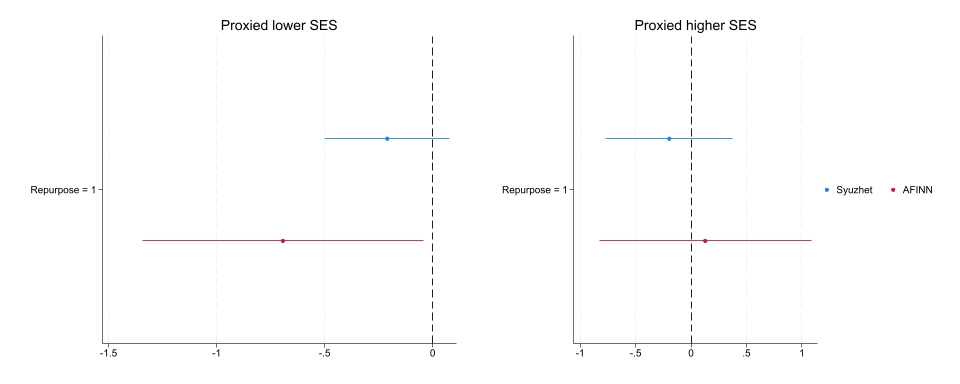
\includegraphics[width=17.6cm]{pictures_1/ses_het_sentiment.jpg} }}%
	
	\caption{Estimated effects of reusing practices on students' survey emotions in defining the mafia by proxied SES.
	}
	\label{fig:jmp_ses_sentiment}
	
\end{figure}

\emph{Household-level effect.} A final concern is that the cultural activities on the repurposed properties reshape the attitudes of the wider community rather than of students directly, and that the shift I document among students is a mediated reflection of their families' changing views. If so, the mechanism would operate at the household level, and attributing it to a change in students' own perceptions would be misleading.

I test this using a survey question asking students to report their family's opinion about the Mafia. If repurposing shifts attitudes at the household level, treated areas should show a change in the distribution of reported family opinions. Figure~\ref{fig:jmp_survey_career_families} reports the effect of reuse on the share of students attributing each stance to their family. The estimates are close to zero and statistically insignificant across every category: there is no detectable shift in how students describe their families' views of the Mafia following the intervention. The absence of any effect on reported family opinions indicates that the attitudinal change operates at the level of the students themselves rather than being transmitted through the household, consistent with a mechanism in which the repurposed property acts directly on juveniles through the alternative role models and community engagement it provides.

\begin{figure}[H]%
	\centering
	{{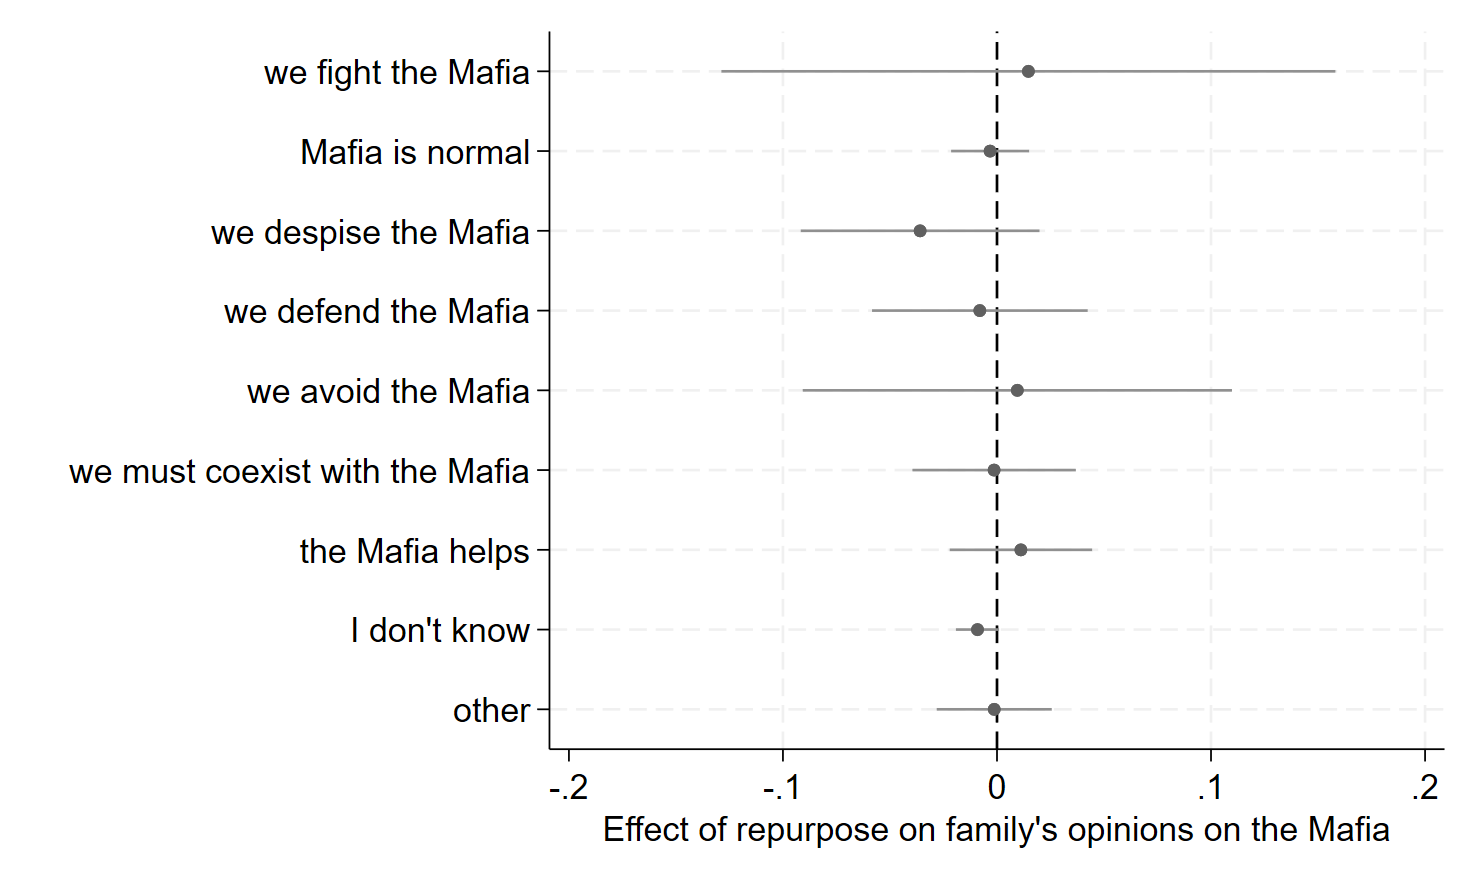
\includegraphics[width=15.4cm]{pictures_1/v21_coeffplot.png} }}%
	\caption{Estimated effects of repurposing practices on students' families' perception of the Mafia reported by students. Each point reports the effect of repurpose on the share of students agreeing with specific statements. Standard errors are clustered at the school level. Results are significant at the 90\% confidence level.
	}
	\label{fig:jmp_survey_career_families}
	%say that the new policy gave a new emotional wave on the reallocation in general
\end{figure}


\FloatBarrier
\section{Conclusions}
\label{sec:jmp_conclusions}

This study provides the first causal evidence that converting confiscating Mafia properties into community spaces yields tangible educational benefits for youth in historically Mafia-affected areas. I construct a comprehensive dataset tracking the implementation of the CRR policy across major urban areas, combining scraped records on confiscated assets, internal surveys from \emph{Libera}, municipal records, digitised Antimafia Investigative Directorate maps of baseline Mafia presence, Ministry of Education administrative records, and survey data on students' perceptions of the Mafia. I follow student cohorts from grade 9 to grade 13 and build school catchment areas by matching census blocks to their closest high school for each schooling track. Catchment areas are defined as treated whenever at least one Mafia property has been repurposed within their boundaries, and I compare treated areas to those unaffected or not yet affected, before and after the first repurposing event.

Using a difference-in-differences design, I find that transforming former criminal strongholds into hubs for social activities reduces high school dropout rates by approximately 36\% relative to baseline levels among students beyond the age of compulsory schooling. The effect emerges between two and three years after the first repurposing and persists for up to six years. Its magnitude scales with intensity: each additional repurposed property in a catchment area corresponds to a further reduction of roughly 12 per cent relative to the mean, and the effect is stronger where repurposed properties are closer to the student population-weighted centroid and where they are concentrated relative to the local student population.

The heterogeneity analysis reveals a consistent pattern. The effects are concentrated among students in low-performing schools and in technical high schools, the two groups facing the greatest structural barriers to completing their education, and are entirely driven by the repurposing of \emph{operational properties} rather than by commercial or industrial assets. Across activity types the point estimates are of broadly similar magnitude, differing in precision rather than in size. That the effect does not vary with what the property is used for, but does vary sharply with what the property once represented, points toward a channel operating through the visible reclaiming of the space rather than through the services delivered within it.

Survey evidence on students' perceptions supports this interpretation. Following repurposing, students are less likely to regard Mafia and political connections as useful routes to employment, and more likely to value education and civil-service examinations. This shift emerges around three years after treatment, on the same horizon at which dropout begins to decline. I also find evidence of a change in perceived State capacity: students become less likely to believe that the State does too little to confront the Mafia or that the Mafia infiltrates the State, and less likely to name the police and local politicians among the institutions they trust least. These responses appear within the first year of treatment and fade thereafter, suggesting that the initial signal of State presence operates upstream of the slower revision of beliefs about the returns to each pathway.

I rule out several alternative channels. The effect does not appear at the confiscation stage, when the controlling family is arrested and removed, which is difficult to reconcile with an incapacitation mechanism. It is not accompanied by any change in graduating grades, nor absorbed by concurrent municipal educational and social-inclusion programmes, as an educational-inputs channel would predict. Triple-difference estimates interacting the treatment with neighbourhood rental prices are close to zero, ruling out concurrent gentrification. Controlling for the presence of other NGOs in the catchment area leaves the estimate unchanged while the NGO variable itself is insignificant, indicating that the activities hosted in repurposed Mafia properties are not readily substitutable by conventional civil-society provision. Sentiment analysis of students' open-ended definitions of the Mafia shows a shift toward more negative language, in both frequency and intensity, and this shift is strongest among students producing the least linguistically complex responses — the group least equipped to reproduce a socially approved framing, which is difficult to reconcile with social desirability. Reported family attitudes show no change, locating the response with students themselves rather than with their households.

These findings carry implications for anti-Mafia policy design, in Italy and in comparable settings internationally. Most fundamentally, they show that effective prevention requires moving beyond asset confiscation toward the active construction of legitimate alternatives within affected communities. The binding constraint is not seizure but reuse: a substantial share of confiscated assets remain vacant or are never reassigned, and the evidence here indicates that seizure alone leaves little visible trace in the neighbourhood. The timing of the effects reinforces this. Because the behavioural response depends on sustained and visible use rather than on the announcement of reassignment, properties transferred and subsequently left inactive are unlikely to generate lasting benefits. Accelerating the transition from reallocation to active reuse, and providing sustained financial support to the local organisations that manage these spaces, would amplify the policy's reach. That the effects are largest among students in underperforming schools and from more disadvantaged backgrounds suggests the policy may operate as an equalising force, directing its benefits toward those with the fewest alternatives.

\setcounter{chapter}{1}
\newpage
\addcontentsline{toc}{section}{\textit{Appendices}}
\renewcommand{\thesection}{\Alph{section}}
\renewcommand{\thesubsection}{\thesection.\arabic{subsection}}
\renewcommand{\thefigure}{\Alph{section}.\arabic{figure}}
\renewcommand{\thetable}{\Alph{section}.\arabic{table}}
\setcounter{section}{0}
\setcounter{figure}{0}
\setcounter{table}{0}
\section{Additional Figures and Tables}
\label{sec:jmp_app_A}
  \begin{figure}[H]
  \begin{center}
    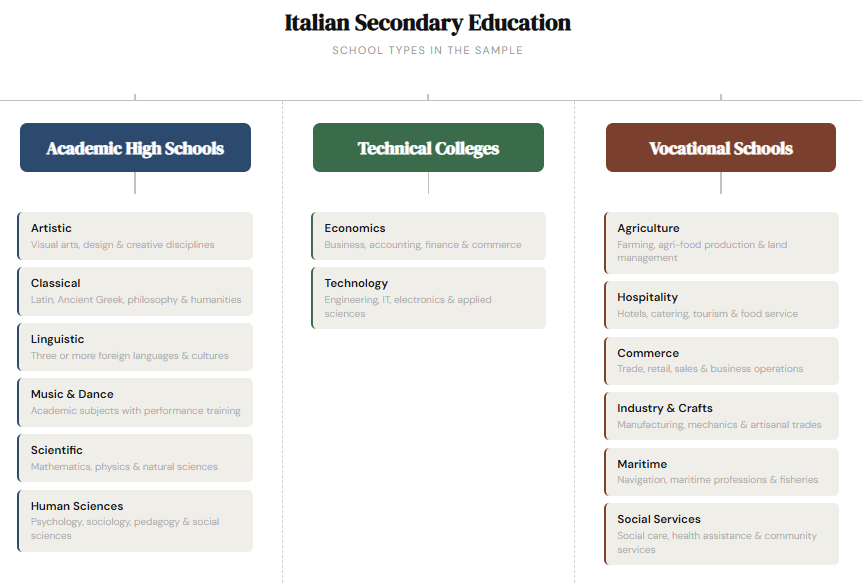
\includegraphics[scale=0.95]{pictures_1/school_type.png}
    \centering
    \caption{The universe of possible high school sub-tracks in Italy.}
      \label{fig:school_types}
    \end{center}
    \end{figure}

\begin{table}[H]
	\centering
	\caption{Survey questions from the Survey on the Perception of the Mafia}
	\label{tab:survey_questions}
	\small
	\begin{tabular}{@{}llp{0.42\textwidth}ll@{}}
		\toprule
		\textbf{ID} & \textbf{Topic} & \textbf{Question} & \textbf{Response} & \textbf{Unit} \\
		\midrule
		V12 & Definition & How would you define the Mafia? & Open-ended & Student \\
		V21 & Family view & How is the Mafia regarded within your family? & 9 options & School \\
		V28 & Job-seeking & In your town, what is most useful to do when looking for work? & 7 items, ranked 1--7 & School \\
		V33 & State vs.\ Mafia & Do you agree with each of the following statements? & 9 items, yes/no/don't know & School \\
		V45 & Trust & How much trust do you place in each of the following? & 10 items, scale 1--4 & School \\
		\bottomrule
		\multicolumn{5}{@{}p{1.1\textwidth}@{}}{\footnotesize Notes: Survey responses provided by \citet{centro_studi_pio_la_torre_survey_2025}. Full response items are listed in Appendix~\ref{sec:jmp_app_D}. Outcomes are school-level shares of students selecting each category; for V28 I use the top two (1--2) and bottom two (6--7) ranks. V12 is analysed at student level.} \\
	\end{tabular}
\end{table}

          \begin{figure}[H]
  \begin{center}
    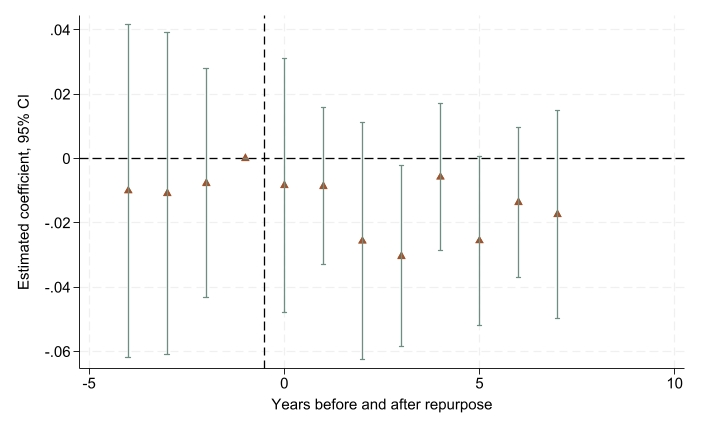
\includegraphics[scale=0.85]{pictures_1/main_exclg13_dropout.jpg}
    \centering
    \caption{Estimated effects of reusing practices on dropout rate before and after the first reuse
starts - excluding dropout from grade 13}
    \label{fig:es_excl_g13_}
    \end{center}
    \end{figure}
    
    
         \begin{figure}[H]
  \begin{center}
    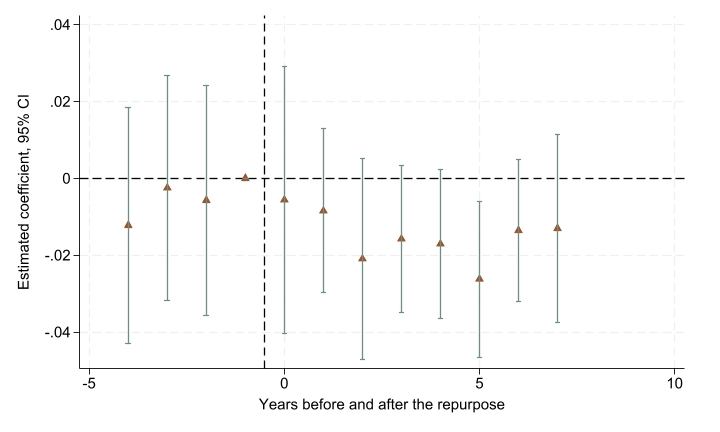
\includegraphics[scale=0.85]{pictures_1/evertreated_es.jpg}
    \centering

    \caption{Estimated effects of reusing practices on dropout rate before and after the first reuse
starts - event study of areas already hosting reallocated properties}
\label{fig:es_evertreated}
    \end{center}
    \end{figure}
    
    \begin{table}[H]
\caption{Testing the effect of the treatment on the main controls}
\label{tab:jmp_main_controls}
\vspace{0.2cm}
\centering
\scalebox{0.75}{
    \begin{tabular}{p{7.39em}llll}
    \toprule
    \multicolumn{1}{l}{} & \multicolumn{1}{c}{(1)} & \multicolumn{1}{c}{(2)} & \multicolumn{1}{c}{(3)} & \multicolumn{1}{c}{(4)} \\
    \multicolumn{1}{r}{} & \multicolumn{2}{c}{\textbf{Student migration}} & \multicolumn{2}{c}{\textbf{Grade retention}} \\
    \midrule
    \multicolumn{1}{l}{} & \multicolumn{1}{c}{} & \multicolumn{1}{c}{} & \multicolumn{1}{c}{} & \multicolumn{1}{c}{} \\
    \multicolumn{1}{l}{Reuse = 1} & \multicolumn{1}{c}{0.00160} & \multicolumn{1}{c}{0.00159} & \multicolumn{1}{c}{-0.000460} & \multicolumn{1}{c}{0.000469} \\
    \multicolumn{1}{l}{} & \multicolumn{1}{c}{(0.00182)} & \multicolumn{1}{c}{(0.00182)} & \multicolumn{1}{c}{(0.00120)} & \multicolumn{1}{c}{(0.00114)} \\
    \multicolumn{1}{l}{} & \multicolumn{1}{c}{} & \multicolumn{1}{c}{} & \multicolumn{1}{c}{} & \multicolumn{1}{c}{} \\
    \multicolumn{1}{l}{clustered SE} & \multicolumn{1}{c}{yes} & \multicolumn{1}{c}{yes} & \multicolumn{1}{c}{yes} & \multicolumn{1}{c}{yes} \\
    \multicolumn{1}{l}{School FE} & \multicolumn{1}{c}{yes} & \multicolumn{1}{c}{yes} & \multicolumn{1}{c}{yes} & \multicolumn{1}{c}{yes} \\
    \multicolumn{1}{l}{Time FE} & \multicolumn{1}{c}{yes} & \multicolumn{1}{c}{yes} & \multicolumn{1}{c}{yes} & \multicolumn{1}{c}{yes} \\
    \multicolumn{1}{l}{Student migration} & \multicolumn{1}{c}{no} & \multicolumn{1}{c}{no} & \multicolumn{1}{c}{no} & \multicolumn{1}{c}{yes} \\
    \multicolumn{1}{l}{Grade retention} & \multicolumn{1}{c}{no} & \multicolumn{1}{c}{yes} & \multicolumn{1}{c}{no} & \multicolumn{1}{c}{no} \\
    \multicolumn{1}{l}{Observations} & \multicolumn{1}{c}{1,294} & \multicolumn{1}{c}{1,292} & \multicolumn{1}{c}{1,542} & \multicolumn{1}{c}{1,292} \\
    \multicolumn{1}{l}{Number of schools} & \multicolumn{1}{c}{234} & \multicolumn{1}{c}{234} & \multicolumn{1}{c}{244} & \multicolumn{1}{c}{234} \\
    \multicolumn{1}{l}{Mean dep. var.} & \multicolumn{1}{c}{0.349} & \multicolumn{1}{c}{0.349} & \multicolumn{1}{c}{0.0108} & \multicolumn{1}{c}{0.0105} \\
    \midrule
    \multicolumn{5}{p{27.39em}}{Notes: TWFE model. The treatment variable is equal to 1 whenever there is at least one Mafia property within the school catchment area. Standard errors are clustered at the school level.} \\
    \end{tabular}%
}
\end{table}

    
\begin{table}[H]
\caption{Effect of the treatment on selection in enrollment preferences}
\label{tab:jmp_enrollment_selection}
\vspace{0.2cm}
\centering
\scalebox{0.75}{
    \begin{tabular}{p{16.835em}llll}
    \toprule
    \multicolumn{1}{l}{} & \multicolumn{1}{c}{(1)} & \multicolumn{1}{c}{(2)} & \multicolumn{1}{c}{(3)} & \multicolumn{1}{c}{(4)} \\
    \multicolumn{1}{r}{} & \multicolumn{4}{c}{Enrollment Share} \\
    \midrule
    \multicolumn{1}{l}{} & \multicolumn{1}{c}{} & \multicolumn{1}{c}{} & \multicolumn{1}{c}{} & \multicolumn{1}{c}{} \\
    \multicolumn{1}{l}{Reuse = 1 X Technical } & \multicolumn{1}{c}{-0.00723} & \multicolumn{1}{c}{-0.0117} & \multicolumn{1}{c}{-0.00778} & \multicolumn{1}{c}{-0.0116} \\
    \multicolumn{1}{l}{} & \multicolumn{1}{c}{(0.0127)} & \multicolumn{1}{c}{(0.0121)} & \multicolumn{1}{c}{(0.0125)} & \multicolumn{1}{c}{(0.0115)} \\
    \multicolumn{1}{l}{Reuse = 1 X Academic} & \multicolumn{1}{c}{0.0120} & \multicolumn{1}{c}{0.0240} & \multicolumn{1}{c}{0.0121} & \multicolumn{1}{c}{0.0235*} \\
    \multicolumn{1}{l}{} & \multicolumn{1}{c}{(0.0148)} & \multicolumn{1}{c}{(0.0145)} & \multicolumn{1}{c}{(0.0147)} & \multicolumn{1}{c}{(0.0140)} \\
    \multicolumn{1}{l}{Reuse = 1 X Vocational} & \multicolumn{1}{c}{-0.0638**} & \multicolumn{1}{c}{-0.0647**} & \multicolumn{1}{c}{-0.0637**} & \multicolumn{1}{c}{-0.0645**} \\
    \multicolumn{1}{l}{} & \multicolumn{1}{c}{(0.0250)} & \multicolumn{1}{c}{(0.0266)} & \multicolumn{1}{c}{(0.0246)} & \multicolumn{1}{c}{(0.0258)} \\
    \multicolumn{1}{l}{} & \multicolumn{1}{c}{} & \multicolumn{1}{c}{} & \multicolumn{1}{c}{} & \multicolumn{1}{c}{} \\
    \multicolumn{1}{l}{clustered SE} & \multicolumn{1}{c}{yes} & \multicolumn{1}{c}{yes} & \multicolumn{1}{c}{yes} & \multicolumn{1}{c}{yes} \\
    \multicolumn{1}{l}{school FE} & \multicolumn{1}{c}{yes} & \multicolumn{1}{c}{yes} & \multicolumn{1}{c}{yes} & \multicolumn{1}{c}{yes} \\
    \multicolumn{1}{l}{time FE} & \multicolumn{1}{c}{yes} & \multicolumn{1}{c}{yes} & \multicolumn{1}{c}{yes} & \multicolumn{1}{c}{yes} \\
    \multicolumn{1}{l}{migration} & \multicolumn{1}{c}{no} & \multicolumn{1}{c}{yes} & \multicolumn{1}{c}{no} & \multicolumn{1}{c}{yes} \\
    \multicolumn{1}{l}{retention} & \multicolumn{1}{c}{no} & \multicolumn{1}{c}{no} & \multicolumn{1}{c}{yes} & \multicolumn{1}{c}{yes} \\
    \multicolumn{1}{l}{Observations} & \multicolumn{1}{c}{1,496} & \multicolumn{1}{c}{1,254} & \multicolumn{1}{c}{1,471} & \multicolumn{1}{c}{1,235} \\
    \multicolumn{1}{l}{Number of schools} & \multicolumn{1}{c}{236} & \multicolumn{1}{c}{228} & \multicolumn{1}{c}{235} & \multicolumn{1}{c}{228} \\
    \multicolumn{1}{l}{Mean dep. var.} & \multicolumn{1}{c}{0.232} & \multicolumn{1}{c}{0.230} & \multicolumn{1}{c}{0.232} & \multicolumn{1}{c}{0.230} \\
    \midrule
    \multicolumn{5}{p{36.835em}}{Notes: TWFE model. The treatment variable is equal to 1 whenever there is at least one Mafia property within the school catchment area. Standard errors are clustered at the school level.} \\
    \end{tabular}%
    }
    \end{table}


      \begin{figure}[H]
  \begin{center}
    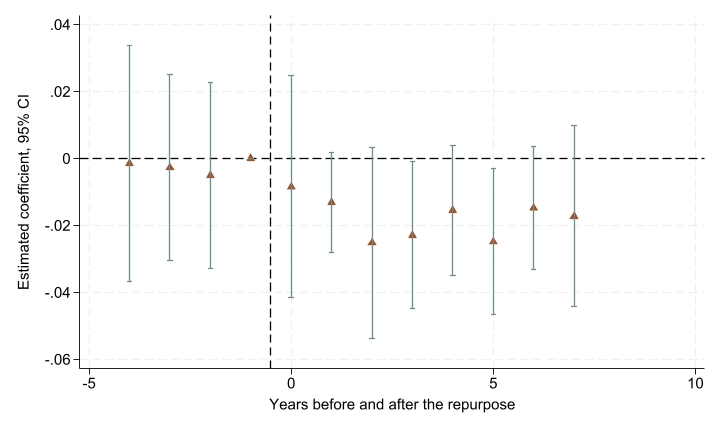
\includegraphics[scale=0.85]{pictures_1/alternativeexpl_es.jpg}
    \centering
    \caption{Estimated effects of reusing practices on dropout rate before and after the first reuse
starts - event study controlling for the presence of educational- and urban-related programmes at the municipality level}
    \label{fig:es_alt_expl}
    \end{center}
    \end{figure}

      \begin{figure}[H]
  \begin{center}
    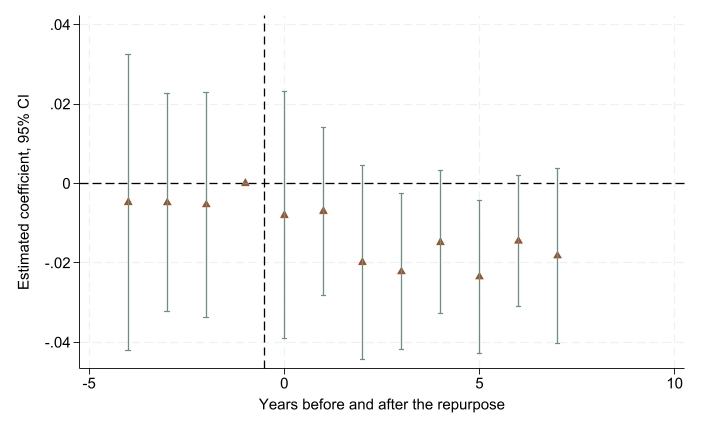
\includegraphics[scale=0.85]{pictures_1/alternativeexplngo_es.jpg}
    \centering
  
    \caption{Estimated effects of reusing practices on dropout rate before and after the first reuse
starts - event study controlling for the presence of NGOs}
\label{fig:es_alt_ngo}
    \end{center}
    \end{figure}

         \begin{figure}[H]
  \begin{center}
    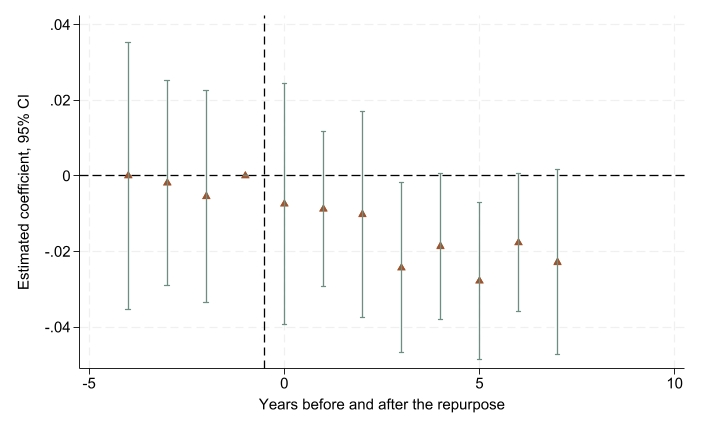
\includegraphics[scale=0.85]{pictures_1/reallocation_es.jpg}
    \centering
   
    \caption{Estimated effects of reusing practices on dropout rate before and after the first reuse
starts - event study of marginal effect over reallocations}
    \label{fig:es_reallocation}
    \end{center}
    \end{figure}
    
\begin{figure}[H]
  \begin{center}
    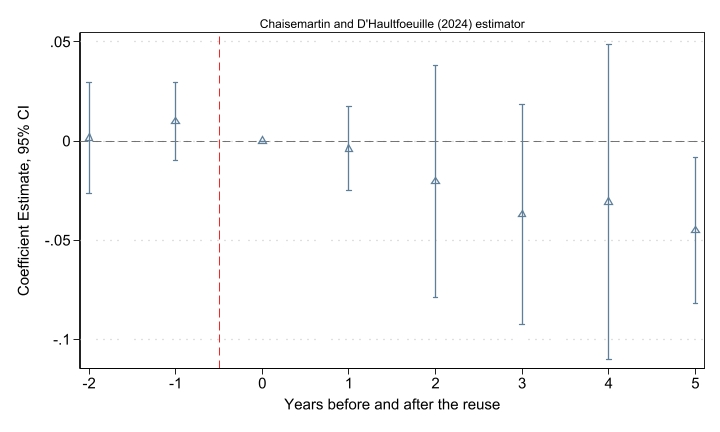
\includegraphics[scale=0.75]{pictures_1/cont_rob_stw.jpg}
    \centering\caption{Event study using the count of reused assets weighted by the student population of school catchment areas}
    \label{fig:jmp_es_stw}
    \end{center}
    \end{figure}

    \begin{figure}[H]
  \begin{center}
    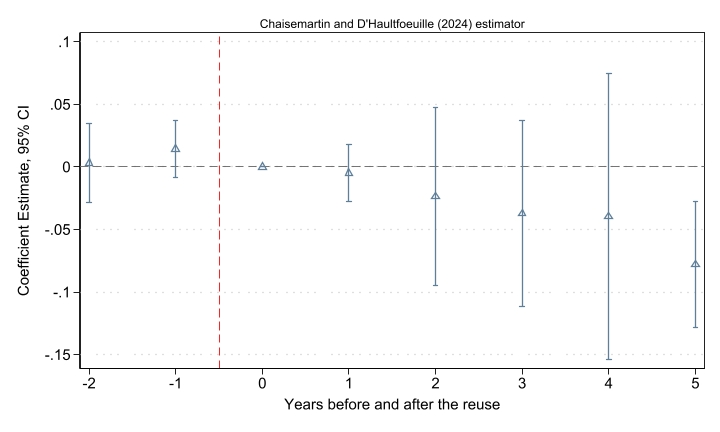
\includegraphics[scale=0.75]{pictures_1/cont_rob_dist.jpg}
    \centering\caption{Event study using the count of reused assets weighted by the average distance of properties from the population-weighted centroids of schools' catchment areas}
    \label{fig:jmp_es_dist}
    \end{center}
    \end{figure}


\begin{table}[H]
	\caption{Impact of reusing Mafia real estate on dropout rates for G11-G13} % Table label
	\label{tab:jmp_repurpose_types}
	\vspace{0.2cm}
	\centering
	\scalebox{0.85}{
		\begin{tabular}{p{12.39em}llll}
			\toprule
			\multicolumn{1}{l}{} & \multicolumn{1}{c}{(1)} & \multicolumn{1}{c}{(2)} & \multicolumn{1}{c}{(3)} & \multicolumn{1}{c}{(4)} \\
			\multicolumn{1}{c}{\textit{Types of repurpose}} & \multicolumn{4}{c}{\textbf{Dropout rate G11-G13}} \\
			\midrule
			\multicolumn{1}{l}{} & \multicolumn{1}{c}{} & \multicolumn{1}{c}{} & \multicolumn{1}{c}{} & \multicolumn{1}{c}{} \\
			\multicolumn{1}{l}{Education = 1} & \multicolumn{1}{c}{-0.0170} & \multicolumn{1}{c}{} & \multicolumn{1}{c}{} & \multicolumn{1}{c}{} \\
			\multicolumn{1}{l}{} & \multicolumn{1}{c}{(0.0114)} & \multicolumn{1}{c}{} & \multicolumn{1}{c}{} & \multicolumn{1}{c}{} \\
			\multicolumn{1}{l}{Education = 0} & \multicolumn{1}{c}{-0.0206*} & \multicolumn{1}{c}{} & \multicolumn{1}{c}{} & \multicolumn{1}{c}{} \\
			\multicolumn{1}{l}{} & \multicolumn{1}{c}{(0.0105)} & \multicolumn{1}{c}{} & \multicolumn{1}{c}{} & \multicolumn{1}{c}{} \\
			\multicolumn{1}{l}{Employment = 1} & \multicolumn{1}{c}{} & \multicolumn{1}{c}{-0.0141} & \multicolumn{1}{c}{} & \multicolumn{1}{c}{} \\
			\multicolumn{1}{l}{} & \multicolumn{1}{c}{} & \multicolumn{1}{c}{(0.0140)} & \multicolumn{1}{c}{} & \multicolumn{1}{c}{} \\
			\multicolumn{1}{l}{Employment = 0} & \multicolumn{1}{c}{} & \multicolumn{1}{c}{-0.0188**} & \multicolumn{1}{c}{} & \multicolumn{1}{c}{} \\
			\multicolumn{1}{l}{} & \multicolumn{1}{c}{} & \multicolumn{1}{c}{(0.00936)} & \multicolumn{1}{c}{} & \multicolumn{1}{c}{} \\
			\multicolumn{1}{l}{Culture = 1} & \multicolumn{1}{c}{} & \multicolumn{1}{c}{} & \multicolumn{1}{c}{-0.0162**} & \multicolumn{1}{c}{} \\
			\multicolumn{1}{l}{} & \multicolumn{1}{c}{} & \multicolumn{1}{c}{} & \multicolumn{1}{c}{(0.00767)} & \multicolumn{1}{c}{} \\
			\multicolumn{1}{l}{Culture = 0} & \multicolumn{1}{c}{} & \multicolumn{1}{c}{} & \multicolumn{1}{c}{-0.0222} & \multicolumn{1}{c}{} \\
			\multicolumn{1}{l}{} & \multicolumn{1}{c}{} & \multicolumn{1}{c}{} & \multicolumn{1}{c}{(0.0140)} & \multicolumn{1}{c}{} \\
			\multicolumn{1}{l}{Welfare = 1} & \multicolumn{1}{c}{} & \multicolumn{1}{c}{} & \multicolumn{1}{c}{} & \multicolumn{1}{c}{-0.0183*} \\
			\multicolumn{1}{l}{} & \multicolumn{1}{c}{} & \multicolumn{1}{c}{} & \multicolumn{1}{c}{} & \multicolumn{1}{c}{(0.00951)} \\
			\multicolumn{1}{l}{Welfare = 0} & \multicolumn{1}{c}{} & \multicolumn{1}{c}{} & \multicolumn{1}{c}{} & \multicolumn{1}{c}{-0.0252**} \\
			\multicolumn{1}{l}{} & \multicolumn{1}{c}{} & \multicolumn{1}{c}{} & \multicolumn{1}{c}{} & \multicolumn{1}{c}{(0.0114)} \\
			\multicolumn{1}{l}{} & \multicolumn{1}{c}{} & \multicolumn{1}{c}{} & \multicolumn{1}{c}{} & \multicolumn{1}{c}{} \\
			\multicolumn{1}{l}{clustered SE} & \multicolumn{1}{c}{yes} & \multicolumn{1}{c}{yes} & \multicolumn{1}{c}{yes} & \multicolumn{1}{c}{yes} \\
			\multicolumn{1}{l}{catchment school FE} & \multicolumn{1}{c}{yes} & \multicolumn{1}{c}{yes} & \multicolumn{1}{c}{yes} & \multicolumn{1}{c}{yes} \\
			\multicolumn{1}{l}{time FE} & \multicolumn{1}{c}{yes} & \multicolumn{1}{c}{yes} & \multicolumn{1}{c}{yes} & \multicolumn{1}{c}{yes} \\
			\multicolumn{1}{l}{migration} & \multicolumn{1}{c}{yes} & \multicolumn{1}{c}{yes} & \multicolumn{1}{c}{yes} & \multicolumn{1}{c}{yes} \\
			\multicolumn{1}{l}{retention} & \multicolumn{1}{c}{yes} & \multicolumn{1}{c}{yes} & \multicolumn{1}{c}{yes} & \multicolumn{1}{c}{yes} \\
			\multicolumn{1}{l}{Observations} & \multicolumn{1}{c}{1,274} & \multicolumn{1}{c}{1,274} & \multicolumn{1}{c}{1,274} & \multicolumn{1}{c}{1,274} \\
			\multicolumn{1}{l}{R-squared} & \multicolumn{1}{c}{0.091} & \multicolumn{1}{c}{0.091} & \multicolumn{1}{c}{0.091} & \multicolumn{1}{c}{0.091} \\
			\multicolumn{1}{l}{Number of codicescuolas} & \multicolumn{1}{c}{234} & \multicolumn{1}{c}{234} & \multicolumn{1}{c}{234} & \multicolumn{1}{c}{234} \\
			\multicolumn{1}{l}{Mean dep. var.} & \multicolumn{1}{c}{0.0530} & \multicolumn{1}{c}{0.0530} & \multicolumn{1}{c}{0.0530} & \multicolumn{1}{c}{0.0530} \\
			\midrule
			\multicolumn{5}{p{32.39em}}{Notes:} \\
		\end{tabular}%
	}
\end{table}
\FloatBarrier 

\begin{table}[H]
	\caption{Impact of reusing Mafia real estate on students’ perceptions on useful and useless channels to find a job in their town}
	\label{tab:jmp_v28}
	\vspace{0.2cm}
	\centering
	\scalebox{0.7}{
		    \begin{tabular}{p{12.39em}lllllll}
			\toprule
			\multicolumn{1}{l}{} & \multicolumn{1}{c}{(1)} & \multicolumn{1}{c}{(8)} & \multicolumn{1}{c}{(3)} & \multicolumn{1}{c}{(4)} & \multicolumn{1}{c}{(5)} & \multicolumn{1}{c}{(6)} & \multicolumn{1}{c}{(7)} \\
			\multicolumn{1}{l}{\textit{Dep. Variable}} & \multicolumn{1}{c}{Vocational training} & \multicolumn{1}{c}{Civil service} & \multicolumn{1}{c}{Ask the Mafia} & \multicolumn{1}{c}{Ask politician} & \multicolumn{1}{c}{Job centre} & \multicolumn{1}{c}{Ask family} & \multicolumn{1}{c}{Ask friend} \\
			\midrule
			\multicolumn{1}{l}{} & \multicolumn{1}{c}{} & \multicolumn{1}{c}{} & \multicolumn{1}{c}{} & \multicolumn{1}{c}{} & \multicolumn{1}{c}{} & \multicolumn{1}{c}{} & \multicolumn{1}{c}{} \\
			\multicolumn{1}{l}{\textit{\textbf{Panel A: more useful choices}}} &       &       &       &       &       &       &  \\
			\multicolumn{1}{l}{Repurpose = 1} & \multicolumn{1}{c}{0.161**} & \multicolumn{1}{c}{0.136} & \multicolumn{1}{c}{-0.110} & \multicolumn{1}{c}{-0.0754} & \multicolumn{1}{c}{0.0144} & \multicolumn{1}{c}{0.0371} & \multicolumn{1}{c}{0.0492} \\
			\multicolumn{1}{l}{} & \multicolumn{1}{c}{(0.0804)} & \multicolumn{1}{c}{(0.0827)} & \multicolumn{1}{c}{(0.0793)} & \multicolumn{1}{c}{(0.0863)} & \multicolumn{1}{c}{(0.0719)} & \multicolumn{1}{c}{(0.0405)} & \multicolumn{1}{c}{(0.0308)} \\
			\multicolumn{1}{l}{} & \multicolumn{1}{c}{} & \multicolumn{1}{c}{} & \multicolumn{1}{c}{} & \multicolumn{1}{c}{} & \multicolumn{1}{c}{} & \multicolumn{1}{c}{} & \multicolumn{1}{c}{} \\
			\multicolumn{1}{l}{Observations} & \multicolumn{1}{c}{161} & \multicolumn{1}{c}{161} & \multicolumn{1}{c}{161} & \multicolumn{1}{c}{161} & \multicolumn{1}{c}{161} & \multicolumn{1}{c}{161} & \multicolumn{1}{c}{161} \\
			\multicolumn{1}{l}{R-squared} & \multicolumn{1}{c}{0.400} & \multicolumn{1}{c}{0.548} & \multicolumn{1}{c}{0.425} & \multicolumn{1}{c}{0.484} & \multicolumn{1}{c}{0.472} & \multicolumn{1}{c}{0.443} & \multicolumn{1}{c}{0.562} \\
			\multicolumn{1}{l}{clustered SE} & \multicolumn{1}{c}{yes} & \multicolumn{1}{c}{yes} & \multicolumn{1}{c}{yes} & \multicolumn{1}{c}{yes} & \multicolumn{1}{c}{yes} & \multicolumn{1}{c}{yes} & \multicolumn{1}{c}{yes} \\
			\multicolumn{1}{l}{time FE} & \multicolumn{1}{c}{yes} & \multicolumn{1}{c}{yes} & \multicolumn{1}{c}{yes} & \multicolumn{1}{c}{yes} & \multicolumn{1}{c}{yes} & \multicolumn{1}{c}{yes} & \multicolumn{1}{c}{yes} \\
			\multicolumn{1}{l}{school FE} & \multicolumn{1}{c}{yes} & \multicolumn{1}{c}{yes} & \multicolumn{1}{c}{yes} & \multicolumn{1}{c}{yes} & \multicolumn{1}{c}{yes} & \multicolumn{1}{c}{yes} & \multicolumn{1}{c}{yes} \\
			\multicolumn{1}{l}{Mean dep. var.} & \multicolumn{1}{c}{0.480} & \multicolumn{1}{c}{0.426} & \multicolumn{1}{c}{0.280} & \multicolumn{1}{c}{0.280} & \multicolumn{1}{c}{0.400} & \multicolumn{1}{c}{0.303} & \multicolumn{1}{c}{0.273} \\
			\midrule
			\multicolumn{1}{r}{} &       &       &       &       &       &       &  \\
			\multicolumn{1}{l}{\textit{\textbf{Panel B: more useless choices}}} &       &       &       &       &       &       &  \\
			\multicolumn{1}{l}{Repurpose = 1} & \multicolumn{1}{c}{-0.0516} & \multicolumn{1}{c}{-0.0772} & \multicolumn{1}{c}{0.136*} & \multicolumn{1}{c}{0.117*} & \multicolumn{1}{c}{-0.00241} & \multicolumn{1}{c}{-0.0788} & \multicolumn{1}{c}{-0.0575} \\
			\multicolumn{1}{l}{} & \multicolumn{1}{c}{(0.0597)} & \multicolumn{1}{c}{(0.0469)} & \multicolumn{1}{c}{(0.0780)} & \multicolumn{1}{c}{(0.0662)} & \multicolumn{1}{c}{(0.0612)} & \multicolumn{1}{c}{(0.0614)} & \multicolumn{1}{c}{(0.0385)} \\
			\multicolumn{1}{r}{} &       &       &       &       &       &       &  \\
			\multicolumn{1}{l}{Observations} & \multicolumn{1}{c}{161} & \multicolumn{1}{c}{161} & \multicolumn{1}{c}{161} & \multicolumn{1}{c}{161} & \multicolumn{1}{c}{161} & \multicolumn{1}{c}{161} & \multicolumn{1}{c}{161} \\
			\multicolumn{1}{l}{R-squared} & \multicolumn{1}{c}{0.433} & \multicolumn{1}{c}{0.346} & \multicolumn{1}{c}{0.592} & \multicolumn{1}{c}{0.527} & \multicolumn{1}{c}{0.558} & \multicolumn{1}{c}{0.375} & \multicolumn{1}{c}{0.393} \\
			\multicolumn{1}{l}{clustered SE} & \multicolumn{1}{c}{yes} & \multicolumn{1}{c}{yes} & \multicolumn{1}{c}{yes} & \multicolumn{1}{c}{yes} & \multicolumn{1}{c}{yes} & \multicolumn{1}{c}{yes} & \multicolumn{1}{c}{yes} \\
			\multicolumn{1}{l}{time FE} & \multicolumn{1}{c}{yes} & \multicolumn{1}{c}{yes} & \multicolumn{1}{c}{yes} & \multicolumn{1}{c}{yes} & \multicolumn{1}{c}{yes} & \multicolumn{1}{c}{yes} & \multicolumn{1}{c}{yes} \\
			\multicolumn{1}{l}{school FE} & \multicolumn{1}{c}{yes} & \multicolumn{1}{c}{yes} & \multicolumn{1}{c}{yes} & \multicolumn{1}{c}{yes} & \multicolumn{1}{c}{yes} & \multicolumn{1}{c}{yes} & \multicolumn{1}{c}{yes} \\
			\multicolumn{1}{l}{Mean dep. var.} & \multicolumn{1}{c}{0.159} & \multicolumn{1}{c}{0.163} & \multicolumn{1}{c}{0.564} & \multicolumn{1}{c}{0.453} & \multicolumn{1}{c}{0.196} & \multicolumn{1}{c}{0.197} & \multicolumn{1}{c}{0.208} \\
			\midrule
			\multicolumn{8}{p{52.5em}}{Notes:} \\
		\end{tabular}%
		
	}
\end{table}



\begin{table}[H]
	\caption{Impact of reusing Mafia real estate on students’ perceptions of why people turn to the Mafia}
	\label{tab:jmp_v30}
	\vspace{0.2cm}
	\centering
	\scalebox{0.75}{
   \begin{tabular}{p{7.39em}llll}
   	\toprule
   	\multicolumn{1}{l}{} & \multicolumn{1}{c}{(1)} & \multicolumn{1}{c}{(2)} & \multicolumn{1}{c}{(3)} & \multicolumn{1}{c}{(4)} \\
   	\multicolumn{1}{l}{\textit{Dep. Variable}} & \multicolumn{1}{c}{Family ties} & \multicolumn{1}{c}{Neighbourhood} & \multicolumn{1}{c}{Lack of culture of legality} & \multicolumn{1}{c}{Looking for job} \\
   	\midrule
   	\multicolumn{1}{l}{} & \multicolumn{1}{c}{} & \multicolumn{1}{c}{} & \multicolumn{1}{c}{} & \multicolumn{1}{c}{} \\
   	\multicolumn{1}{l}{Repurpose = 1} & \multicolumn{1}{c}{0.0995***} & \multicolumn{1}{c}{0.0378} & \multicolumn{1}{c}{-0.0384} & \multicolumn{1}{c}{-0.0816***} \\
   	\multicolumn{1}{l}{} & \multicolumn{1}{c}{(0.0330)} & \multicolumn{1}{c}{(0.0391)} & \multicolumn{1}{c}{(0.0712)} & \multicolumn{1}{c}{(0.0278)} \\
   	\multicolumn{1}{l}{} & \multicolumn{1}{c}{} & \multicolumn{1}{c}{} & \multicolumn{1}{c}{} & \multicolumn{1}{c}{} \\
   	\multicolumn{1}{l}{Observations} & \multicolumn{1}{c}{161} & \multicolumn{1}{c}{161} & \multicolumn{1}{c}{161} & \multicolumn{1}{c}{161} \\
   	\multicolumn{1}{l}{R-squared} & \multicolumn{1}{c}{0.498} & \multicolumn{1}{c}{0.415} & \multicolumn{1}{c}{0.768} & \multicolumn{1}{c}{0.636} \\
   	\multicolumn{1}{l}{clustered SE} & \multicolumn{1}{c}{yes} & \multicolumn{1}{c}{yes} & \multicolumn{1}{c}{yes} & \multicolumn{1}{c}{yes} \\
   	\multicolumn{1}{l}{time FE} & \multicolumn{1}{c}{yes} & \multicolumn{1}{c}{yes} & \multicolumn{1}{c}{yes} & \multicolumn{1}{c}{yes} \\
   	\multicolumn{1}{l}{school FE} & \multicolumn{1}{c}{yes} & \multicolumn{1}{c}{yes} & \multicolumn{1}{c}{yes} & \multicolumn{1}{c}{yes} \\
   	\multicolumn{1}{l}{Mean dep. var.} & \multicolumn{1}{c}{0.160} & \multicolumn{1}{c}{0.109} & \multicolumn{1}{c}{0.206} & \multicolumn{1}{c}{0.130} \\
   	\midrule
   	\multicolumn{1}{r}{} &       &       &       &  \\
   	\midrule
   	\multicolumn{1}{l}{\textit{Dep. Variable}} & \multicolumn{1}{c}{Absent institutions} & \multicolumn{1}{c}{Looking for easy money} & \multicolumn{1}{c}{Looking for power} & \multicolumn{1}{c}{I don't know} \\
   	\multicolumn{1}{r}{} & \multicolumn{1}{c}{} & \multicolumn{1}{c}{} & \multicolumn{1}{c}{} & \multicolumn{1}{c}{} \\
   	\multicolumn{1}{l}{Repurpose = 1} & \multicolumn{1}{c}{-0.00753} & \multicolumn{1}{c}{0.107***} & \multicolumn{1}{c}{0.00948} & \multicolumn{1}{c}{-0.0112} \\
   	\multicolumn{1}{l}{} & \multicolumn{1}{c}{(0.0221)} & \multicolumn{1}{c}{(0.0375)} & \multicolumn{1}{c}{(0.0250)} & \multicolumn{1}{c}{(0.0141)} \\
   	\multicolumn{1}{l}{} & \multicolumn{1}{c}{} & \multicolumn{1}{c}{} & \multicolumn{1}{c}{} & \multicolumn{1}{c}{} \\
   	\multicolumn{1}{l}{Observations} & \multicolumn{1}{c}{161} & \multicolumn{1}{c}{138} & \multicolumn{1}{c}{138} & \multicolumn{1}{c}{161} \\
   	\multicolumn{1}{l}{R-squared} & \multicolumn{1}{c}{0.625} & \multicolumn{1}{c}{0.593} & \multicolumn{1}{c}{0.489} & \multicolumn{1}{c}{0.483} \\
   	\multicolumn{1}{l}{clustered SE} & \multicolumn{1}{c}{yes} & \multicolumn{1}{c}{yes} & \multicolumn{1}{c}{yes} & \multicolumn{1}{c}{yes} \\
   	\multicolumn{1}{l}{time FE} & \multicolumn{1}{c}{yes} & \multicolumn{1}{c}{yes} & \multicolumn{1}{c}{yes} & \multicolumn{1}{c}{yes} \\
   	\multicolumn{1}{l}{school FE} & \multicolumn{1}{c}{yes} & \multicolumn{1}{c}{yes} & \multicolumn{1}{c}{yes} & \multicolumn{1}{c}{yes} \\
   	\multicolumn{1}{l}{Mean dep. var.} & \multicolumn{1}{c}{0.0324} & \multicolumn{1}{c}{0.270} & \multicolumn{1}{c}{0.107} & \multicolumn{1}{c}{0.0401} \\
   	\midrule
   	Notes: &       &       &       &  \\
   \end{tabular}%
}
\end{table}

\begin{table}[H]
	\caption{Impact of reusing Mafia real estate on students’ perceptions of who is stronger between the Mafia and the State}
	\label{tab:jmp_v33}
	\vspace{0.2cm}
	\centering
	\scalebox{0.78}{
    \begin{tabular}{p{7.39em}lllll}
	\multicolumn{1}{r}{} &       &       &       &       &  \\
	\midrule
	\multicolumn{1}{l}{} & \multicolumn{1}{c}{(1)} & \multicolumn{1}{c}{(2)} & \multicolumn{1}{c}{(3)} & \multicolumn{1}{c}{(4)} & \multicolumn{1}{c}{(5)} \\
	\multicolumn{1}{l}{\textit{Dep. Variable}} & \multicolumn{1}{p{10em}}{State strong: we are the State} & \multicolumn{1}{p{9.78em}}{Mafia strong:infiltrates the State} & \multicolumn{1}{p{8.055em}}{Mafia strong: still exists} & \multicolumn{1}{p{8.665em}}{State strong: greater resources} & \multicolumn{1}{p{6.165em}}{State does too little} \\
	\midrule
	\multicolumn{1}{l}{} & \multicolumn{1}{c}{} & \multicolumn{1}{c}{} & \multicolumn{1}{c}{} & \multicolumn{1}{c}{} & \multicolumn{1}{c}{} \\
	\multicolumn{1}{l}{Repurpose =1  } & \multicolumn{1}{c}{0.322*} & \multicolumn{1}{c}{-0.109**} & \multicolumn{1}{c}{-0.132*} & \multicolumn{1}{c}{-0.111} & \multicolumn{1}{c}{-0.00382} \\
	\multicolumn{1}{l}{} & \multicolumn{1}{c}{(0.178)} & \multicolumn{1}{c}{(0.0447)} & \multicolumn{1}{c}{(0.0666)} & \multicolumn{1}{c}{(0.0859)} & \multicolumn{1}{c}{(0.101)} \\
	\multicolumn{1}{l}{} & \multicolumn{1}{c}{} & \multicolumn{1}{c}{} & \multicolumn{1}{c}{} & \multicolumn{1}{c}{} & \multicolumn{1}{c}{} \\
	\multicolumn{1}{l}{Observations} & \multicolumn{1}{c}{164} & \multicolumn{1}{c}{164} & \multicolumn{1}{c}{164} & \multicolumn{1}{c}{164} & \multicolumn{1}{c}{164} \\
	\multicolumn{1}{l}{R-squared} & \multicolumn{1}{c}{0.675} & \multicolumn{1}{c}{0.705} & \multicolumn{1}{c}{0.845} & \multicolumn{1}{c}{0.659} & \multicolumn{1}{c}{0.468} \\
	\multicolumn{1}{l}{clustered SE} & \multicolumn{1}{c}{yes} & \multicolumn{1}{c}{yes} & \multicolumn{1}{c}{yes} & \multicolumn{1}{c}{yes} & \multicolumn{1}{c}{yes} \\
	\multicolumn{1}{l}{time FE} & \multicolumn{1}{c}{yes} & \multicolumn{1}{c}{yes} & \multicolumn{1}{c}{yes} & \multicolumn{1}{c}{yes} & \multicolumn{1}{c}{yes} \\
	\multicolumn{1}{l}{school FE} & \multicolumn{1}{c}{yes} & \multicolumn{1}{c}{yes} & \multicolumn{1}{c}{yes} & \multicolumn{1}{c}{yes} & \multicolumn{1}{c}{yes} \\
	\multicolumn{1}{l}{Mean dep. var.} & \multicolumn{1}{c}{1.968} & \multicolumn{1}{c}{2.734} & \multicolumn{1}{c}{1.914} & \multicolumn{1}{c}{2.237} & \multicolumn{1}{c}{1.483} \\
	\midrule
	\multicolumn{1}{r}{} &       &       &       &       &  \\
	\cmidrule{2-6}    \multicolumn{1}{l}{\textit{Dep. Variable}} & \multicolumn{1}{p{10em}}{Mafia strong: any means to its ends} & \multicolumn{1}{p{9.78em}}{State strong: defends democracy} & \multicolumn{1}{p{8.055em}}{Mafia strong: instils fear} & \multicolumn{1}{p{8.665em}}{State and Mafia coincide} &  \\
	\cmidrule{2-6}    \multicolumn{1}{r}{} &       &       &       &       &  \\
	\multicolumn{1}{l}{Repurpose =1  } & \multicolumn{1}{c}{-0.0990} & \multicolumn{1}{c}{0.0792} & \multicolumn{1}{c}{-0.0951} & \multicolumn{1}{c}{-0.0872} &  \\
	\multicolumn{1}{r}{} & \multicolumn{1}{c}{(0.0711)} & \multicolumn{1}{c}{(0.163)} & \multicolumn{1}{c}{(0.127)} & \multicolumn{1}{c}{(0.0818)} &  \\
	\multicolumn{1}{r}{} &       &       &       &       &  \\
	\multicolumn{1}{l}{Observations} & \multicolumn{1}{c}{164} & \multicolumn{1}{c}{164} & \multicolumn{1}{c}{164} & \multicolumn{1}{c}{164} &  \\
	\multicolumn{1}{l}{R-squared} & \multicolumn{1}{c}{0.509} & \multicolumn{1}{c}{0.708} & \multicolumn{1}{c}{0.656} & \multicolumn{1}{c}{0.802} &  \\
	\multicolumn{1}{l}{clustered SE} & \multicolumn{1}{c}{yes} & \multicolumn{1}{c}{yes} & \multicolumn{1}{c}{yes} & \multicolumn{1}{c}{yes} &  \\
	\multicolumn{1}{l}{time FE} & \multicolumn{1}{c}{yes} & \multicolumn{1}{c}{yes} & \multicolumn{1}{c}{yes} & \multicolumn{1}{c}{yes} &  \\
	\multicolumn{1}{l}{school FE} & \multicolumn{1}{c}{yes} & \multicolumn{1}{c}{yes} & \multicolumn{1}{c}{yes} & \multicolumn{1}{c}{yes} &  \\
	\multicolumn{1}{l}{Mean dep. var.} & \multicolumn{1}{c}{2.741} & \multicolumn{1}{c}{1.752} & \multicolumn{1}{c}{2.387} & \multicolumn{1}{c}{2.117} &  \\
	\midrule
	\multicolumn{6}{p{50.055em}}{Notes:} \\
\end{tabular}%
}
\end{table}


\begin{table}[H]
	\caption{Impact of reusing Mafia real estate on students’ perceptions of who they can trust more}
	\label{tab:jmp_mafia_state}
	\vspace{0.2cm}
	\centering
	\scalebox{0.7}{
    \begin{tabular}{p{9.89em}llllllll}
	\toprule
	\multicolumn{1}{l}{} & \multicolumn{1}{c}{(1)} & \multicolumn{1}{c}{(2)} & \multicolumn{1}{c}{(3)} & \multicolumn{1}{c}{(4)} & \multicolumn{1}{c}{(5)} & \multicolumn{1}{c}{(6)} & \multicolumn{1}{c}{(7)} & \multicolumn{1}{c}{(8)} \\
	\multicolumn{1}{l}{\textit{Dep. Variable}} & \multicolumn{1}{c}{Magistrates} & \multicolumn{1}{c}{Police} & \multicolumn{1}{c}{Teachers} & \multicolumn{1}{c}{Journalists} & \multicolumn{1}{c}{Bankers} & \multicolumn{1}{c}{Priests} & \multicolumn{1}{c}{Local politicians} & \multicolumn{1}{c}{Trade unionists} \\
	\midrule
	\multicolumn{1}{l}{} & \multicolumn{1}{c}{} & \multicolumn{1}{c}{} & \multicolumn{1}{c}{} & \multicolumn{1}{c}{} & \multicolumn{1}{c}{} & \multicolumn{1}{c}{} & \multicolumn{1}{c}{} & \multicolumn{1}{c}{} \\
	\multicolumn{1}{l}{\textbf{Panel A: most trusted}} &       &       &       &       &       &       &       &  \\
	\multicolumn{1}{l}{Repurpose = 1} & \multicolumn{1}{c}{0.123} & \multicolumn{1}{c}{0.0107} & \multicolumn{1}{c}{-0.0160} & \multicolumn{1}{c}{-0.0548} & \multicolumn{1}{c}{-0.0267} & \multicolumn{1}{c}{0.0221} & \multicolumn{1}{c}{0.00150} & \multicolumn{1}{c}{0.0285} \\
	\multicolumn{1}{l}{} & \multicolumn{1}{c}{(0.113)} & \multicolumn{1}{c}{(0.0212)} & \multicolumn{1}{c}{(0.127)} & \multicolumn{1}{c}{(0.0496)} & \multicolumn{1}{c}{(0.0512)} & \multicolumn{1}{c}{(0.0376)} & \multicolumn{1}{c}{(0.0166)} & \multicolumn{1}{c}{(0.0610)} \\
	\multicolumn{1}{l}{} & \multicolumn{1}{c}{} & \multicolumn{1}{c}{} & \multicolumn{1}{c}{} & \multicolumn{1}{c}{} & \multicolumn{1}{c}{} & \multicolumn{1}{c}{} & \multicolumn{1}{c}{} & \multicolumn{1}{c}{} \\
	\multicolumn{1}{l}{Observations} & \multicolumn{1}{c}{164} & \multicolumn{1}{c}{164} & \multicolumn{1}{c}{164} & \multicolumn{1}{c}{164} & \multicolumn{1}{c}{164} & \multicolumn{1}{c}{164} & \multicolumn{1}{c}{164} & \multicolumn{1}{c}{164} \\
	\multicolumn{1}{l}{R-squared} & \multicolumn{1}{c}{0.780} & \multicolumn{1}{c}{0.689} & \multicolumn{1}{c}{0.693} & \multicolumn{1}{c}{0.597} & \multicolumn{1}{c}{0.663} & \multicolumn{1}{c}{0.681} & \multicolumn{1}{c}{0.559} & \multicolumn{1}{c}{0.528} \\
	\multicolumn{1}{l}{clustered SE} & \multicolumn{1}{c}{yes} & \multicolumn{1}{c}{yes} & \multicolumn{1}{c}{yes} & \multicolumn{1}{c}{yes} & \multicolumn{1}{c}{yes} & \multicolumn{1}{c}{yes} & \multicolumn{1}{c}{yes} & \multicolumn{1}{c}{yes} \\
	\multicolumn{1}{l}{time FE} & \multicolumn{1}{c}{yes} & \multicolumn{1}{c}{yes} & \multicolumn{1}{c}{yes} & \multicolumn{1}{c}{yes} & \multicolumn{1}{c}{yes} & \multicolumn{1}{c}{yes} & \multicolumn{1}{c}{yes} & \multicolumn{1}{c}{yes} \\
	\multicolumn{1}{l}{school FE} & \multicolumn{1}{c}{yes} & \multicolumn{1}{c}{yes} & \multicolumn{1}{c}{yes} & \multicolumn{1}{c}{yes} & \multicolumn{1}{c}{yes} & \multicolumn{1}{c}{yes} & \multicolumn{1}{c}{yes} & \multicolumn{1}{c}{yes} \\
	\multicolumn{1}{l}{Mean dep. var.} & \multicolumn{1}{c}{0.273} & \multicolumn{1}{c}{0.0402} & \multicolumn{1}{c}{0.377} & \multicolumn{1}{c}{0.114} & \multicolumn{1}{c}{0.0724} & \multicolumn{1}{c}{0.129} & \multicolumn{1}{c}{0.0277} & \multicolumn{1}{c}{0.253} \\
	\midrule
	\multicolumn{1}{r}{} &       &       &       &       &       &       &       &  \\
	\multicolumn{1}{l}{\textbf{Panel B: least trusted}} &       &       &       &       &       &       &       &  \\
	\multicolumn{1}{l}{Repurpose = 1} & \multicolumn{1}{c}{0.00747} & \multicolumn{1}{c}{-0.123*} & \multicolumn{1}{c}{0.00194} & \multicolumn{1}{c}{-0.0153} & \multicolumn{1}{c}{0.00380} & \multicolumn{1}{c}{0.0237} & \multicolumn{1}{c}{-0.167***} & \multicolumn{1}{c}{-0.0207} \\
	\multicolumn{1}{l}{} & \multicolumn{1}{c}{(0.0355)} & \multicolumn{1}{c}{(0.0727)} & \multicolumn{1}{c}{(0.0326)} & \multicolumn{1}{c}{(0.0361)} & \multicolumn{1}{c}{(0.0542)} & \multicolumn{1}{c}{(0.0584)} & \multicolumn{1}{c}{(0.0476)} & \multicolumn{1}{c}{(0.0537)} \\
	\multicolumn{1}{r}{} &       &       &       &       &       &       &       &  \\
	\multicolumn{1}{l}{Observations} & \multicolumn{1}{c}{164} & \multicolumn{1}{c}{164} & \multicolumn{1}{c}{164} & \multicolumn{1}{c}{164} & \multicolumn{1}{c}{164} & \multicolumn{1}{c}{164} & \multicolumn{1}{c}{164} & \multicolumn{1}{c}{164} \\
	\multicolumn{1}{l}{R-squared} & \multicolumn{1}{c}{0.819} & \multicolumn{1}{c}{0.892} & \multicolumn{1}{c}{0.715} & \multicolumn{1}{c}{0.816} & \multicolumn{1}{c}{0.761} & \multicolumn{1}{c}{0.422} & \multicolumn{1}{c}{0.826} & \multicolumn{1}{c}{0.506} \\
	\multicolumn{1}{l}{clustered SE} & \multicolumn{1}{c}{yes} & \multicolumn{1}{c}{yes} & \multicolumn{1}{c}{yes} & \multicolumn{1}{c}{yes} & \multicolumn{1}{c}{yes} & \multicolumn{1}{c}{yes} & \multicolumn{1}{c}{yes} & \multicolumn{1}{c}{yes} \\
	\multicolumn{1}{l}{time FE} & \multicolumn{1}{c}{yes} & \multicolumn{1}{c}{yes} & \multicolumn{1}{c}{yes} & \multicolumn{1}{c}{yes} & \multicolumn{1}{c}{yes} & \multicolumn{1}{c}{yes} & \multicolumn{1}{c}{yes} & \multicolumn{1}{c}{yes} \\
	\multicolumn{1}{l}{school FE} & \multicolumn{1}{c}{yes} & \multicolumn{1}{c}{yes} & \multicolumn{1}{c}{yes} & \multicolumn{1}{c}{yes} & \multicolumn{1}{c}{yes} & \multicolumn{1}{c}{yes} & \multicolumn{1}{c}{yes} & \multicolumn{1}{c}{yes} \\
	\multicolumn{1}{l}{Mean dep. var.} & \multicolumn{1}{c}{0.0946} & \multicolumn{1}{c}{0.405} & \multicolumn{1}{c}{0.0345} & \multicolumn{1}{c}{0.0928} & \multicolumn{1}{c}{0.122} & \multicolumn{1}{c}{0.213} & \multicolumn{1}{c}{0.390} & \multicolumn{1}{c}{0.0698} \\
	\midrule
	\multicolumn{9}{p{46.555em}}{Notes:} \\
\end{tabular}%
}
\end{table}


    
\begin{figure}[H]
  \begin{center}
    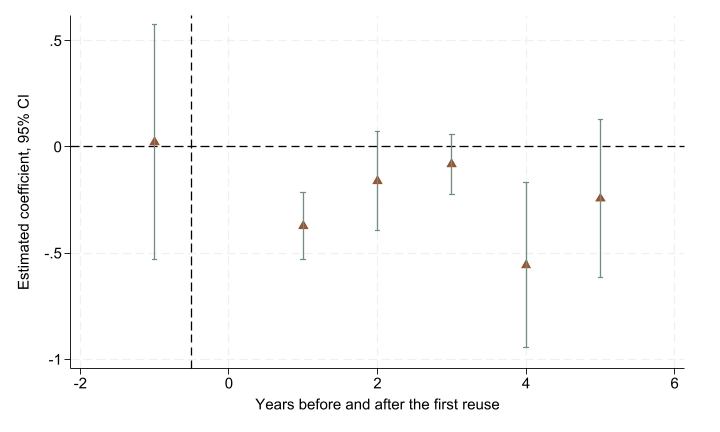
\includegraphics[scale=0.75]{pictures_1/syuzh_event.jpg}
    \centering\caption{Event study of the Szyuzhet scores}
    \label{fig:jmp_es_syuzhet}
    \end{center}
    \end{figure}

    \begin{figure}[H]
  \begin{center}
    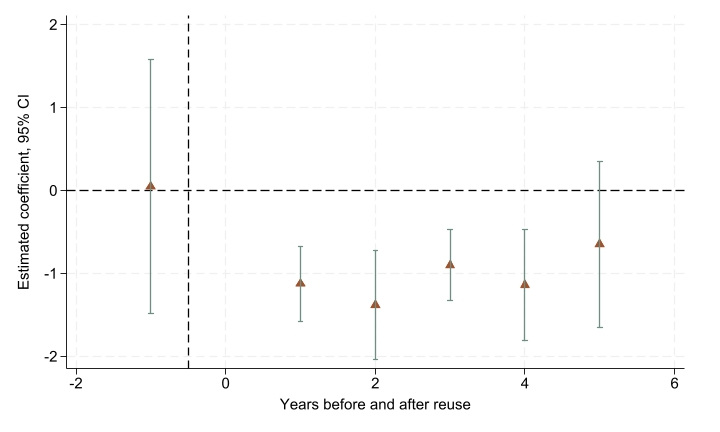
\includegraphics[scale=0.75]{pictures_1/sent_afinn.jpg}
    \centering\caption{Event study of the AFINN sentiment scores}
    \label{fig:jmp_es_afinn}
    \end{center}
    \end{figure}
    

\begin{table}[H]
\caption{Top 25\ terms for positive and negative sentiments} % Table label
\label{tab:jmp_nrc_terms}
\vspace{0.2cm}
\centering
\scalebox{0.68}{
    \begin{tabular}{p{14.055em}llll}
    \toprule
    \multicolumn{1}{l}{\textit{Panel A: top 25\% negative words}} & \multicolumn{1}{c}{\textbf{Anger}} & \multicolumn{1}{c}{\textbf{Disgust}} & \multicolumn{1}{c}{\textbf{Fear}} & \multicolumn{1}{c}{\textbf{Sadness}} \\
    \midrule
    \multicolumn{1}{r}{} & \multicolumn{1}{c}{Electoral } & \multicolumn{1}{c}{Ruthless} & \multicolumn{1}{c}{Forced} & \multicolumn{1}{c}{Violence} \\
    \multicolumn{1}{r}{} & \multicolumn{1}{c}{Laundering} & \multicolumn{1}{c}{Struggle} & \multicolumn{1}{c}{Eradicate} & \multicolumn{1}{c}{Kill} \\
    \multicolumn{1}{r}{} & \multicolumn{1}{c}{Murder} & \multicolumn{1}{c}{Threathening} & \multicolumn{1}{c}{Hide} & \multicolumn{1}{c}{Cruel} \\
    \multicolumn{1}{r}{} & \multicolumn{1}{c}{Resorting} & \multicolumn{1}{c}{Inconvenient} & \multicolumn{1}{c}{Manifests} & \multicolumn{1}{c}{Unfair} \\
    \multicolumn{1}{r}{} & \multicolumn{1}{c}{Conflict} & \multicolumn{1}{c}{Involve} & \multicolumn{1}{c}{Struggle} & \multicolumn{1}{c}{Evil} \\
    \multicolumn{1}{r}{} &       &       &       &  \\
    \multicolumn{1}{l}{Observations} & \multicolumn{1}{c}{638} & \multicolumn{1}{c}{393} & \multicolumn{1}{c}{327} & \multicolumn{1}{c}{274} \\
    \multicolumn{1}{r}{} &       &       &       &  \\
    \midrule
    \multicolumn{1}{l}{\textit{Panel B: top 25\% positive words}} & \multicolumn{1}{c}{\textbf{Joy}} & \multicolumn{1}{c}{\textbf{Trust}} & \multicolumn{1}{c}{\textbf{Surprise}} & \multicolumn{1}{c}{\textbf{Anticipation}} \\
    \midrule
    \multicolumn{1}{r}{} & \multicolumn{1}{c}{Money} & \multicolumn{1}{c}{Money} & \multicolumn{1}{c}{Money} & \multicolumn{1}{c}{Public} \\
    \multicolumn{1}{r}{} & \multicolumn{1}{c}{Respect} & \multicolumn{1}{c}{Association} & \multicolumn{1}{c}{Violent} & \multicolumn{1}{c}{Respect} \\
    \multicolumn{1}{r}{} & \multicolumn{1}{c}{Achieve} & \multicolumn{1}{c}{Structure} & \multicolumn{1}{c}{Protection} & \multicolumn{1}{c}{Protection} \\
    \multicolumn{1}{r}{} & \multicolumn{1}{c}{Gain} & \multicolumn{1}{c}{Respect} & \multicolumn{1}{c}{Deal } & \multicolumn{1}{c}{Gain} \\
    \multicolumn{1}{r}{} & \multicolumn{1}{c}{Freedom} & \multicolumn{1}{c}{Achieve} & \multicolumn{1}{c}{Hope} & \multicolumn{1}{c}{Poweful} \\
    \multicolumn{1}{r}{} &       &       &       &  \\
    \multicolumn{1}{l}{Observations} & \multicolumn{1}{c}{227} & \multicolumn{1}{c}{569} & \multicolumn{1}{c}{740} & \multicolumn{1}{c}{234} \\
    \midrule
    \multicolumn{5}{p{41.555em}}{Those words you listed are the most frequent words appearing in sentences that scored high (top 25\%) for each specific emotion dummy.} \\
    \end{tabular}%
    }
    \end{table}

    

\begin{table}[H]
\caption{Examples of students' definitions of the Mafia} % Table label
\label{tab:jmp_ses_rank}
\vspace{0.2cm}
\centering
\scalebox{0.78}{
    \begin{tabular}{p{5.39em}lll}
    \multicolumn{1}{c}{Rank} & \multicolumn{1}{p{19em}}{Definition} & \multicolumn{1}{c}{Italian word count} & \multicolumn{1}{c}{CSI} \\
    \midrule
    \multicolumn{1}{c}{0} & \multicolumn{1}{p{19em}}{I don't know} & \multicolumn{1}{c}{2} & \multicolumn{1}{c}{-0.35} \\
    \multicolumn{1}{c}{1} & \multicolumn{1}{p{19em}}{They are organizations that ruin our society} & \multicolumn{1}{c}{7} & \multicolumn{1}{c}{-0.22} \\
    \multicolumn{1}{c}{2} & \multicolumn{1}{p{19em}}{Organizations that follow, therefore adopt, a behavior that may seem beneficial in some aspects such as the economic one and employment} & \multicolumn{1}{c}{21} & \multicolumn{1}{c}{0.12} \\
    \multicolumn{1}{c}{3} & \multicolumn{1}{p{19em}}{Mafia-type organizations are a group of people who act illegally, sometimes hiding behind legal activities. Very often mafia organizations push people towards the wrong path, very often due to people's desperation} & \multicolumn{1}{c}{40} & \multicolumn{1}{c}{0.59} \\
    \midrule
    \multicolumn{4}{p{39.445em}}{} \\
    \end{tabular}%
    }
    \end{table}

\newpage
\renewcommand{\thefigure}{B.\arabic{figure}}
\renewcommand{\thetable}{B.\arabic{table}}
\setcounter{figure}{0}
\setcounter{table}{0}
\FloatBarrier
\section{Attributes of repurposed properties and local context}
\label{sec:jmp_app_B}
The repurposed properties in the sample display a fairly homogeneous profile in terms of real estate type. The large majority are residential estates (68\%), followed by land (20\%), while commercial and industrial properties account for only 10\% and a residual share falls into other categories. Consistent with this, the most common prior use before confiscation was villas and houses (45\%), followed by other uses (26\%) and land (19\%), with shops, garages, and commercial deposits representing marginal shares. In terms of reallocation, virtually all properties (99\%) were transferred to local authorities, with only one asset sold to a private buyer. Regarding the activities carried out in the repurposed properties, the distribution is relatively balanced between welfare and cultural activities — roughly half of the properties host welfare-oriented activities (50.6\%) and a slightly larger share host cultural ones (56.4\%) — while employment and other activities remain much less common, at 11.6\% and 12.1\% respectively. Education activities are present in about one fifth of cases (19.4\%).
\begin{table}[H]
\centering
\caption{Repurposed properties attributes}
\label{tab:property_attributes}
\scalebox{0.85}{
    \begin{tabular}{p{14.89em}llllll}
    \multicolumn{1}{l}{\textbf{Type of real estate}} & \multicolumn{1}{c}{N} & \multicolumn{1}{c}{\%} &       & \textbf{Reallocation type} & \multicolumn{1}{c}{N} & \multicolumn{1}{c}{\%} \\
    \midrule
    \multicolumn{1}{l}{Commercial and industrial estate} & \multicolumn{1}{c}{35} & \multicolumn{1}{c}{10} &       & Local authorities & \multicolumn{1}{c}{345} & \multicolumn{1}{c}{99} \\
    \multicolumn{1}{l}{Residential estate} & \multicolumn{1}{c}{236} & \multicolumn{1}{c}{68} &       & Sold to private & \multicolumn{1}{c}{1} & \multicolumn{1}{c}{1} \\
    \multicolumn{1}{l}{Land} & \multicolumn{1}{c}{67} & \multicolumn{1}{c}{20} &       & Total & \multicolumn{1}{c}{346} & \multicolumn{1}{c}{100} \\
    \multicolumn{1}{l}{Other} & \multicolumn{1}{c}{8} & \multicolumn{1}{c}{2} &       &       &       &  \\
    \multicolumn{1}{l}{Total} & \multicolumn{1}{c}{346} & \multicolumn{1}{c}{100} &       &       &       &  \\
    \multicolumn{1}{c}{} &       &       &       &       &       &  \\
    \multicolumn{1}{l}{\textbf{Usage before confiscation}} & \multicolumn{1}{c}{N} & \multicolumn{1}{c}{\%} &       & \textbf{All types of activities} & \multicolumn{1}{c}{N} & \multicolumn{1}{c}{\%} \\
        \midrule
    \multicolumn{1}{l}{Other} & \multicolumn{1}{c}{92} & \multicolumn{1}{c}{26} &       & Education & \multicolumn{1}{c}{67} & \multicolumn{1}{c}{19.4} \\
    \multicolumn{1}{l}{Box, garage} & \multicolumn{1}{c}{18} & \multicolumn{1}{c}{5} &       & Welfare & \multicolumn{1}{c}{175} & \multicolumn{1}{c}{50.6} \\
    \multicolumn{1}{l}{Fabbricate} & \multicolumn{1}{c}{3} & \multicolumn{1}{c}{1} &       & Culture & \multicolumn{1}{c}{195} & \multicolumn{1}{c}{56.4} \\
    \multicolumn{1}{l}{Commercial deposit} & \multicolumn{1}{c}{3} & \multicolumn{1}{c}{1} &       & Employment & \multicolumn{1}{c}{40} & \multicolumn{1}{c}{11.6} \\
    \multicolumn{1}{l}{Shop} & \multicolumn{1}{c}{11} & \multicolumn{1}{c}{3} &       & Other & \multicolumn{1}{c}{42} & \multicolumn{1}{c}{12.1} \\
    \multicolumn{1}{l}{Land} & \multicolumn{1}{c}{65} & \multicolumn{1}{c}{19} &       &       &       &  \\
    \multicolumn{1}{l}{Villas and Houses} & \multicolumn{1}{c}{155} & \multicolumn{1}{c}{45} &       &       &       &  \\
    \multicolumn{1}{l}{Total} & \multicolumn{1}{c}{346} & \multicolumn{1}{c}{100} &       &       &       &  \\
    \multicolumn{1}{c}{} &       &       &       &       &       &  \\
    \midrule
    \multicolumn{7}{p{36.44em}}{} \\
    \end{tabular}%
       }
    \end{table}

Turning to the local context, the data paint a picture of small, tight-knit, predominantly native residential communities. With an average of just 361 residents and 136 households per census section, these are not urban neighbourhoods in any dense sense — they are closer to village-scale settlements or peripheral urban pockets, the kind of places where social dynamics are likely shaped by proximity and long-standing local ties rather than anonymity. The very low share of non-native residents (under 4\% on average) reinforces this characterisation of socially homogeneous, relatively closed communities. Household composition skews toward smaller units, with single- and two-person households together accounting for over half the average section, which may reflect an ageing population rather than a young or dynamic one. Educational attainment is modest: high school and secondary diplomas dominate, university graduates make up only 13\% of residents, and a non-trivial share holds only a primary diploma or is merely literate. This suggests these are working- and lower-middle-class communities, not areas of high human capital concentration. Labour market conditions are consistent with this reading — while the employment rate averages around 77\%, unemployment sits at roughly 11\%, pointing to communities that are economically functional but under strain, without the slack of prosperous areas. The local real estate stock is overwhelmingly residential (81\%), mostly in good or decent physical condition, with a limited commercial footprint (15\%), further reinforcing the image of settled, predominantly domestic environments rather than economically active or commercially vibrant ones. Civic infrastructure is present but uneven: the average of 43 registered NGOs per area suggests some organised social fabric, but participation levels vary enormously across locations, indicating that civil society engagement is far from uniform and likely concentrated in a subset of better-resourced communities.
\begin{table}[H]
\centering
\caption{Census data}
\label{tab:census_data}
\scalebox{0.75}{

        \begin{tabular}{p{12.835em}lllll}
    \toprule
    \multicolumn{1}{l}{} & \multicolumn{1}{c}{(1)} & \multicolumn{1}{c}{(2)} & \multicolumn{1}{c}{(3)} & \multicolumn{1}{c}{(4)} & \multicolumn{1}{c}{(5)} \\
    \multicolumn{1}{r}{} & \multicolumn{1}{c}{N} & \multicolumn{1}{c}{mean} & \multicolumn{1}{c}{sd} & \multicolumn{1}{c}{min} & \multicolumn{1}{c}{max} \\
    \midrule
    \multicolumn{1}{l}{} & \multicolumn{1}{c}{} & \multicolumn{1}{c}{} & \multicolumn{1}{c}{} & \multicolumn{1}{c}{} & \multicolumn{1}{c}{} \\
    \multicolumn{1}{l}{\textbf{Population}} &       &       &       &       &  \\
    \multicolumn{1}{l}{Residents} & \multicolumn{1}{c}{276} & \multicolumn{1}{c}{360.7} & \multicolumn{1}{c}{169.8} & \multicolumn{1}{c}{4} & \multicolumn{1}{c}{904.7} \\
    \multicolumn{1}{l}{Residents 15-19 yo} & \multicolumn{1}{c}{276} & \multicolumn{1}{c}{0.0568} & \multicolumn{1}{c}{0.00919} & \multicolumn{1}{c}{0} & \multicolumn{1}{c}{0.104} \\
    \multicolumn{1}{l}{Non-native residents} & \multicolumn{1}{c}{276} & \multicolumn{1}{c}{0.0376} & \multicolumn{1}{c}{0.0434} & \multicolumn{1}{c}{0} & \multicolumn{1}{c}{0.438} \\
    \multicolumn{1}{l}{Number of households} & \multicolumn{1}{c}{276} & \multicolumn{1}{c}{136.3} & \multicolumn{1}{c}{62.78} & \multicolumn{1}{c}{1} & \multicolumn{1}{c}{366} \\
    \multicolumn{1}{l}{Households: 1 component} & \multicolumn{1}{c}{276} & \multicolumn{1}{c}{0.264} & \multicolumn{1}{c}{0.0613} & \multicolumn{1}{c}{0} & \multicolumn{1}{c}{0.522} \\
    \multicolumn{1}{l}{Households: 2 component} & \multicolumn{1}{c}{276} & \multicolumn{1}{c}{0.242} & \multicolumn{1}{c}{0.0297} & \multicolumn{1}{c}{0} & \multicolumn{1}{c}{0.341} \\
    \multicolumn{1}{l}{Households: 3 component} & \multicolumn{1}{c}{276} & \multicolumn{1}{c}{0.212} & \multicolumn{1}{c}{0.0299} & \multicolumn{1}{c}{0} & \multicolumn{1}{c}{0.303} \\
    \multicolumn{1}{l}{Households: 4 component} & \multicolumn{1}{c}{276} & \multicolumn{1}{c}{0.203} & \multicolumn{1}{c}{0.0590} & \multicolumn{1}{c}{0.0825} & \multicolumn{1}{c}{1} \\
    \multicolumn{1}{l}{Households: 5 component} & \multicolumn{1}{c}{276} & \multicolumn{1}{c}{0.0589} & \multicolumn{1}{c}{0.0204} & \multicolumn{1}{c}{0} & \multicolumn{1}{c}{0.150} \\
    \multicolumn{1}{l}{Households: 6 plus component} & \multicolumn{1}{c}{276} & \multicolumn{1}{c}{0.0206} & \multicolumn{1}{c}{0.0160} & \multicolumn{1}{c}{0} & \multicolumn{1}{c}{0.146} \\
    \multicolumn{1}{r}{} &       &       &       &       &  \\
    \multicolumn{1}{l}{\textbf{Education}} &       &       &       &       &  \\
    \multicolumn{1}{l}{University degree} & \multicolumn{1}{c}{276} & \multicolumn{1}{c}{0.134} & \multicolumn{1}{c}{0.0602} & \multicolumn{1}{c}{0} & \multicolumn{1}{c}{0.319} \\
    \multicolumn{1}{l}{High school diploma} & \multicolumn{1}{c}{276} & \multicolumn{1}{c}{0.298} & \multicolumn{1}{c}{0.0668} & \multicolumn{1}{c}{0.133} & \multicolumn{1}{c}{0.750} \\
    \multicolumn{1}{l}{Secondary diploma} & \multicolumn{1}{c}{276} & \multicolumn{1}{c}{0.293} & \multicolumn{1}{c}{0.0586} & \multicolumn{1}{c}{0} & \multicolumn{1}{c}{0.461} \\
    \multicolumn{1}{l}{Primary diploma} & \multicolumn{1}{c}{276} & \multicolumn{1}{c}{0.184} & \multicolumn{1}{c}{0.0383} & \multicolumn{1}{c}{0} & \multicolumn{1}{c}{0.289} \\
    \multicolumn{1}{l}{Literarates} & \multicolumn{1}{c}{276} & \multicolumn{1}{c}{0.0789} & \multicolumn{1}{c}{0.0272} & \multicolumn{1}{c}{0.0263} & \multicolumn{1}{c}{0.322} \\
    \multicolumn{1}{l}{Illiterates} & \multicolumn{1}{c}{276} & \multicolumn{1}{c}{0.0131} & \multicolumn{1}{c}{0.00756} & \multicolumn{1}{c}{0} & \multicolumn{1}{c}{0.0551} \\
    \multicolumn{1}{r}{} &       &       &       &       &  \\
    \multicolumn{1}{l}{\textbf{Labour market}} &       &       &       &       &  \\
    \multicolumn{1}{l}{Workforce} & \multicolumn{1}{c}{276} & \multicolumn{1}{c}{142.2047} & \multicolumn{1}{c}{67.46701} & \multicolumn{1}{c}{2} & \multicolumn{1}{c}{368.1952} \\
    \multicolumn{1}{l}{Employed } & \multicolumn{1}{c}{276} & \multicolumn{1}{c}{0.7686306} & \multicolumn{1}{c}{0.0796366} & \multicolumn{1}{c}{0.4690265} & \multicolumn{1}{c}{0.9230769} \\
    \multicolumn{1}{l}{Unemployed} & \multicolumn{1}{c}{276} & \multicolumn{1}{c}{0.1073502} & \multicolumn{1}{c}{0.0214117} & \multicolumn{1}{c}{0} & \multicolumn{1}{c}{0.175686} \\
    \multicolumn{1}{r}{} &       &       &       &       &  \\
    \multicolumn{1}{l}{\textbf{Area characteristics}} &       &       &       &       &  \\
    \multicolumn{1}{l}{Number of reale estate} & \multicolumn{1}{c}{276} & \multicolumn{1}{c}{33.63} & \multicolumn{1}{c}{35.62} & \multicolumn{1}{c}{1} & \multicolumn{1}{c}{330} \\
    \multicolumn{1}{l}{Share of residential real estate} & \multicolumn{1}{c}{276} & \multicolumn{1}{c}{0.812} & \multicolumn{1}{c}{0.101} & \multicolumn{1}{c}{0.182} & \multicolumn{1}{c}{1} \\
    \multicolumn{1}{l}{Share of commercial real estate} & \multicolumn{1}{c}{276} & \multicolumn{1}{c}{0.154} & \multicolumn{1}{c}{0.1000} & \multicolumn{1}{c}{0} & \multicolumn{1}{c}{0.776} \\
    \multicolumn{1}{l}{Real estate: perfect conditions} & \multicolumn{1}{c}{276} & \multicolumn{1}{c}{0.153} & \multicolumn{1}{c}{0.146} & \multicolumn{1}{c}{0} & \multicolumn{1}{c}{1} \\
    \multicolumn{1}{l}{Real estate: good conditions} & \multicolumn{1}{c}{276} & \multicolumn{1}{c}{0.416} & \multicolumn{1}{c}{0.150} & \multicolumn{1}{c}{0} & \multicolumn{1}{c}{1} \\
    \multicolumn{1}{l}{Real estate: decent conditions} & \multicolumn{1}{c}{276} & \multicolumn{1}{c}{0.206} & \multicolumn{1}{c}{0.108} & \multicolumn{1}{c}{0} & \multicolumn{1}{c}{0.629} \\
    \multicolumn{1}{l}{Real estate: bad conditions} & \multicolumn{1}{c}{276} & \multicolumn{1}{c}{0.0374} & \multicolumn{1}{c}{0.0502} & \multicolumn{1}{c}{0} & \multicolumn{1}{c}{0.484} \\
    \multicolumn{1}{l}{Number of NGOs} & \multicolumn{1}{c}{209} & \multicolumn{1}{c}{42.80} & \multicolumn{1}{c}{77.69} & \multicolumn{1}{c}{0} & \multicolumn{1}{c}{342} \\
    \multicolumn{1}{l}{Number of NGOs participants} & \multicolumn{1}{c}{276} & \multicolumn{1}{c}{3.848} & \multicolumn{1}{c}{39.65} & \multicolumn{1}{c}{0} & \multicolumn{1}{c}{651} \\
    \multicolumn{1}{l}{} & \multicolumn{1}{c}{} & \multicolumn{1}{c}{} & \multicolumn{1}{c}{} & \multicolumn{1}{c}{} & \multicolumn{1}{c}{} \\
    \midrule
    \multicolumn{6}{p{37.835em}}{} \\
    \end{tabular}%
          }
    \end{table}
    

\medskip

Figure~\ref{fig:jmp_assets_map} provides a comprehensive spatial overview of confiscated Mafia properties across all municipalities part of the sample, distinguishing between reused (red triangles) and not-yet-reused properties (empty blue circles). While confiscated properties are predominantly located in highly populated areas and regions with greater economic activity, particularly near coastal zones, the maps reveal that reuse patterns do not follow the same geographic clustering. The reused Mafia properties show considerable spatial heterogeneity within these areas, being distributed across diverse urban contexts rather than being concentrated in specific neighbourhoods or zones. This spatial variation is particularly important for the main identification assumptions, as it demonstrates that school catchment areas containing reused Mafia properties are distributed across different geographic and socioeconomic contexts within the broader areas of Mafia presence. Furthermore, the presence of both reused and unreused properties across various municipalities provides a rich spatial framework for comparison, which I exploit for robustness checks in Section~\ref{sec:jmp_prereuse}. \par



  \vspace{0.4cm}
  \begin{figure}[H]
  \begin{center}
    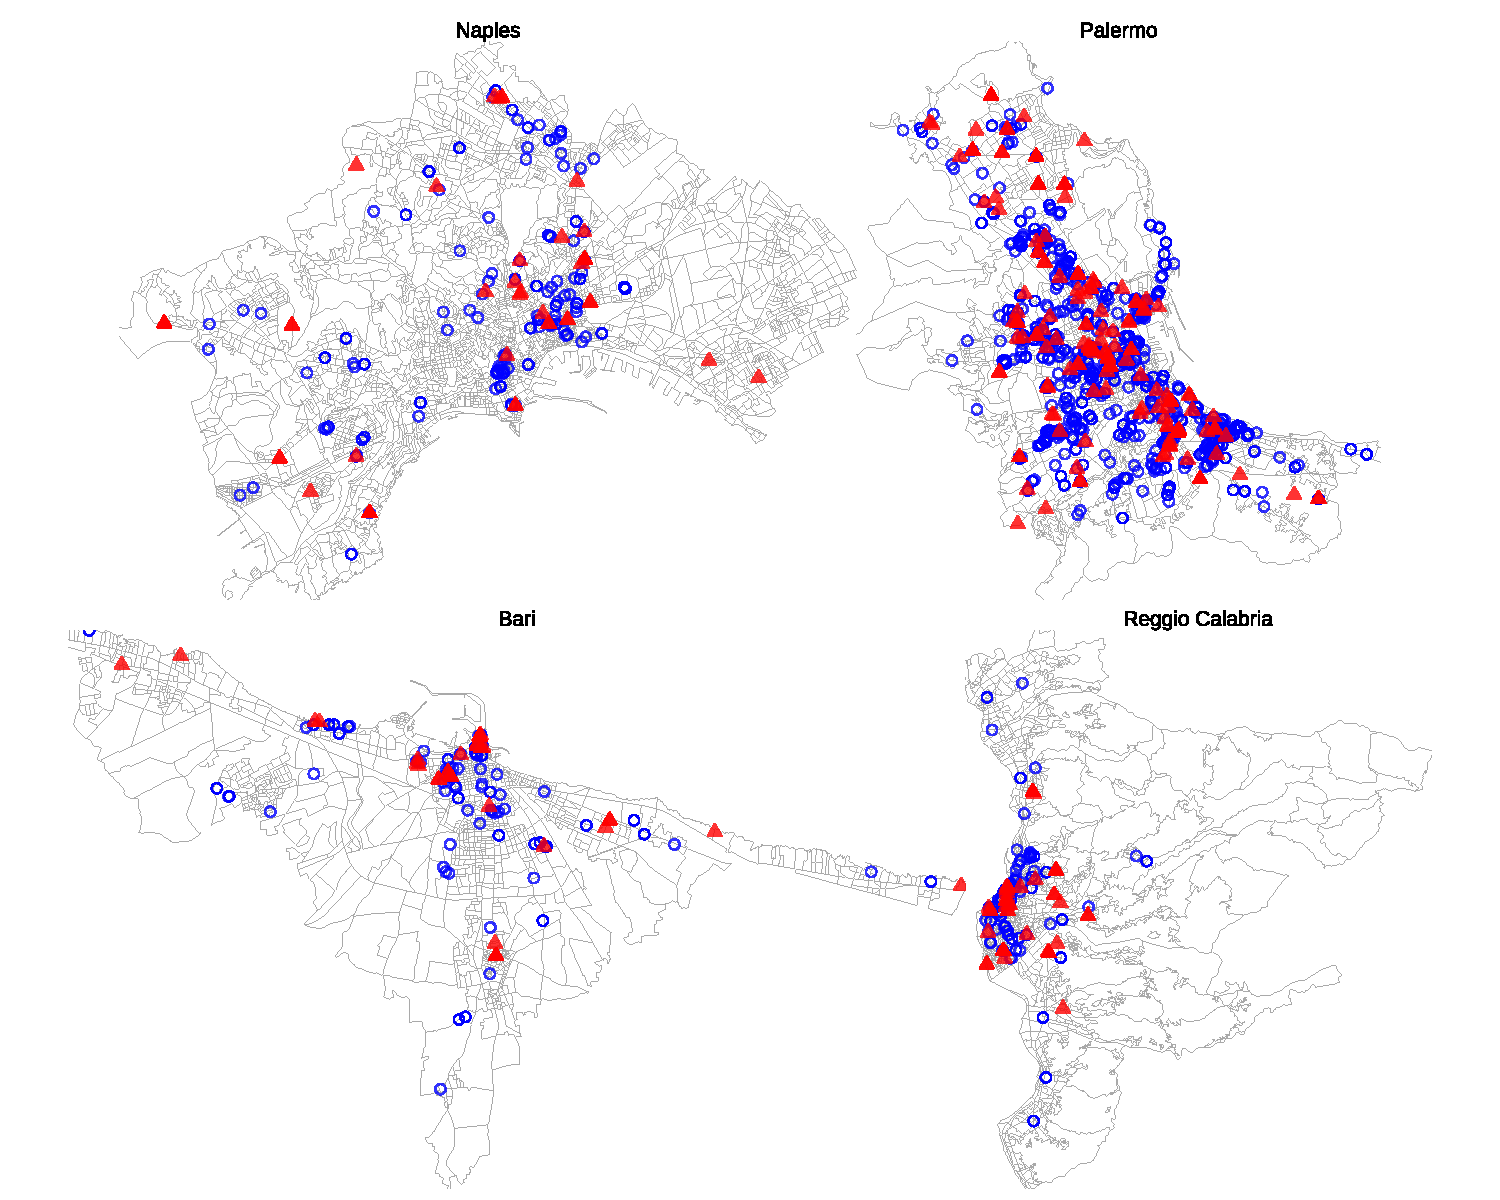
\includegraphics[scale=0.56]{pictures_1/assets1.pdf}
    \centering
    \end{center}
    \end{figure}
      \begin{figure}[H]
  \begin{center}
    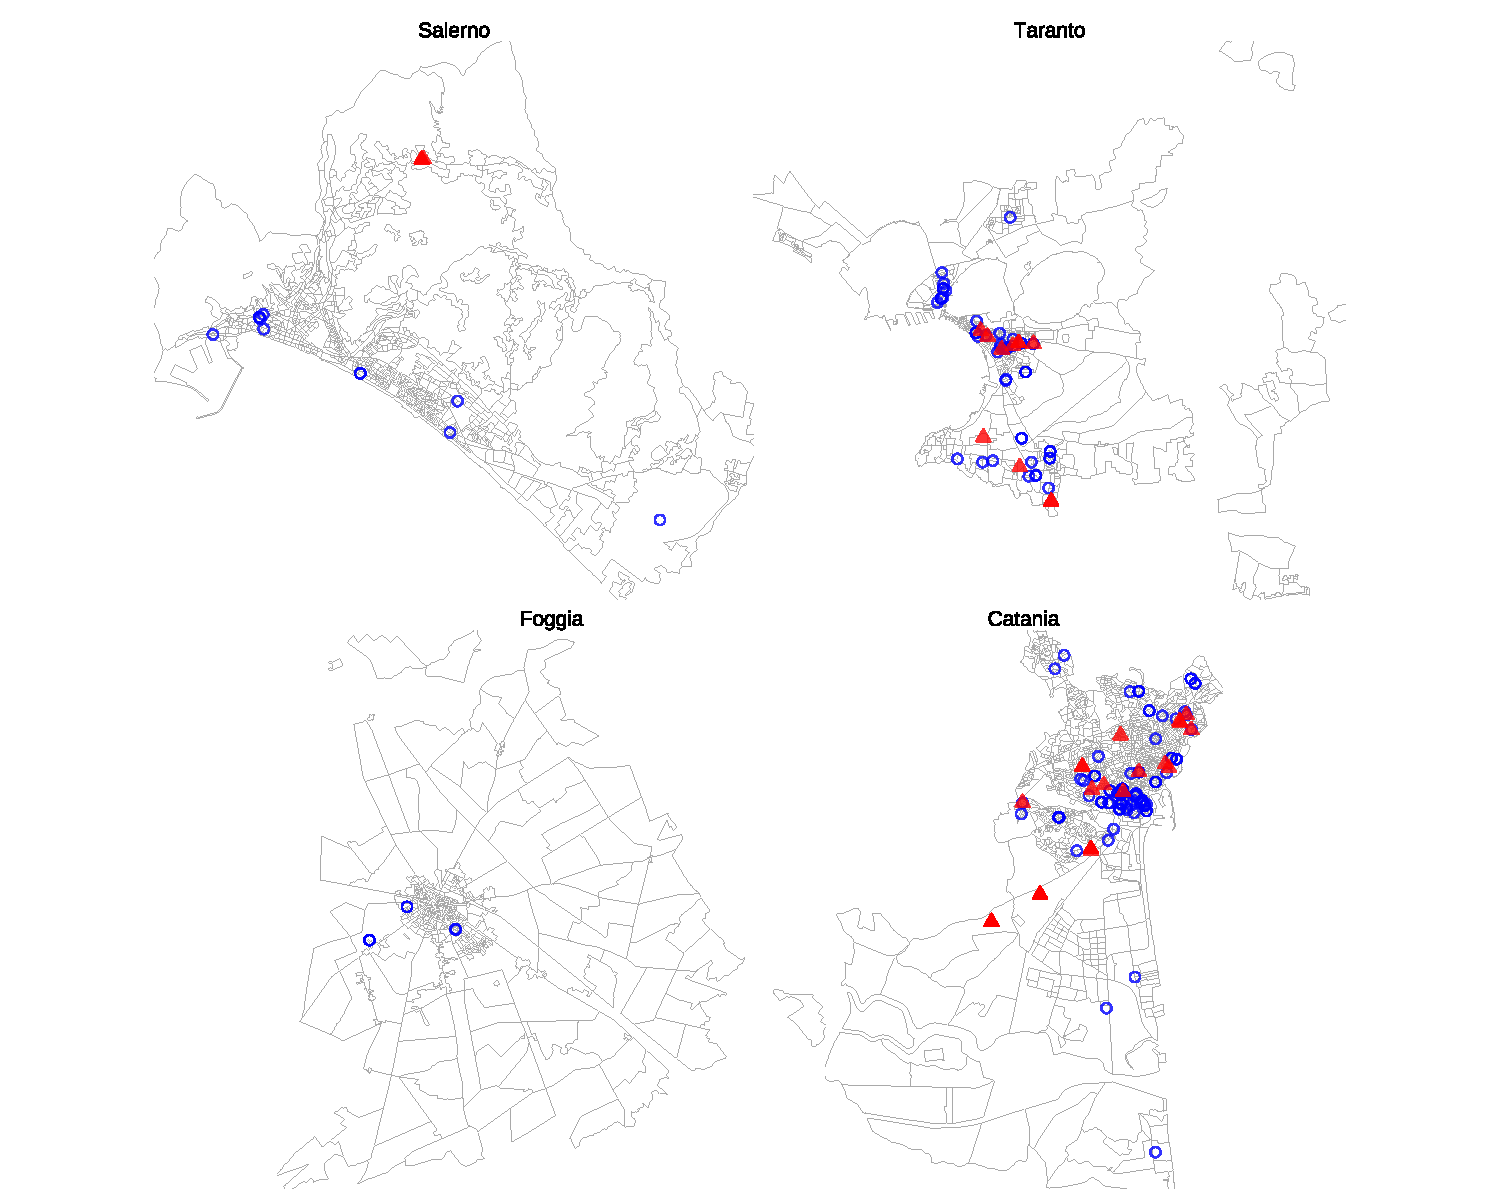
\includegraphics[scale=0.56]{pictures_1/assets2.pdf}
    \centering
    \end{center}
    \end{figure}
         \begin{figure}[H]
     \begin{center}
    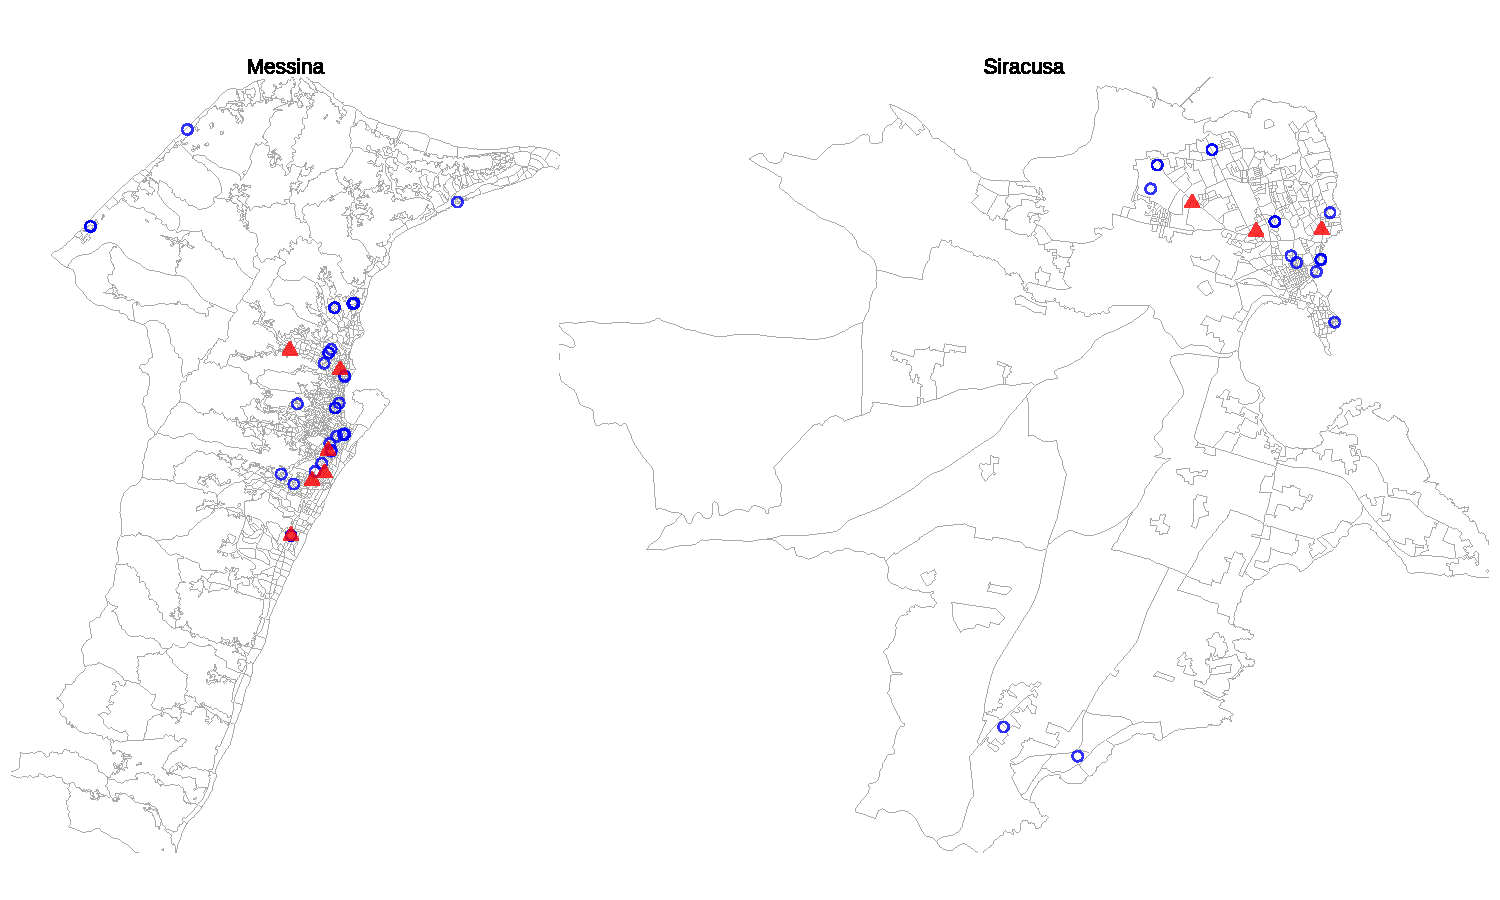
\includegraphics[scale=0.6]{pictures_1/assets3.pdf}
    \centering\caption{The distribution of Mafia real estate in the 10 metropolitan areas of the historical Mafia-ridden regions. Empty blue circles locate reallocated but not reused real estate, while red triangles indicate the real estate under reusing practices.}
    \label{fig:jmp_assets_map}
    \end{center}
    \end{figure}


\newpage

\renewcommand{\thefigure}{C.\arabic{figure}}
\renewcommand{\thetable}{C.\arabic{table}}
\setcounter{figure}{0}
\setcounter{table}{0}
\section{Endogeneity Concerns}
\label{sec:jmp_app_C}

\vspace{-0.3cm}
In this Appendix I investigate the determinants of the reuse of Mafia properties. \par
\vspace{0.2cm}

It is possible that an endogeneous treatment assignment violates the parallel trends assumption underlying the DiD identification strategy if the decision to reuse confiscated mafia properties is influenced by unobserved factors that also affect educational outcomes over time. While pure selection into treatment does not necessarily bias the results provided parallel trends hold, it is important to investigate the factors driving the reuse of Mafia properties to identify context-specific confounders. According to the CRR policy, local authorities are responsible for identifying local NGOs to manage reallocated Mafia properties and actively pursue their reuse for social activities. Although Table~\ref{tab:jmp_desc_stats} shows no significant differences in street-level characteristics between treated and untreated schools, treated schools might be systematically located in municipalities with stronger institutional capacity, higher civic engagement, or greater commitment to  put the policy into practice. Notably, these features can independently influence educational outcomes and create differential trends between treatment and control groups. \par
\medskip
To investigate this potential source of endogeneity, I estimate a linear probability model by regressing the probability of mafia property reuse on NGO presence in the year before reuse and several baseline municipality characteristics not controlled for in the main specification. Since reuse is measured in the year when the municipality and local NGO sign a management agreement, the level of NGO presence in the preceding period is crucial because municipalities must identify suitable partner organizations beforehand.
I collect several measures of municipal characteristics that could influence both reuse decisions and educational outcomes. First, I obtain information about whether municipalities were ever dissolved for mafia-related activities at baseline from \href{https://www.avvisopubblico.it/home/home/cosa-facciamo/informare/documenti-tematici/comuni-sciolti-per-mafia/}{Avviso Pubblico\footnote{Avviso Pubblico is an Italian national association created in 1996 to promote transparency in the public administration.}}. Second, I collect baseline municipal expenditure data from the \href{https://finanzalocale.interno.gov.it/banchedati.html}{Ministry of the Interior} for three relevant policy areas: youth policies, urban and territorial planning, and municipal police services. These expenditure categories capture municipal priorities and capacity in areas directly related to property reuse and community development. Finally, I create a transparency indicator equal to 1 for municipalities that failed to regularly publish information about available mafia properties for reuse on their websites before the first treatment occurrence. This measure follows the classification strategy implemented by  \citet{falcone_rimandati_2021, falcone_rimandati_2022} where municipalities where classified based on the level of trasparency shown online in sharing information about the presence of Mafia reallocated properties as inscribed by the law.  The model is specified as:\par

\begin{equation}
    P(Reuse=1)_{cm} = \beta_0 + \beta_1 lag_{NGO_{c}} + \beta_2 X'_{m} + \epsilon_{cm}
\end{equation}
\vspace{0.1cm}

where $P(Reuse=1)$ is the probability for a Mafia property to get reused in school catchment are $c$ in municipality $m$. $lag_{NGO}$ represents the number of NGOs active at the street-level one year before the reuse in school catchment area $c$, while $X'$ includes the aforementioned baseline municipalities features. \\
The results of the LPM are shown in Table~\ref{tab:jmp_lpm_predictors}. Column (3) shows that one additional NGO presence in the year prior to reuse significantly increases the probability of getting a reused Mafia property of 0.11\% relative to the mean. Although the mangitude of the effect is very small, this could indicate that areas with stronger organizational capacity are slightly more likely to receive reused properties. Several municipal characteristics also influence reuse decisions: first, municipalities with greater transparency in publishing information about reallocated Mafia properties seem to be more likely to pursue reuse; second, a doubling of territorial planning expenditure increases the probability of mafia property reuse by  7.79\%  relative to the mean, while doubling youth policy expenditure increases reuse probability by a relative 6.90\%. These substantial effects demonstrate that municipalities with stronger policy commitments and administrative capacity in areas directly relevant to community development and social programming are more likely to pursue reuse initiatives.  Notably, Mafia-related municipal dissolution experiences at the baseline do not predict reuse, indicating that treatment assignment is more on current institutional capacity rather than historical Mafia presence.\par


\begin{table}[H]
\caption{Robustness exercise including time trends and additional controls} % Table label
\label{tab:jmp_lpm_predictors}
\vspace{0.2cm}
\centering
\scalebox{0.85}{
      \begin{tabular}{p{9.28em}lll}
    \toprule
    \multicolumn{1}{l}{} & \multicolumn{1}{c}{(1)} & \multicolumn{1}{c}{(2)} & \multicolumn{1}{c}{(3)} \\
    \multicolumn{1}{r}{} & \multicolumn{3}{c}{P(Reuse = 1)} \\
    \midrule
    \multicolumn{1}{l}{} & \multicolumn{1}{c}{} & \multicolumn{1}{c}{} & \multicolumn{1}{c}{} \\
    \multicolumn{1}{l}{NGOs t-1} & \multicolumn{1}{c}{0.000235*} & \multicolumn{1}{c}{} & \multicolumn{1}{c}{0.000940***} \\
    \multicolumn{1}{l}{} & \multicolumn{1}{c}{(0.000133)} & \multicolumn{1}{c}{} & \multicolumn{1}{c}{(0.000213)} \\
    \multicolumn{1}{l}{Dissolution = 1} & \multicolumn{1}{c}{} & \multicolumn{1}{c}{0.0627} & \multicolumn{1}{c}{-0.0309} \\
    \multicolumn{1}{l}{} & \multicolumn{1}{c}{} & \multicolumn{1}{c}{(0.0941)} & \multicolumn{1}{c}{(0.108)} \\
    \multicolumn{1}{l}{Transparency = 1} & \multicolumn{1}{c}{} & \multicolumn{1}{c}{0.228***} & \multicolumn{1}{c}{0.232***} \\
    \multicolumn{1}{l}{} & \multicolumn{1}{c}{} & \multicolumn{1}{c}{(0.0642)} & \multicolumn{1}{c}{(0.0644)} \\
    \multicolumn{1}{l}{Exp youth policies} & \multicolumn{1}{c}{} & \multicolumn{1}{c}{0.0364} & \multicolumn{1}{c}{0.0594**} \\
    \multicolumn{1}{l}{} & \multicolumn{1}{c}{} & \multicolumn{1}{c}{(0.0239)} & \multicolumn{1}{c}{(0.0258)} \\
    \multicolumn{1}{l}{Exp education} & \multicolumn{1}{c}{} & \multicolumn{1}{c}{0.0225} & \multicolumn{1}{c}{0.000454} \\
    \multicolumn{1}{l}{} & \multicolumn{1}{c}{} & \multicolumn{1}{c}{(0.0139)} & \multicolumn{1}{c}{(0.0152)} \\
    \multicolumn{1}{l}{Exp urban planning} & \multicolumn{1}{c}{} & \multicolumn{1}{c}{0.0413***} & \multicolumn{1}{c}{0.0671***} \\
    \multicolumn{1}{l}{} & \multicolumn{1}{c}{} & \multicolumn{1}{c}{(0.0121)} & \multicolumn{1}{c}{(0.0151)} \\
    \multicolumn{1}{l}{Exp municipal police} & \multicolumn{1}{c}{} & \multicolumn{1}{c}{-0.0204} & \multicolumn{1}{c}{-0.000231} \\
    \multicolumn{1}{l}{} & \multicolumn{1}{c}{} & \multicolumn{1}{c}{(0.0148)} & \multicolumn{1}{c}{(0.0157)} \\
    \multicolumn{1}{l}{} & \multicolumn{1}{c}{} & \multicolumn{1}{c}{} & \multicolumn{1}{c}{} \\
    \multicolumn{1}{l}{clustered SE} & \multicolumn{1}{c}{yes} & \multicolumn{1}{c}{yes} & \multicolumn{1}{c}{yes} \\
    \multicolumn{1}{l}{Observations} & \multicolumn{1}{c}{1,746} & \multicolumn{1}{c}{2,096} & \multicolumn{1}{c}{1,746} \\
    \multicolumn{1}{l}{Mean dep. var.} & \multicolumn{1}{c}{0.861} & \multicolumn{1}{c}{0.857} & \multicolumn{1}{c}{0.861} \\
    \midrule
    \multicolumn{4}{p{24.28em}}{Notes: LPM model. The outcome variable is equal to 1 whenever there is at least one Mafia property within the school catchment area. Standard errors are clustered at the school level.} \\
    \end{tabular}%
    }
    \end{table}

To address this endogeneity concerns, I re-estimate the main DiD specification including a control for the lagged presence of NGOs and municipality-specific time trends. This way, I test whether the estimated effect of the reuse of Mafia properties reuse dropout rates are robust after accounting for systematic differences in NGOs and municipal characteristics. Table~\ref{tab:jmp_reuse_predictors} shows the baseline and the re-estimated results. This exercise demonstrates that the negative effect of reuse activities on dropout rates persists even after controlling for the systematic factors that drive treatment assignment. Comparing the baseline specifications presented in Columns (1) and (2) with the specification accounting for both NGOs and municipalities characteristics in Column (4), the estimated treatment effect remains statistically significant and economically meaningful, declining only by  5.3\% relative to the mean. This represents a reduction to the mean from 36.2\% to 31.4\%, so there is still a substantial 31\% decrease in dropout rates. Column (5) replaces municipality-specific time trends with municipality×year fixed effects, the most saturated specification. The point estimate remains stable at -0.0159 but falls just short of conventional significance levels (t = 1.56, p = 0.120). The identification employed in this specification relies exclusively on within-municipality, across-school variation in treatment status in a given year. However, the share of treated schools within municipality-year cells is very close to 0 or 1 in for roughtly half of the sample, presenting no within-year variation. This indicates that most treatment variation is between rather than within municipalities, and that municipality X year FEs absorb the bulk of the identifying variation, mechanically reducing statistical power. The persistence of a large negative coefficient across all specifications provides clear evidence that the relationship between reuse activities and improved educational outcomes is robust to concerns about systematic treatment assignment based on local organisational capacity.


\begin{table}[H]
\caption{Estimating reuse predictors}
\label{tab:jmp_reuse_predictors}
\vspace{0.2cm}
\centering
\scalebox{0.85}{
    \begin{tabular}{p{10.555em}lllll}
    \toprule
    \multicolumn{1}{l}{} & \multicolumn{1}{c}{(1)} & \multicolumn{1}{c}{(2)} & \multicolumn{1}{c}{(3)} & \multicolumn{1}{c}{(4)} & \multicolumn{1}{c}{(5)} \\
    \multicolumn{1}{r}{} & \multicolumn{5}{c}{\textbf{Dropout rate G11-G13}} \\
    \midrule
    \multicolumn{1}{l}{} & \multicolumn{1}{c}{} & \multicolumn{1}{c}{} & \multicolumn{1}{c}{} & \multicolumn{1}{c}{} & \multicolumn{1}{c}{} \\
    \multicolumn{1}{l}{Reuse = 1} & \multicolumn{1}{c}{-0.0192**} & \multicolumn{1}{c}{-0.0196**} & \multicolumn{1}{c}{-0.0168*} & \multicolumn{1}{c}{-0.0166*} & \multicolumn{1}{c}{-0.0159} \\
    \multicolumn{1}{l}{} & \multicolumn{1}{c}{(0.00934)} & \multicolumn{1}{c}{(0.00943)} & \multicolumn{1}{c}{(0.00981)} & \multicolumn{1}{c}{(0.00979)} & \multicolumn{1}{c}{(0.01017)} \\
    \multicolumn{1}{l}{} & \multicolumn{1}{c}{} & \multicolumn{1}{c}{} & \multicolumn{1}{c}{} & \multicolumn{1}{c}{} & \multicolumn{1}{c}{} \\
    \multicolumn{1}{l}{Clustered SE} & \multicolumn{1}{c}{yes} & \multicolumn{1}{c}{yes} & \multicolumn{1}{c}{yes} & \multicolumn{1}{c}{yes} & \multicolumn{1}{c}{yes} \\
    \multicolumn{1}{l}{Student migration} & \multicolumn{1}{c}{no} & \multicolumn{1}{c}{yes} & \multicolumn{1}{c}{no} & \multicolumn{1}{c}{yes} & \multicolumn{1}{c}{yes} \\
    \multicolumn{1}{l}{Grade retention} & \multicolumn{1}{c}{no} & \multicolumn{1}{c}{yes} & \multicolumn{1}{c}{no} & \multicolumn{1}{c}{yes} & \multicolumn{1}{c}{yes} \\
    \multicolumn{1}{l}{NGO lags} & \multicolumn{1}{c}{no} & \multicolumn{1}{c}{no} & \multicolumn{1}{c}{yes} & \multicolumn{1}{c}{yes} & \multicolumn{1}{c}{yes} \\
    \multicolumn{1}{l}{Municipality time trends} & \multicolumn{1}{c}{no} & \multicolumn{1}{c}{no} & \multicolumn{1}{c}{yes} & \multicolumn{1}{c}{yes} & \multicolumn{1}{c}{no} \\
    \multicolumn{1}{l}{Municipality $\times$ year FE} & \multicolumn{1}{c}{no} & \multicolumn{1}{c}{no} & \multicolumn{1}{c}{no} & \multicolumn{1}{c}{no} & \multicolumn{1}{c}{yes} \\
    \multicolumn{1}{l}{Observations} & \multicolumn{1}{c}{1,296} & \multicolumn{1}{c}{1,272} & \multicolumn{1}{c}{1,284} & \multicolumn{1}{c}{1,262} & \multicolumn{1}{c}{1,262} \\
    \multicolumn{1}{l}{Number of schools} & \multicolumn{1}{c}{235} & \multicolumn{1}{c}{234} & \multicolumn{1}{c}{234} & \multicolumn{1}{c}{233} & \multicolumn{1}{c}{233} \\
    \multicolumn{1}{l}{Mean dep. var.} & \multicolumn{1}{c}{0.0537} & \multicolumn{1}{c}{0.0531} & \multicolumn{1}{c}{0.0536} & \multicolumn{1}{c}{0.0529} & \multicolumn{1}{c}{0.0529} \\
    \midrule
    \multicolumn{6}{p{35em}}{Notes: TWFE model. The treatment variable is equal to 1 whenever there is at least one Mafia property within the school catchment area. Standard errors are clustered at the school level.} \\
    \end{tabular}%
    }
\end{table}

\newpage
\renewcommand{\thefigure}{D.\arabic{figure}}
\renewcommand{\thetable}{D.\arabic{table}}
\setcounter{figure}{0}
\setcounter{table}{0}
\FloatBarrier
\section{Construction of Additional Variables}
\label{sec:jmp_app_D}
\vspace{-0.3cm}
This appendix provides additional information on the data and variables used in this paper. \par
\vspace{0.2cm}


    \medskip
\textbf{\emph{Schools' catchment areas.}} To test whether the treatment allocation and results are sensitive to changes in the construction of school catchment areas, I build an alternative version where I weight the Euclidean distance used to assign census blocks to schools based on schools' capacity. I proceed in three steps: first, I aggregate census blocks to their closest school based on simple Euclidean distance. Second, I multiply the distance by the average enrollment rate of each school and divide the result by each school's enrollment rate at the baseline as follows:

\begin{equation*}
d_{ic}^* = d_{ic} \times \frac{\bar{E}}{E_i}
\end{equation*}

This way, schools with higher capacity, which show an above-average enrollment, will display larger catchment areas, accounting for supply-side factors in the allocation of census blocks. Third, I repeat this process for each of the 14 schools' specialisations to consistently align with a location-allocation approach. Only 17 of the sample schools change their treatment status under these new assumptions, relaxing the concern about artificial treatment allocation.
Figure~\ref{fig:catchment_comparison} compares schools' catchment areas obtained using Euclidean and weighted-Euclidean distances for language academic high schools in Naples.

As expected, capacity-weighted catchment areas show slightly different boundaries. I employ this alternative specification solely for robustness testing in Section~\ref{sec:jmp_selection_bias}, where I examine treatment effects only in areas with unchanged boundaries to assess whether the main results are driven by schools with ambiguous treatment allocation across the two construction methods. \par

  \begin{figure}[H]
  \begin{center}
    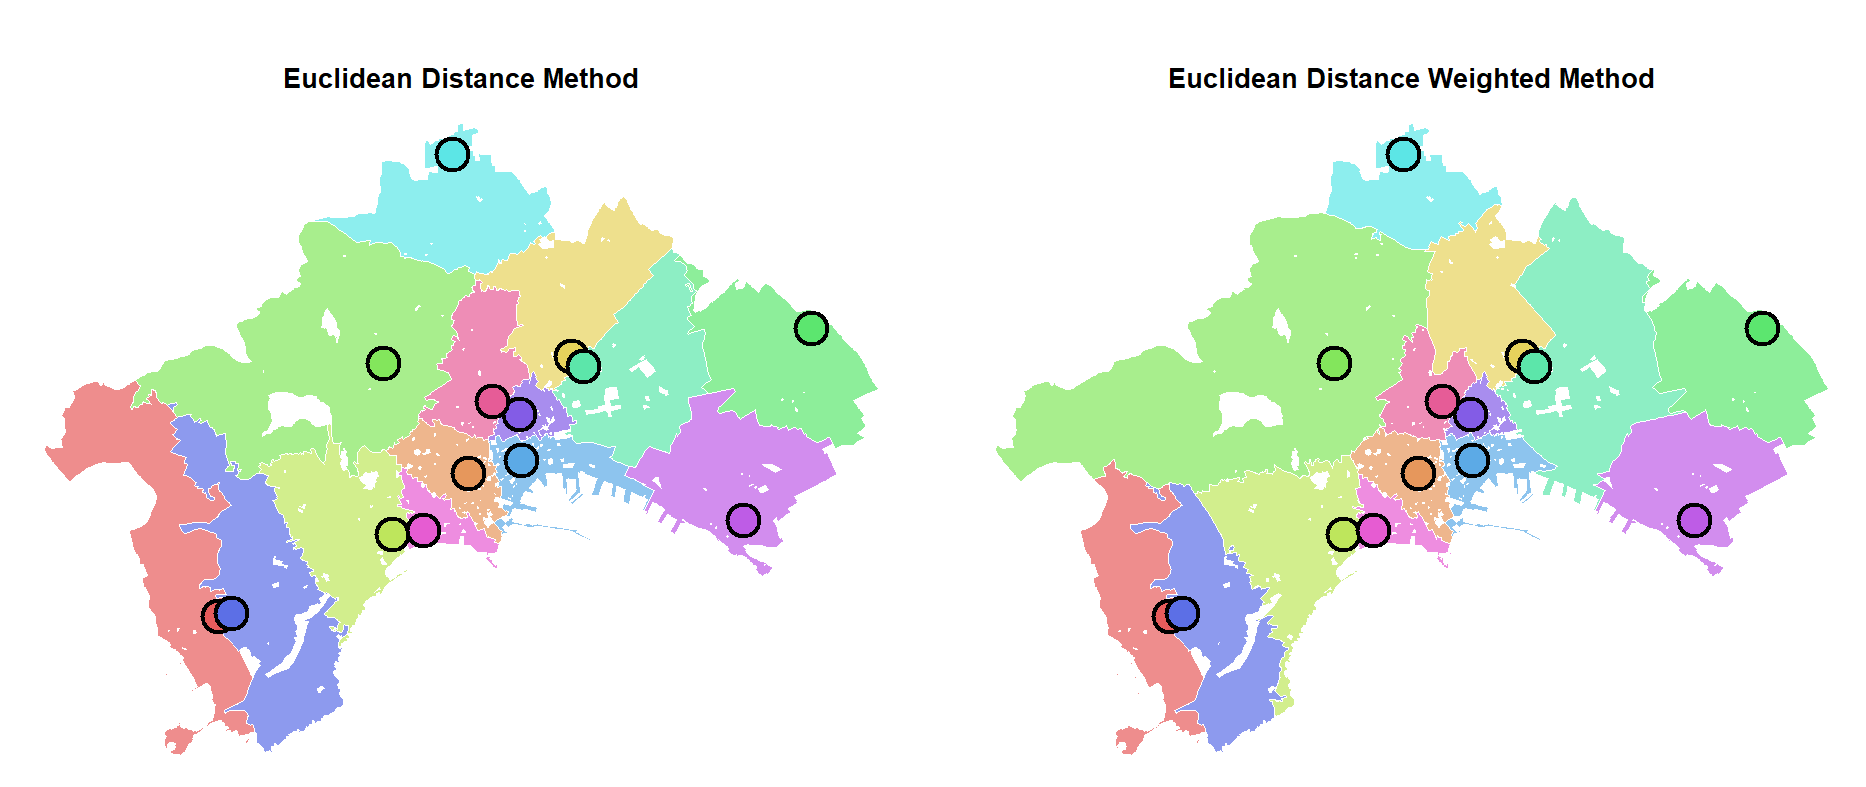
\includegraphics[scale=0.42]{pictures_1/capacity_dist_1025.png}
    \centering
    \label{fig:catchment_comparison}
    \caption{Schools' catchment areas measured with Euclidean distance (left) and capacity-weighted distance (right)}
    \end{center}
    \end{figure}


\textbf{\emph{Students' migration.}} I report below the measure I compute to control for school-specific students' migration patterns, as explained in Section~\ref{sec:jmp_other_data}.  I rely on the assumption that students who disappear from enrollment registries before turning 16 are more likely to be transferring to other schools rather than genuinely dropping out, given that education is compulsory until the age of 16. I build this measure following the same construction methodology as the main outcome variable, but capturing the share of students who do not complete grades 9 and 10 as their first and second years of high school.
The measure is reported in Equation 6. Starting from the cohort of students who completed grades from 9 to 11 in year $t-1$, I subtract those who progressed to complete grade 12 in year $t$, and those who completed grades 10 and 11 in year $t$, expressing this as a share of the initial cohort who completed grades from 9 to 11 in year $t-1$. \par
\vspace{0.3cm}
\begin{equation}
Dropout_{G9-11{_t}} = \frac{Completed_{G9-11_{t-1}}-Completed_{G12_{t}}-Completed_{G10-11_t}}{{Completed_{G9-11_{t-1}}}}
\end{equation}
\vspace{0.3cm}

 \textbf{\emph{Grade retention rate.}}  It is possible that students repeating years due to inadequate academic performance will confound my measure of dropout by appearing enrolled in the same grade for both time $t-1$ and time $t$. To address this, I construct a proxy for grade retention rates for students enrolled on grades 11, 12, and 13. Figure~\ref{fig:jmp_age_grade} in Section~\ref{sec:jmp_schools_data} shows that students following the standard educational timeline are expected to be 16 or 17 years old in grade 11, and 17 or 18 years old in grade 12.

I calculate the share of students repeating grade 11 as the number of students aged 18 or older as a share of all students completing grade 11 in time $t$. Similarly, the share of students repeating grade 12 is calculated as the number of students aged 19 or older as a share of all students completing grade 12 in time $t$. Equations 7 and 8 show the respective grade retention rates. Due to data limitations, I cannot compute the retention rate for grade 13, as I cannot observe whether students are older than 19 in grade 13. However, since the average retention rate declines from 1.2\% in grade 11 to zero in grade 12, the grade 13 retention rate would likely be negligible. 
 
\vspace{0.3cm}
\begin{equation}
Retention_{G11{_t}} = \frac{aged18_{G11{_t}}}{{Completed_{G11_{t}}}}
\end{equation}
\vspace{0.3cm}
\begin{equation}
Retention_{G12{_t}} = \frac{aged19+_{G12{_t}}}{{Completed_{G12_{t}}}}
\end{equation}
\vspace{0.3cm}


  \textbf{\emph{Schools' quality index.}}  I construct a composite baseline indicator of school quality, drawing on two dimensions evaluated through a structured assessment framework used by the Italian schools, namely the annual Self-Evaluation Report (RAV). The first dimension, focusing on the school-level learning outcomes, encompasses four criteria: school grades, standardised test scores, civic competences, and long-term outcomes. The second dimension, which focuses on learning process, covers seven criteria related to the organisational and pedagogical functioning of the school: module planning, learning environment, inclusion and diversity, student guidance, school organisation, human resources development, and integration with the local community. For each dimension, I construct a sub-index by taking the row mean of the standardised scores assigned to each criterion of learning outcomes performance and learning process performance, respectively. The overall school performance indicator is then computed as the simple average of these two sub-indices, giving equal weight to outcomes and processes. This produces a composite score at the school level that captures both what students achieve and how the school operates to support that achievement, and serves as the baseline measure of school quality in the analysis.
  
\begin{table}[H]
\centering
\caption{RAV School Quality Indicators}
\scalebox{0.75}{
    \begin{tabular}{rr|r|rr}
    \toprule
    \multicolumn{2}{c|}{\textbf{Learning Outcomes}} &       & \multicolumn{2}{c}{\textbf{Learning Process}} \\
    \midrule
    \multicolumn{1}{c}{\textbf{ID criteria}} & \multicolumn{1}{l|}{\textbf{Description}} &       & \multicolumn{1}{c}{\textbf{ID criteria}} & \multicolumn{1}{l}{\textbf{Description}} \\
    \multicolumn{1}{c}{21} & \multicolumn{1}{l|}{School grades} &       & \multicolumn{1}{c}{31} & \multicolumn{1}{l}{Modules planning } \\
    \multicolumn{1}{c}{22} & \multicolumn{1}{l|}{Standardised test scores} &       & \multicolumn{1}{c}{32} & \multicolumn{1}{l}{Learning environment} \\
    \multicolumn{1}{c}{23} & \multicolumn{1}{l|}{Civic competences} &       & \multicolumn{1}{c}{33} & \multicolumn{1}{l}{Inclusion and diversity} \\
    \multicolumn{1}{c}{24} & \multicolumn{1}{l|}{Long-term outcomes} &       & \multicolumn{1}{c}{34} & \multicolumn{1}{l}{Student giudance} \\
          &       &       & \multicolumn{1}{c}{35} & \multicolumn{1}{l}{School organisation} \\
    \multicolumn{2}{c|}{} &       & \multicolumn{1}{c}{36} & \multicolumn{1}{l}{HR development} \\
          &       &       & \multicolumn{1}{c}{37} & \multicolumn{1}{l}{Integration with the local community} \\
          &       &       &       &  \\
    \bottomrule
    \end{tabular}%
    }
    \end{table}


 \textbf{\emph{Heterogeneous effects of repurposing.}} To assess whether the estimated effects are driven by a specific type of activity offered in the repurposed properties, I decompose the treatment effect by activity category (education, employment, welfare, culture). Because these categories are not mutually exclusive — a single school catchment area may contain several repurposed properties offering different types of activity — I estimate a separate regression for each category rather than including all categories jointly. Within each regression, I split treated areas into two groups according to whether they offer the activity of interest, and compare both against the same set of never- and not-yet-treated control areas. Formally, for a given activity category I estimate
 	\begin{equation}
 	DropoutG11\text{-}G13_{cnmt} = \beta_1 (Category =1)_{ct} + \beta_2 (Category = 0)_{ct} + \beta_3 X'{ct} + \delta{c} + \eta_{t} + \epsilon_{cnmt}
 \end{equation}
 
 where $(Category =1)_{ct}$ equals 1 when the school catchment area contains at least one repurposed property offering activities of the relevant type, and $(Category = 0)_{ct}$ equals 1 when area $c$ is treated but none of its repurposed properties offer that type of activity. Control areas take the value zero for both indicators and serve as the omitted reference group. The vector $X'_{ct}$ contains the same controls as in the baseline specification, and $\delta_c$ and $\eta_t$ denote catchment-area and time fixed effects, respectively. Standard errors are clustered at the school level. The coefficient $\beta_1$ captures the dropout effect in treated areas that provide the activity in question, while $\beta_2$ captures the effect in treated areas that do not. Comparing the two isolates the marginal contribution of each activity type: if a category were the main driver of the overall effect, its $\beta_1$ should be substantially larger in magnitude, and more precisely estimated, than the corresponding $\beta_2$. The estimates are reported in Figure~\ref{fig:jmp_cats_repurpose}. \\
\clearpage
% Here, you create your reference list. These commands automatically create a list of references that contains exactly those entries that have cited in the text using the citation commands described above.
% this refers to the file econ.bst, which defines the style in which the references are set. The file must be placed in the same folder as the current .tex file


\clearpage
% Here, you create your reference list. These commands automatically create a list of references that contains exactly those entries that have cited in the text using the citation commands described above.
% this refers to the file econ.bst, which defines the style in which the references are set. The file must be placed in the same folder as the current .tex file


\bibliographystyle{econ} 
\bibliography{referenceszotero} % this refers to the file bibtemplate.bib, which contains all necessary bibliographical information on the referenced work


\end{document}